\documentclass{article}
\usepackage{amsmath,amssymb}
\usepackage{bm}
\usepackage[numbers,sort&compress]{natbib}
\usepackage{graphicx}
\usepackage{color}
\usepackage{tabularx}
\usepackage{leftidx}

\newcommand{\beq}{\begin{equation}}
\newcommand{\feq}{\end{equation}}
\newcommand{\beqstar}{\begin{equation*}}
\newcommand{\feqstar}{\end{equation*}}                                     
\newcommand{\beqal}{\begin{equation}\begin{aligned}}
\newcommand{\feqal}{\end{aligned}\end{equation}}
\newcommand{\beqalstar}{\begin{equation*}\begin{aligned}}
\newcommand{\feqalstar}{\end{aligned}\end{equation*}}
\newcommand{\kl}{k_L}
\newcommand{\vol}{k_L\,a}
\newcommand{\lbubble}{L_{\mathrm{bubble}}}
\newcommand{\lunit}{L_{\mathrm{unit}}}
\newcommand{\lslug}{L_{\mathrm{slug}}}
\newcommand{\lfilm}{L_{\mathrm{film}}}
\newcommand{\ububble}{U_{\mathrm{bubble}}}
\newcommand{\uliq}{U_{\mathrm{liq}}}
\newcommand{\ugas}{U_{\mathrm{gas}}}
\newcommand{\uoutlet}{U_{\mathrm{outlet}}}
\newcommand{\cbubble}{C_{\mathrm{bubble}}}
\newcommand{\cinlet}{C_{\mathrm{inlet}}}
\newcommand{\coutlet}{C_{\mathrm{outlet}}}
\newcommand{\coverall}{C_{\mathrm{overall}}}
\newcommand{\cstar}{C^{*}}
\newcommand{\cmedium}{C_{\mathrm{medium}}}
\newcommand{\volnondim}{\vol \frac{\lunit}{\ububble+\ugas}}
\newcommand{\omegaplus}{\omega_{+}}
\newcommand{\omegaminus}{\omega_{-}}
\newcommand{\holdup}{\varepsilon_{\mathrm{gas}}}

\title{Lattice Boltzmann study of mass transfer for Bretherton/Taylor bubble train flow}

\begin{document}
\maketitle
\begin{abstract}
This work presents a thorough procedure of how to determine the volumetric mass transfer
coefficient
in the context of lattice Boltzmann simulations for the Bretherton/Taylor bubble train flow. In this work we address the situation when the hydrodynamic pattern changes from having a vortex in slug ($Ca<0.7$) to not having it ($Ca>0.7$) \cite{giavedoni-numerical}. For the latter case the bubble shape is not symmetric and cannot be approximated through flat surfaces and circumferences as it is done in literature \cite{vanbaten-circular,kreutzer-overview}. Moreover, with a vortex in the slug the tracer is well mixed. Thus, it is common to  use periodic boundary conditions  and inlet/outlet averaged concentration as the characteristic concentration, Eq. \ref{eq:main:definition}.  The later is not valid for flows where tracer is not well mixed. This work through examination of different boundary conditions and different characteristic concentration definitions establishes the procedure to determine the volumetric mass transfer coefficient for flows with the capillary number $0.1<Ca<1.0$. With simulations of a few unit cells the connection between time (used in simulations) and space (used in experiments) domains was established. The following boundary conditions were examined: periodic boundary conditions, open boundaries, and a few unit cells open boundary
simulations. It was shown that the time dependent average concentration to be a characteristic
concentration produce robust results, though a bit overpredicted. The inlet/outlet flux averaged
concentration \cite{vanbaten-circular} to be a characteristic concentration produce unreliable results in the range of capillary numbers specified. In comparison with works \cite{vanbaten-circular,kreutzer-overview} where only one unit cell was simulated, a few
unit cells open boundaries conditions resemble physical situation most closely and are harder to conduct
but provide the volumetric mass transfer coefficient based only on the spatial information for the
capillary number $Ca>0.7$. 
%As well, a few unit cells simulations can provide more information about
%mixing in the liquid slug in comparison with the periodic boundary conditions. 
We show
that all presented in literature strategies are extreme limits of one equation,
Eq. \ref{main:main:main}. Finally, simulation results for different Peclet numbers
are compared with analytical predictions presented by \citet{vanbaten-circular} and shows a good
agreement. The work is of use to people performing mass transfer numerical simulations for bubble
train flow in microchannels and/or within the
lattice Boltzmann context.
\end{abstract}

\section{Introduction}
\label{intro}
The monolith reactors during last years are getting more attention as a promising alternative to slurry
reactors and trickle bed reactors \cite{kreutzer-overview,bercic-mass}. Reactors usually operate in Bretherton-Taylor regime \cite{bretherton,taylor} which describes a flow through
a liquid medium of equally sized, long bubbles, see
Fig. \ref{fig:benchmark:hydro}. This flow regime
is characterized by surface tension dominance over inertia and viscous effects, and by
comparatively small gas flow velocities \cite{yue-mass}. Due to surface tension dominance bubble train flow exhibit advantageous properties which can not be achieved
in macroscopic counterparts: liquid thin films \cite{bretherton} between bubbles and walls remarkably enhance mass
transfer from a gas and walls to liquid; the plug flow regime occurring in monolith reactors allows to perform chemical reactions in slugs only \cite{kreutzer-overview}. Moreover, the low slip velocity between gas and liquid is utilized in the experiments to measure liquid velocity \cite{taylor}:  bubbles travelling with approximately the same velocity as liquid can be captured with a camera. Overall, nowadays one can find a large number of applications
of the Bretherton-Taylor bubble train flow: continuous flow analyzers to measure liquid velocity, lung openings, chemical reactions
as hydrogenation of nitroaromatics, 2-ethyl-hexenal, Fischer-Tropsch synthesis, etc. Extensive reviews of \citet{kreutzer-overview,
gupta-review,yue-mass} cover a significant number of applications. 

This work is focused on the gas to liquid mass transfer 
study for the Bretherton/Taylor flow. The good understanding of mass transfer and how it depends on the
parameters as the capillary number, the Reynolds number, slug and bubble lengths allows to properly
manufacture a microchannel with necessary properties to ensure that chemical
reactions are performed in the best manner. The mass transfer coefficient characterizing mass transfer is defined as the flux from the surface divided on the concentration difference between the concentration imposed on the body and the characteristic concentration in the domain. The characteristic concentration in the domain depends largely on underlying hydrodynamics fields.  For example, experimental studies \cite{yue-mass,bercic-mass} show a complex dependency of the mass transfer coefficient on flow parameters: bubble and slug lengths, bubble velocity, which are in turn depend on the capillary number $Ca$ and the Reynolds number $Re$. 
\citet{yue-mass} established an experimental correlation for the volumetric mass transfer coefficient for a bubble train as
a function of the diffusion coefficient, slug and bubble lengths, and bubble velocity: 
\begin{equation}
\vol =\frac{2}{d_h} \Bigl(\frac{D
\ububble}{\lbubble+\lslug}\Bigr)^{0.5}
\Bigl(\frac{\lbubble}{\lbubble+\lslug}\Bigr)^{0.3},
\end{equation}
where $\vol$ is the volumetric mass transfer coefficient, $d_h$ is the hydrodynamic capillary
diameter, $\lbubble$ is the bubble length, $\lslug$ is the slug distance (between bubbles),
$\ububble$ is the bubble velocity, $D$ is the diffusion coefficient. 
%This correlation is within $10\%$ accuracy for experimental
%results for the microchannels with rectangular/square crosssections for the following range of
%parameters: bubble velocity $0.4\,\mathrm{m/s}<\ububble<2\,\mathrm{m/s}$, bubble length
%$1.4<\frac{\lbubble}{d_h}<6.3$, slug length $1<\frac{\lslug}{d_h}<3.2$,
%hydrodynamic diameter $d_h = 400 \mathrm{\mu m}$.

Thus, the understanding of mass transfer for the bubble train flow is not possible without deep understanding of hydrodynamic patterns. There are a number of studies available for the hydrodynamic study of the bubble train flow: experimental \cite{kreutzer-pressure-drop,cerro-space,cerro-bubble-train} and numerical \cite{wang-non-circular,kuzmin-binary3d,giavedoni-numerical,heil-threedim}. For the flow of long bubbles between parallel plates as the study case it is indicated that  there exists a vortex in the liquid slug for $Ca<0.7$ , see Fig. \ref{fig:streamlines:tweaked:velocity}. However, for $Ca>0.7$ the vortex in the liquid slug does not exist. As well the bubble shape for low capillary numbers ($Ca<0.1$ \cite{cerro-bubble-train}) is symmetric. Thus, in the case of flow between plates the bubble shape can be represented as two hemicircles and two planar interfaces. This is heavily utilized for mass transfer analytical estimations.

As mentioned before the mass transfer coefficient is defined as the mass flux from certain area, Eq. \ref{eq:main:definition}. Thus, analytical estimations \cite{kreutzer-overview,irandoust} are  based on decomposition of the bubble shape. The mass transfer coefficient is calculated through two separate contributions from two films and two hemicircles. For both contributions the Higbie penetration theory \cite{higbie} is utilized, which states that the mass transfer coefficient  for simple geometry flow depends on the average time of liquid packet interaction with a geometrical feature. It can be calculated as $\sqrt{\frac{\pi D}{t_{\mathrm{char}}}}$, where $t_{\mathrm{char}}$ is the interaction characteristic time, $D$ is the diffusion coefficient. As the example for the Higbie penetration theory, the mass  transfer coefficient for the flow of bubbles between parallel plates  is calculated as (similarly to work of \citet{vanbaten-circular}):
\beq
k_L=2 \sqrt{\frac{\pi D}{t_{\mathrm{film}}}}+2 \sqrt{\frac{\pi D}{t_{\mathrm{circle}}}},
\feq
where $t_{\mathrm{film}}=\frac{\lfilm}{\ububble}$ states for the interaction time of liquid traveling through planar part of the bubble, $t_{\mathrm{circle}}=\frac{\pi R_{\mathrm{circle}}}{\ububble}$ is the time which liquid in the slug travels the distance of half circumference. 

Despite the simplicity, analytical expressions work well for flows with low capillary numbers $Ca<0.1$ \cite{bercic-mass} where the bubble shape is symmetrical and can be nicely approximated. Moreover, because of the hydrodynamic pattern in the slug, i.e. there is a vortex in slug, one can estimate the time for fluid batch to travel whole circumference.   However, with the change of the capillary number the situation drastically changes. The symmetrical bubble shape changes and resembles a bullet \cite{kuzmin-binary2d}. With the change of the shape and for flows with $Ca>0.7$ there is no vortex in the liquid slug. In this case the Higbie theory fails to estimate contribution from bubble caps. Thus, the need of numerical simulations where all hydrodynamics fields and complicated bubble shapes are taken in the account is obvious. 

However, available numerical studies of mass transfer \cite{kreutzer-overview,vanbaten-circular} are lacking the simulation of  bubble shapes. The usual simulation of the mass transfer  is performed as follows: 
\begin{description}
\item[I] The bubble shape is calculated either through analytical correlations \cite{bretherton} or experimental correlations \cite{cerro-bubble-train} without directly resolving bubbles shapes through multiphase simulations. 
\item[II] Hydrodynamics fields are then obtained by performing simulations of one-component flow around the droplet by imposing the bubble velocity on the walls. Thus, the simulations are performed in the reference frame moving with the bubble. The stress free condition is imposed at the bubble surface. 
\item[III]  The mass transfer simulations are  performed in the reference frame moving with the bubble. The saturation concentration is imposed at the bubble surface. Only one unit cell with one bubble in it is used for simulations. Periodic boundary conditions are utilized to determine the volumetric mass transfer coefficient, which is calculated through the following equation \cite{vanbaten-circular}:
\begin{equation}
\label{main:simulation:equation}
\vol=\frac{\mathrm{\overline{Flux}}}{\cbubble-\langle\coutlet\rangle} \frac{\mathrm{bubble\ surface\ area}}{\mathrm{unit\
cell\ volume}},
\end{equation}
where $\langle\coutlet(t)\rangle=\int{C \uoutlet \mathrm{d}A}/\int{\uoutlet\mathrm{d}A}$ is the averaged in space outlet concentration as the function of time used as the characteristic concentration in the definition, Eq. \ref{eq:main:definition}. 
The averaged in time concentration flux ($\mathrm{\overline{Flux}}$) is calculated as the difference between the overall
average concentration in the whole domain ($\langle\coverall\rangle=\int_{V} C \mathrm{d}V /V$)
at time
$t_1$ and at time $t_2$ divided on the time difference $t_2-t_1$. The agreement between numerical
simulations \cite{vanbaten-circular} and correlations of \citet{bercic-mass} was good. 
\end{description}
There is a certain critics towards the presented numerical approaches \cite{vanbaten-circular,kreutzer-overview}. They mainly originate from the bubble shape approximation. It is taken symmetric, i.e. consisting from hemispheres and cylinder film for the case of flow in circular capillaries. This is valid  for small capillary numbers $Ca<0.1$. As it was discussed, for such capillary numbers in the reference frame moving with the bubble there is a vortex in slug. Thus, the tracer is well mixed in slug.The choice of the characteristic concentration needed for the mass transfer coefficient, Eq. \ref{eq:main:definition}, in this case  is obvious. With small differences in results it can be either averaged in the liquid slug concentration or the outlet space averaged concentration as used in formulation of \citet{vanbaten-circular}. Another critics is towards periodic boundary conditions to calculate the mass transfer coefficient. While it is clear to use periodic boundary conditions for the calculation of hydrodynamics fields for  long bubbles motion in the microchannel, it is not the case for mass transfer simulations. Experimental correlations \cite{bercic-mass} show that the concentration needed for the mass transfer calculations along the streamwise direction changes as the exponential function. However, mass transfer simulations are made only for one unit cell using the periodic boundary conditions with the same concentration at the inlet and at the outlet. The question how  one unit cell simulation corresponds to experimental measurements arises where concentration difference is measured at the distances of at least of a few unit cells difference \cite{bercic-mass}. In other words one needs to understand how the discrete one unit cell simulation corresponds to the continuous picture in experiments where one does not distinguish bubbles but takes measurements of concentration at different locations.

Addressing situations for a rich number of hydrodynamic patterns, shapes, effects for a bubble
train we feel that there is a need to examine more carefully the strategies and assumptions which
stay behind the mass transfer coefficient numerical simulations. We aim at establishing
numerical simulations procedures as to how properly obtain the mass transfer coefficient via a study of different boundary conditions, different characteristic concentration definitions. The case we want to examine is the two-dimensional case of the bubble train flow between parallel plates. The following issues will be addressed:
\begin{description}
\item[I] Applicability of periodic boundary conditions to determine the mass transfer coefficient when there is a change of pattern from having vortex in the slug to not having it. 
\item[II] Validity to use the inlet/outlet averaged or domain averaged concentrations as characteristic concentrations in the definition of the mass transfer coefficient.
\item[III] Transition of the continuous experimental picture to numerical simulations of a few unit cells mass transfer. This is the question about connection between time and space domains. In experiments the characteristic concentration is taken as an average in time, but in numerical simulations \cite{vanbaten-circular} the characteristic concentration is taken as an average in space.
\item[IV] How the change of the hydrodynamic pattern ($Ca>0.7$) influences mass transfer.
\end{description}
Note that the goal of this paper is to establish procedures and boundary conditions used for the mass transfer coefficient determination. Though at the end of the manuscript we present a comparison of the volumetric mass transfer coefficient on the Peclet number with analytical \cite{irandoust} and experimental correlations \cite{yue-mass}, the thorough
determination of the Sherwood number as a function of
other non-dimensional parameters as gas holdup, bubble/slug lenghts, the capillary number is the goal of the future work.
\begin{figure}[htb!]
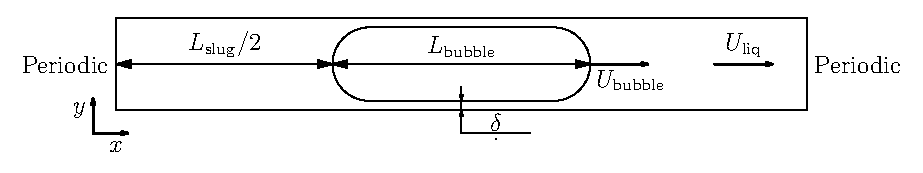
\includegraphics[width=\textwidth]{Figures/benchmark_hydro.eps}
\caption{Simplified sketch of the bubble train motion. Using periodic conditions for the velocity
field is natural, but needs validation for the mass transfer. \label{fig:benchmark:hydro}}
\end{figure}

To establish numerical procedures we performed multiphase simulations \cite{kuzmin-binary2d,kuzmin-binary3d} for the range of capillary numbers $Ca=0.1\div 1.0$ to extract bubble shapes. For this range of capillary numbers we are able to capture the bubble shape change and the change of hydrodynamic patterns. The mass transfer simulations were performed with different boundary conditions (open, periodic) and with a few unit cells ($1$ to $10$ unit cells).  The numerical approach we take is the lattice Boltzmann method, a relatively new CFD
competitor emerged during last $20$ years \cite{frisch,mcnamara,HJ,HSB}. During years the
method was applied to simulate not only hydrodynamic problems \cite{yu}, but as well multiphase
flows \cite{Shan-chen:extended,swift,gunstensen}, heat transfer
\cite{yuan-thermal,zhang-thermal}, ferrofluids \cite{dellar-ferro,kuzmin-aniso}.

The mass transfer problems in the lattice Boltzmann framework were mainly addressed in series of
works of Ginzburg and co-authors
\cite{ginzburg-main,ginzburg-boundary-conditions,ginzburg-saturated-flow}. However, all these works
are of general nature to simulate the advection-diffusion equation via the lattice Boltzmann
framework. In comparison, this work focuses on the application side as to establish the procedure of how to obtain the
volumetric mass transfer coefficients for bubble train flow. One should mention the work of
\citet{inamuro-scalar-boundary} about heat and mass transfers in the porous media and the work
of \citet{jos-mass} simulates lateral mixing in cross-channel flow. While two last works are focused
at the particular mass transfer problems, both problems are of homogeneous nature and do not
guide as how to obtain the mass transfer coefficient for non-homogenous problems.           

The paper is organized as follows. We start with definitions of the volumetric mass transfer coefficient and apply them 
for the bubble train flow to derive expressions to connect space and time domains. Then the lattice
Boltzmann model used to simulate mass transfer is presented followed by benchmarks. Finally,
numerical simulations of different boundary conditions and a few unit cells simulations for
different hydrodynamic patterns are presented to establish the thorough procedure to determine the
volumetric mass transfer coefficient. The comparison with analytical correlations is also presented. 

\section{Mass transfer definitions}
By the definition the mass transfer coefficient from the surface with the imposed constant
concentration $\cbubble$ is the following:
\beq
\label{eq:main:definition}
k_L=\frac{\dot{m}}{P \Delta C},
\feq
where $\dot{m}$ is the mass rate $\Bigl[\frac{kg}{s}\Bigr]$, $P$ is the area of the surface
$\Bigl[m^2\Bigr]$, $\Delta C$ is the concentration difference between the surface and the surrounding medium
$\Bigl[\frac{kg}{m^3}\Bigr]$. Therefore, $k_L$ has a dimension of velocity
$\Bigl[\frac{m}{s}\Bigr]$. Usually, the surrounding medium concentration is taken at the infinite distance
from the bubble. However, in the case of complicated geometries and non-homogeneous concentrations, 
the medium concentration can be the average concentration in the domain or the flux averaged
concentration at the inlet or outlet, etc. Thus, one needs to establish a thorough definition of the volumetric
mass transfer coefficient in the case of complex geometries and non-trivial hydrodynamic velocity patterns.

There are different methods to estimate the mass transfer coefficient $k_L$. We first examine the
theoretical definitions of the mass transfer in case of point mass sources.
\subsection{Point mass sources}
In what follows we will present three approaches to calculate point  mass transfer
coefficients (by point source we assume the source with the infinitesimally small surface area $P$):
\begin{enumerate}
\item
Let us look at the infinitesimal small domain of the volume $A \Delta x$ not
moving and with the point mass source.  Then the concentration difference can be found as $\Delta C =
\cstar -
C(t)$, where $\cstar$ is the imposed point source concentration, $C(t)$ is
the time dependent concentration, which do not depend on the location due to homogeneity. Therefore, one can write the time dependent ODE for the
concentration in the domain:
\beq
\dot{m}= A \Delta x \frac{\mathrm{d}C}{\mathrm{d} t} = k_L P (\cstar-C(t)), 
\feq
with the initial condition $C(0)=0$
The solution can be found by solving ODE:
\beq
C(t)= \cstar (1-\exp(-\vol t )), 
\feq
where $\vol$ is the volumetric mass transfer coefficient defined as:
\beq
\vol=k_L \frac{P}{A \Delta x}=k_L \frac{P}{V},
\feq
where $P$ is the source surface, $V$ is the unit cell volume.
\item
Let us predict mass transfer happening in moving with the velocity
$U$ liquid, see Fig. \ref{fig:moving:frame}. 
\begin{figure}[htb!]
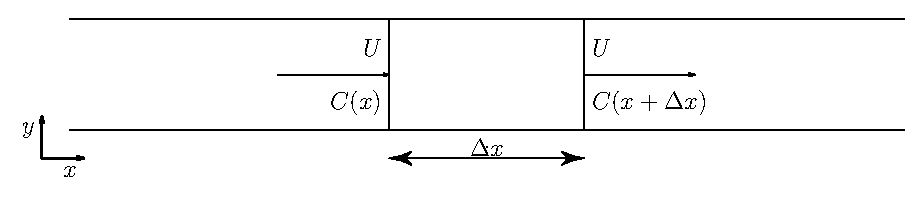
\includegraphics[width=\textwidth]{Figures/mass_transfer.eps}
\caption{The mass transfer in the moving liquid. \label{fig:moving:frame}}
\end{figure}

If one can assume that the mass point sources are distributed in the whole medium, then the mass accumulated in the unit volume $V=A \Delta x$ can be calculated as the difference of 
mass fluxes entering and leaving domain $U \bigl(C(x+\Delta x)-C(x)\bigr)$. The accumulated mass should be proportional
to the mass transfer coefficient:
\beq
U \bigl(C(x+\Delta x)-C(x)\bigr)=k_L P \bigl(\cstar-C(x)\bigr), 
\feq 
giving the same equation but only in the coordinate domain:
\beq
%\label{concentration:domain:coordinate}
C(x)= \cstar \Bigl(1-\exp\bigl(-k_L a \frac{x}{U} \bigr)\Bigr).
\label{main:mass:transfer:expression} 
\feq
Note that the concentration $C(x)$ does not depend on time. 

\item If one transfers to the frame moving with the liquid velocity $U$, then the situation will be
the same as in the first case. However, one can connect the time and spatial location with the
velocity $U$ ($t=\frac{x}{U}$) to obtain the same equation as in the case 2.
\end{enumerate}

\subsection{Bubble train}
In the application to the bubble train flow, it is useful to think of one bubble to be a point
source to make all considerations above valid. For example, the expression
(\ref{main:mass:transfer:expression}) was used in the experiments by
\citet{bercic-mass}. However, one should be accurate with the definition of velocities because two
different phases co-exist in the bubble train flow. Usually, one can take the velocity $U$ to be as
a bulk velocity or $U=\ugas+\uliq$, where $\ugas$ and $\uliq$ are liquid and gas
superficial velocities correspondingly. 

Thus, the experimental measurements are straightforward as measuring concentrations at
different
locations and calculating the volumetric mass transfer coefficient through the logarithmic
function. However, if one wants to analytically or numerically calculate the mass transfer coefficients, the
situation is much more complicated because of two phases presence and complicated bubble
geometry. As it was mentioned before depending on the capillary
number the mixing velocity pattern is different. Analytical approaches
\cite{irandoust,vanbaten-circular} assume that the
contributions from film and bubble caps can be calculated separately. However, one can see that
such 
an assumption (slug well mixed and the concentration is uniformly distributed over
the slug) usually overpredicts the mass transfer \cite{irandoust}. This happens since some tracer
concentration from film is mixed with the slug and increases the overall concentration in the slug. Thus, it decreases the mass transfer from bubble caps.
Therefore, all estimations for the analytical mass transfer coefficient calculation  do not account for mutual mass
transfer from
neighbouring bubbles.

Another issue is that if the bubble is long enough then the film saturates with the tracer
concentration and its influence on mass transfer can be negligible \cite{vanbaten-circular}.
Mixing patterns of the film and liquid slugs are of great importance for the analytical
estimation of mass transfer \cite{yue-mass}. However, the assumptions usually taken for the
mass transfer calculation are small capillary number and certain mixing patterns which help to
estimate the mass transfer using the penetration theory of \citet{higbie}.

In comparison with analytical calculations and simplifications, the numerical approach can take into
the account the complicated mixing patterns and geometries. However, there are challenges as to
mimic the continuous picture like moving with bulk velocity $U=\ugas+\uliq$ reacting medium as it is seen in
experiments. Thus, the questions indicated in Section \ref{intro}, as the choice of the
characteristic concentration, the choice of boundary conditions, arise. Next
section gives more details about numerical simulations.
 
\subsection{Numerical simulations}
\label{section:cases}
Ideally one needs to mimic the continuous picture as it is seen in experiments. Thus, mass transfer simulations for a number of unit cells is needed. As it was indicated above there are
two approaches towards it - either to simulate
the bubble train and then to measure concentration along the pipe, Eq.
\ref{main:mass:transfer:expression}, or to transfer to the reference frame moving with the bulk
velocity $U$ and conduct same measurements. However, both methods do require a tracking of
moving bubbles which is complicated from the numerical point of view. Therefore, one needs to come
up with simple smaller domain calculations of the mass transfer coefficient, which mimic the
continuous picture with infinite numbers of the bubbles closely. 

To avoid complications with moving grids, our
approach is to simulate mass transfer in the reference frame moving with the bubble. Therefore, one
needs to examine  Eq.
\ref{main:mass:transfer:expression} more closely. 

We perform simulations in the frame moving with the bubble (velocity
$\ububble$), that the bubble position stands steady. The bubble velocity $\ububble$ is
different from the bulk velocity $U=\ugas+\uliq$. In this case one needs to perform a coordinate $x$
variable change:
\beqal
\label{theor:average:concentration:time}
&x(t)=\ububble t\\
&\overline{C(x)}=\cstar \Bigl(1-\exp\bigl(-\vol \frac{x}{\ugas+\uliq}\bigr)\Bigr)\\
&\langle C(t)\rangle=\cstar \Bigl(1-\exp\bigl(-\vol\, t \frac{\ububble}{\ugas+\uliq}\bigr)\Bigr),
\feqal
where $\langle C(t)\rangle$ is the characteristic concentration averaged in space, $\overline{C(x)}$ is averaged in time concentration at location $x$. 
%The geometry is not one-dimensional and one needs the characteristic concentration
%to be only as a function of time. 
One can have different choices of
$\langle C(t) \rangle$ as the averaged in whole domain concentration or inlet/outlet averaged in
space concentrations used in works \cite{vanbaten-circular,kreutzer-overview}.  
%Note that $C(x)$ is not averaged in time as $\overline{C(x)}$ since $C(x)$
%ideally should not depend on time. 
Therefore, one can obtain the volumetric mass transfer coefficient through the concentration averaged in space:
\beqal
\label{theor:one:concentration:time}
&\vol\, t \frac{\ububble}{\ugas+\uliq}=\ln \frac{\cstar}{\cstar-\langle C(t)\rangle}\\
&\volnondim=\frac{\lunit}{\ububble t}\ln \frac{\cstar}{\cstar-\langle C(t) \rangle},
\feqal
where the parameter $\vol \frac{\lunit}{\ugas+\uliq}$ is non-dimensional. One can also measure the
volumetric mass transfer coefficient from concentrations given at times $t_1$ and $t_2$:
\beq
\label{theor:continuous:mass:transfer}
\volnondim=\frac{\lunit}{\ububble
(t_2-t_1)}\ln\frac{C^{*}-\langle C(t_1) \rangle}{C^{*}-\langle C(t_2) \rangle}.
\feq
Expressions (\ref{theor:average:concentration:time}) and (\ref{theor:continuous:mass:transfer}) are
cornerstones of the present work. The main questions arisen in the present work are to define the
characteristic concentration $\langle C(t) \rangle$ and  boundary conditions to calculate a proper
volumetric mass transfer coefficient
$\vol$. 
  
Four possible scenarios of  numerical simulations are examined in this work: 
\begin{enumerate}
\item % The bubble train multiphase simulations are conducted by applying periodic boundary
%conditions \cite{kuzmin-binary2d,kuzmin-binary3d}. 
%One
%can make an assumption of same boundary
%conditions applied to the tracer concentration to simulate mass transfer. 
One unit
cell is simulated with
periodic boundary conditions, see Fig. \ref{fig:benchmark}. 
Thus, no tracer leaves a
domain like for the plug flow. 
%From the physical point of view this case resembles the mass transfer for small Capillary numbers
%$Ca<0.1$.  The liquid slug is well mixed and one have a homogeneous concentration in the unit
%cell, i.e. the outlet and the inlet concentrations are close. 
Though easier to implement, it rises certain criticism
about the inlet concentration to be equal to the outlet concentration. As it was discussed, in experiments there is the concentration difference between the inlet and
 the outlet.

The volumetric mass transfer coefficient is calculated by Eq. \ref{theor:one:concentration:time}.
The
characteristic concentration $\langle C(t) \rangle$ required for the volumetric mass
transfer coefficient, Eq.
\ref{theor:one:concentration:time}, is taken as the average concentration in the domain:
\beq
\label{average:concentration:definition}
C(t)=\frac{\int_{liquid}{C \mathrm{d}V}}{\int{\mathrm{d}V}}.
\feq
\begin{figure}[htb!]
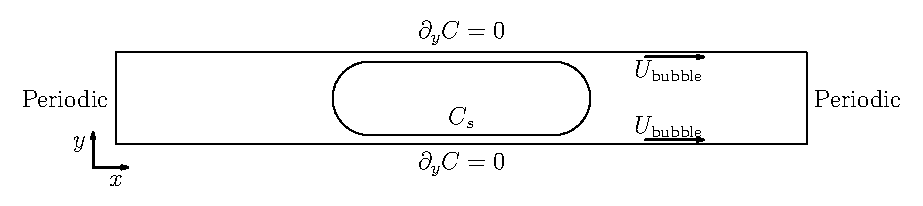
\includegraphics[width=\textwidth]{Figures/benchmark_middle.eps}\\
\caption{The two-dimensional benchmarks for the  the mass transfer
coefficient (bottom) for the bubble located near the entrance (top) and at the middle of the domain
(bottom). \label{fig:benchmark}}
\end{figure}
\item The second approach is to apply periodic boundary conditions as in the first case but the characteristic concentration is taken as the inlet/outlet
concentration \cite{vanbaten-circular}:
\beqal
&\langle \cinlet(t) \rangle=\frac{\int{U(y) C(0,y,t) \mathrm{d}y}}{\int{U(0,y) \mathrm{d}y}}\\
&\langle \coutlet(t) \rangle=\frac{\int{U(y) C(\lunit,y,t) \mathrm{d}y}}{\int{U(\lunit,y)
\mathrm{d}y}}\\
&\cinlet(\bm{x},t)=\coutlet(\bm{x},t),\,\text{due to periodicity}.
\feqal
Therefore, the assumptions  of this approach is
that the difference between inlet and outlet is not
considerably large and the tracer is well mixed in the slug. Thus, the inlet or outlet
concentrations equal to the average concentration. 

\item
The approach of \citet{vanbaten-circular} is examined. Periodic boundary conditions were used. The work \cite{vanbaten-circular}
calculates the mass transfer coefficient as the gain of the mass in the system
divided by the concentration difference
multiplied on the surface area:
\beq
\vol=\frac{\dot{m}}{P \Delta C}\frac{P}{V}=\frac{\dot{m}}{V (\cstar-\langle C(t) \rangle)},
\feq
where mass difference in the domain can be calculated as:
\beq
\dot{m}=\frac{m_2-m_1}{t_2-t_1}=\frac{\int_{liq}{C(\bm{x},t_2)\mathrm{d}V}-\int_{liq}{
C(\bm{x},t_1)\mathrm { d } \bm{x}} } {
t_2-t_1 }.
\feq
In the approach of \citeauthor{vanbaten-circular} the inlet and outlet concentrations were taken as the
characteristic concentration $\langle C(t) \rangle $.

%\item 
%The approach of the opened boundaries was examined, see Fig. \ref{fig:benchmark:jos}. At the inlet
%and outlet boundaries the diffusion flux was imposed to be zero, $\frac{\partial C}{\partial x}=0$.
%The characteristic concentration was taken as the average concentration in the whole domain.
%\begin{figure}
%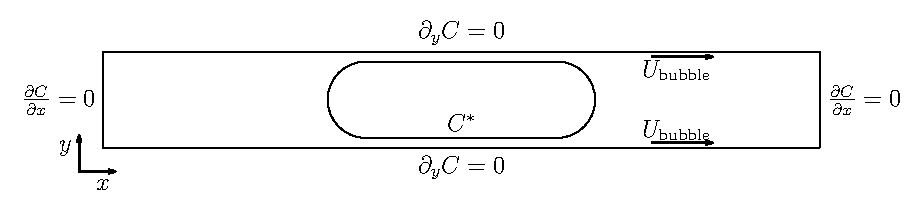
\includegraphics[width=\textwidth]{Figures/benchmark_jos.eps}
%\caption{The numerical mass transfer benchmark with open boundaries. The mass transfer is
%calculated according to Eq. \ref{theor:average:concentration:time} with the characteristic
%concentration accoring to Eq. \ref{average:concentration:definition}. \label{fig:benchmark:jos}}
%\end{figure}
\item 
The last approach to be examined in this paper is the simulation of a few unit cells, see Fig. \ref{fig:benchmark:alot}. This situation corresponds to the simulation of the
bubble train head, after injecting to the pipe and travelling along the pipe. One can see that this
situation corresponds most to the experimental picture. By simulation of a certain number of the
bubble train head, the influence of the boundaries can be
diminished. In this case, there is no ambiguity in the choice of the
characteristic concentration. The average concentration of any unit cell far away from boundaries will be governed
by Eq.
\ref{theor:continuous:mass:transfer}. This simulation statement is of most correspondence to
experiments and should give right answer. However, one of the
disadvantages is to simulate a certain number of unit cells ($1$ to $10$ in this case), thus
increasing a computational
burden.
\begin{figure}[htb!]
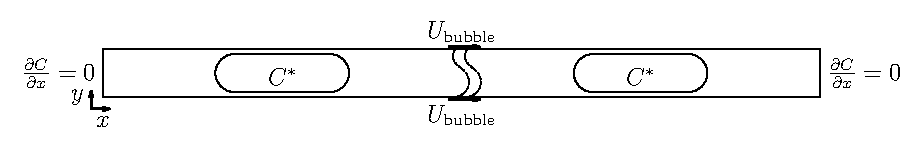
\includegraphics[width=\textwidth]{Figures/benchmark_alot.eps}\\
\caption{Benchmark for a lot of units. \label{fig:benchmark:alot}}
\end{figure}
\end{enumerate} 

One can notice that all examined cases are extreme cases of one equation:
\beq
\label{main:main:main}
\vol=\frac{\dot{m}-\int{\coutlet(t) u(\lunit,y)\mathrm{d}y}+\int{\cinlet(t) u(0,y)\mathrm{d}y}}{V
\Delta C}, 
\feq
where $\Delta C=\cstar-\langle C(t) \rangle$ with $\langle C(t) \rangle$ to be the average
concentration in whole liquid domain, $\dot{m}$ is the mass gain in the domain,$\int{\cinlet u(0,y) \mathrm{d}y}$ and $\int{\coutlet u(\lunit,y)\mathrm{d}y}$ are inlet/outlet mass fluxes. Eq. \ref{main:main:main} describes the mass
balance: whatever was generated by the bubble surface equals to the mass domain change minus
whatever left domain plus whatever entered domain. 

Periodic boundary condition is the extreme
limiting case of Eq. \ref{main:main:main}: 
\beqstar
\int{\coutlet(t)
u(\lunit,y)\mathrm{d}y}=\int{\cinlet(t) u(0,y)\mathrm{d}y}. 
\feqstar
Then the mass change in the domain is
only because of the generating bubble surface. However, to calculate the mass transfer coefficient one needs to have characteristic concentration  $\langle C(t) \rangle$ and mass gain $\dot{m}$ which do require the storage of time and space information.

Another limiting case (will be shown later) is hydrodynamic pattern change $Ca>0.7$. The mass accumulation rate equals zero in this case, $\dot{m}=0$. One can use only spatial information to calculate the mass transfer coefficient, i.e. $\int{\cinlet(t) u(0,y)
\mathrm{d}y}$ and $\int{\coutlet(t) u(\lunit,y)\mathrm{d}y}$ require only space information. 

Before we examine all the test cases above, the lattice Boltzmann mass transfer
benchmarks will be presented. 

\section{Validation}
For analytical expressions the problem of the mass transfer can be decomposed to the following
parts: the mass transfer from two circumferences and the mass transfer from the film. We will
examine
these problems with the help of the lattice Boltzmann method and compare them against analytical
solutions. The next sections will present the lattice Boltzmann method and a few benchmarks.

\subsection{TRT $D2Q9$ model}
The lattice Boltzmann equation (LBE) operates on a square/cubic grid representing the
physical domain. It utilizes
probability distribution functions (also known as particle populations)
containing information about
macroscopic variables, such as fluid density and momentum. LBE consists of
two parts: a local collision step, and a propagation step which transports
information from one node to another along some 
directions specified by the discrete velocity set.
The LBE is typically implemented as follows:
\begin{equation}
\label{standard:implementation}
\begin{aligned}
&f_i^{*}(\bm{x},t)= f_i(\bm{x},t)-\omega \bigl(f_i(\bm{x},t)-eq_i(\bm{x},t)\bigr),&&\text{
collision step}\\
&f_i(\bm{x}+\bm{c_i},t+1)=f_i^{*}(\bm{x},t),&&\text{ propagation step}, 
\end{aligned}
\end{equation}
where $f_i$ is the probability distribution function in the direction $\bm{c_i}$,
 $f_i^{eq}$ is the equilibrium probability distribution function, $\omega$ is the
relaxation parameter. Collision operator, $-\omega \bigl(f_i- f_i^{eq}\bigr)$ is so-called BGK
collision operator \cite{bgk}. However, the approach to be used here is the TRT
(two-relaxation-times) collision operator \cite{ginzburg-main,ginzburg-saturated-flow}. In
comparison with the widely used BGK collision operator, TRT collision operator has better accuracy
for diffusion and convection fluxes, and larger range of parameters where the LBM scheme is stable.

The TRT collision operator \cite{ginzburg-boundary-main}
decomposes the populations and the equilibrium
distribution into the symmetric and antisymmetric parts:
\begin{equation}
\label{trtdecomp}
f^{\pm}_i=\frac{f_i\pm f_{\bar{i}}}{2}\;,\; 
{eq_i}^{\pm}=\frac{eq_i\pm eq_{\bar{i}}}{2}\;,
\end{equation}
where $\bar{i}$ is the opposite direction to the $i$-th direction.
The collision is performed with two independent relaxation rates for 
symmetric and antisymmetric modes:
\begin{equation}
\label{trt}
\begin{aligned}
&f_i^{*}(\bm{x},t)=f_i(\bm{x},t)-\omegaplus (f_i^{+} - eq_i^+)-\omegaminus
(f_i^{-} -
eq_i^-)\\
&f_i(\bm{x}+\bm{c_i},t+1)=f_i^{*}(\bm{x},t).
\end{aligned}
\end{equation}
Note that the BGK collision operator is the particular subclass of the TRT relaxation operator with
$\omegaplus=\omegaminus$. In comparison with the BGK collision operator,
the TRT collision operator has the additional degree of freedom. Thus, the TRT operator then
introduces
the free parameter
$\Lambda=\Bigl(\frac{1}{\omegaplus}-\frac{1}{2}\Bigr)\Bigl(\frac{1}{\omegaminus}-\frac{1}{2}
\Bigr)$. 
This free parameter controls the effective location of the bounce-back
walls \cite{ginzburg-multireflection}, second-order accuracy of
boundary \cite{ginzburg-boundary-main} and interface schemes \cite{ginzburg-discontinious}, 
spatial accuracy \cite{ginzburg-recurrence,servan-trt-stability},
consistency \cite{ginzburg-brinkman} and, to some extent,
stability \cite{kuzmin-stability-optimal,kuzmin-d1q3,servan-trt-stability}.
In particular, $\Lambda=\frac{1}{4}$ achieves the optimal stability for the
linear advection-diffusion isotropic equation \cite{kuzmin-stability-optimal}. 

The parameters $\omegaplus$, $\omegaminus$ and $eq_i$ fully define the lattice Boltzmann
procedure. The two-dimensional nine velocities LBM $D2Q9$ we used in this work is defined on the set
of lattice
velocities with coordinates:
\beqal
&c_{ix}=\{0,1,0,-1,0,1,-1,-1,1\},\text{ for } i=0\dots8\\
&c_{iy}=\{0,0,1,0,-1,1,1,-1,-1\},\text{ for } i=0\dots8\,.
\feqal

The equilibrium functions for $D2Q9$ TRT model are represented as \cite{kuzmin-stability-optimal}:
\begin{equation}
\begin{aligned}
&eq_i^{+}=eq_i^{(m)}+g^{(u)} eq_i^{(u)}\\
&eq_i^{(m)}=t_i^{(m)} c_e+ eq_i^{(a)}\\
&eq_i^{(u)}=t_i^{(u)} \frac{u_x^2+u_y^2}{2}+\frac{u_x^2-u_y^2}{4} p_i^{(xx)}+g_{xy}^{(u)}\frac{u_x
u_y}{4} p_i^{xy}\\
&eq_i^{(a)}=\frac{K_{xx}-K_{yy}}{4} p_i^{xx}+\frac{D_{xy}}{4} p_i^{(xy)},
\end{aligned}
\end{equation}
where $K_{xx,yy,xy}$ are proportional to components of the diffusion tensor,
$c_e=\frac{K_{xx}+K_{yy}}{2}$, parameters $g^{(u)}$ and $g^{u}_{xy}$ are either zero or one (see
below), the tensor $p_i^{(xx)}=c_{ix}^2-c_{iy}^2$, the tensor $p_i^{(xy)}=c_{ix} c_{iy}$, the
weights
$t_i^{(u,m,a)}$ can be chosen based on stability criteria. Though not the best set of weights for
stability \cite{kuzmin-stability-optimal}, but the most spread set of weights, so called
``hydrodynamic`` weights, was chosen:
\begin{equation}
t_i^{(u)}=t_i^{(m)}=t_i^{(a)}=\Bigl\{0,\frac{1}{3},\frac{1}{3},\frac{1}{3},\frac{1}{3},\frac{1}{12},
\frac {1}{12},\frac{1}{12},\frac{1}{12}\Bigr\}
\end{equation}
 
It can be shown through the Chapman-Enskog procedure \cite{chapman}, that the simple update rule
with the equilibrium function presented above restores the anisotropic
advection-diffusion equation:
\beq
\partial_t C+ \partial_{\alpha} C u_{\alpha}=\partial_{\alpha\beta} D_{\alpha\beta} C,
\feq
where $D_{\alpha\beta}=\Bigl(\frac{1}{\omegaminus}-\frac{1}{2}\Bigr)K_{\alpha\beta}$
with the
following diffusion tensor:
\begin{equation}
D_{\alpha\beta}=
\begin{pmatrix}
D_{xx} + \Bigl(\frac{1}{\omegaminus}-\frac{1}{2}\Bigr)(g^{(u)}-1) u_x^2 &
D_{xy}+\Bigl(\frac{1}{\omegaminus}-\frac{1}{2}\Bigr)(g_{xy}^{(u)}-1)u_x u_y\\
D_{xy} + \Bigl(\frac{1}{\omegaminus}-\frac{1}{2}\Bigr)(g_{xy}^{(u)}-1) u_x u_y&
D_{yy}+\Bigl(\frac{1}{\omegaminus}-\frac{1}{2}\Bigr)(g^{(u)}-1) u_y^2. 
\end{pmatrix}
\end{equation}
We want to resolve the isotropic advection-diffusion equation, $D=D_{xx}=D_{yy}$ or
$K=K_{xx}=K_{yy}$, with the non-diagonal diffusion tensor components to be zero $D_{xy}=0$. In
comparison with the $D2Q5$ model, with the $D2Q9$ it is
possible to cancel the numerical diffusion by the proper choice
of the equilibrium functions, i.e. $g_{xy}^{(u)}=g^{(u)}=1$.  The particular choice of parameters
used in simulations is $c_e=\frac{1}{3}$, $\Lambda=\frac{1}{4}$. Thus, the diffusion coefficient $D$
is matched through $\omegaminus$, i.e. $D=c_e
\Bigl(\frac{1}{\omegaminus}-\frac{1}{2}\Bigr)=\frac{1}{3}(\frac{1}{\omegaminus}-\frac{1}{2}\Bigr)$.
 Free relaxation parameter $\omegaplus$ can be found through $\Lambda$. For particular
choice $\Lambda=\frac{1}{4}$ (the optimal stability parameter), $\omegaplus$ can be found easily as
 $\omegaplus=2-\omegaminus$.  

%Fig. \ref{stability:d2q9} shows the stability limits for the $D2Q9$
% model $c_e$ against $U^2=u_x^2+u_y^2$ for two particular choices.
% \begin{figure}[htb!]
% 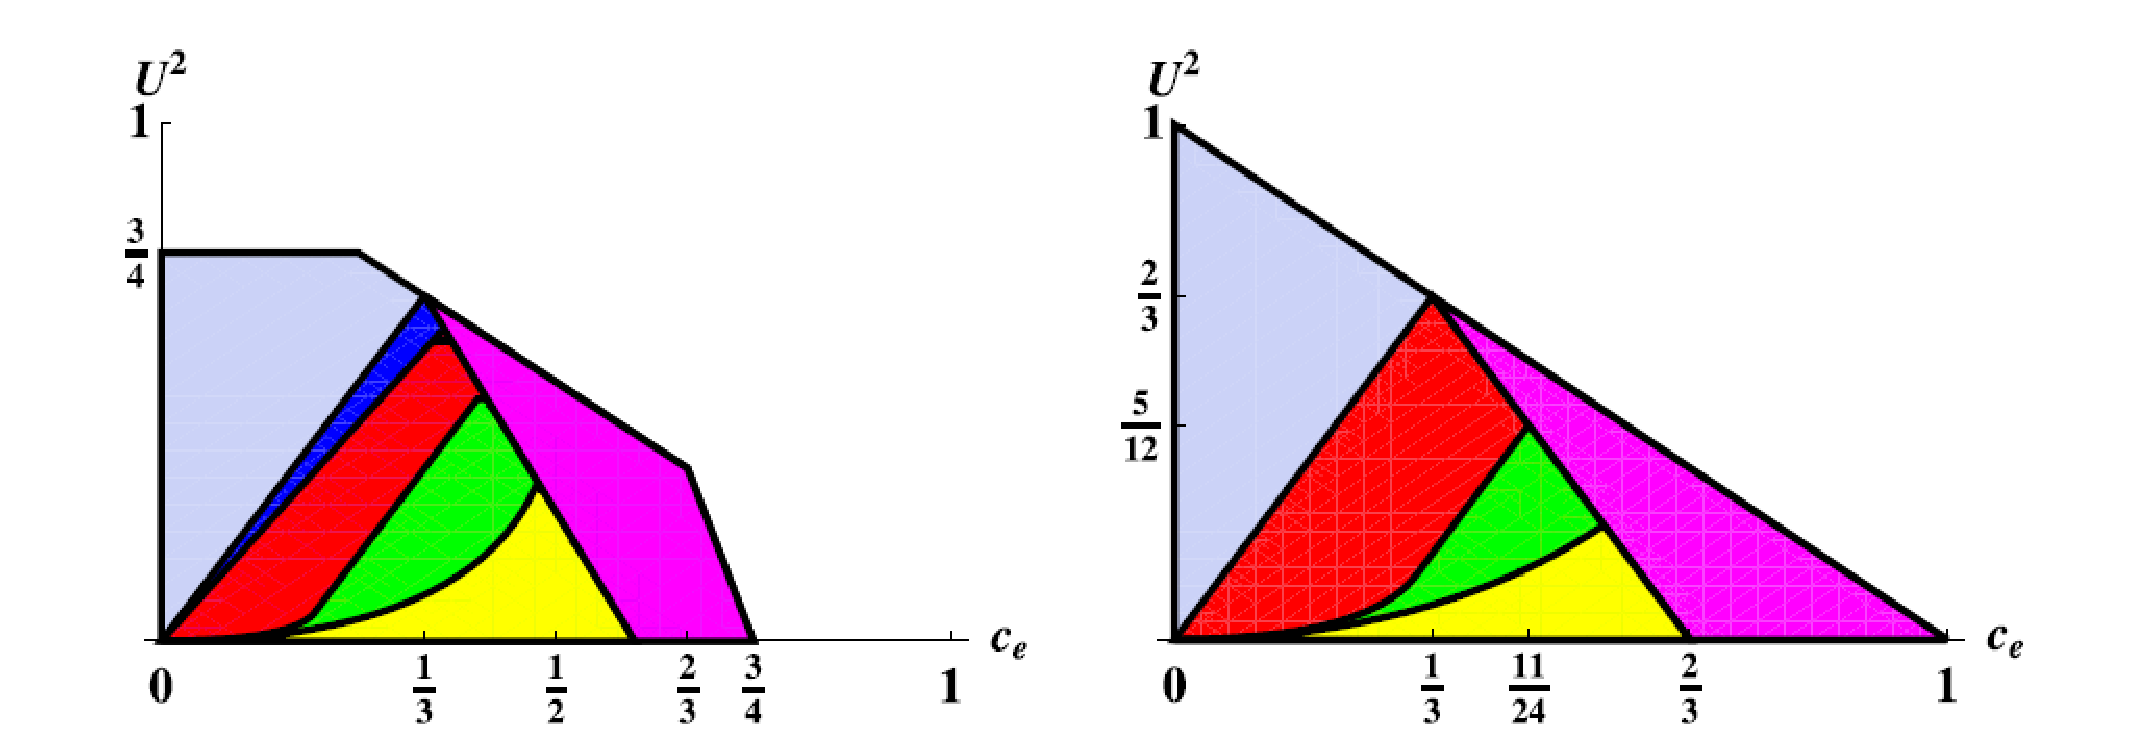
\includegraphics[width=\textwidth]{Figures/d2q9_stability.eps}
% \caption{The stable sub-domains of the $D2Q9$ schemes ($\Lambda=\frac{1}{4}$)
% are plotted for standard (hydrodynamic) weights (left) and uniform weights (right, not mentioned
%here) when the
% numerical diffusion is removed, partially or completely. For particular choice used in this work
%(hydrodynamic weights, $c_e=\frac{1}{3}$, left picture), the achieved stable velocity is
%$u_x^2+u_y^2\leq\frac{2}{3}$. The non-negativity of populations (green+yellow) is for BGK
%stability. One can see that the achieved maximum stable velocity is twice smaller $u_x^2+u_y^2\leq
%\frac{1}{3}$ for the BGK collision operator.The proper choice of weights can
% allow to obtain  total triangle $0 \leq u_x^2+u_y^2 \leq 1- c_e$ (the
% uniform weights only).
% \label{stability:d2q9}}
% \end{figure}

Boundary conditions for the mass transfer used in this work are all of Dirichlet type. We validated
two types of boundary conditions: Inamuro boundary conditions \cite{inamuro-scalar-boundary} and
pressure anti bounce-back boundary conditions \cite{ginzburg-multireflection}. However, the
simulation results presented in this work are only pressure anti bounce-back due to its simplicity
to handle any complicated type of boundary:
\beq
\label{antibb}
f^{*}_{B,i}=-f^{*}_{F,\bar{i}} + 2 eq^+(\cstar,\bm{u}),
\feq
where $\cstar$ is the concentration to be imposed at the surface, $\bm{u}$ is the surface velocity,
$i$ is the direction number pointing to the domain (unknown) located at the boundary surface $B$,
$\bar{i}$ is the direction number opposite to $i$ and is located at the fluid $F$ specifically that
$B$ is located at the location $F+c_i$. 

Note that the parameters of the lattice
Boltzmann scheme are connected with the physical parameters only through the non-dimensional
numbers governing the physics of the problem. In our case, this number is the Peclet number, $Pe=\frac{\ububble L}{D}$.
Therefore, one can substitute any quantity, i.e.
$\ububble$ in the lattice Boltzmann units as soon as the
Peclet number is the matched in physical space and numerical simulations. This fact that $\ububble$
can be chosen arbitrarily is extremely useful in the context of numerical simulations, since it can
increase the time step, or decrease the computational demand by order of magnitude to obtain
meaningful results. This point will be extensively covered later. 

Next section will cover LBM benchmarks that resemble the mass transfer problem from a bubble, as as
mass transfer from the film  and circumferences.

\subsection{The radial case}
The case to be examined here is the mass transfer from the stair-case boundary forming a circle. It
can be
prescribed by the following system of equations:
\beq
\begin{aligned}
&\partial_t C(r,t)=\frac{1}{r}\partial_r r \partial_r C(r,t)\\
&C(a,t)=C_0,\,C(r,0)=C_{init}
\end{aligned}
\feq 
The solution is represented as \cite{chemical-correlations}:
\beq
\frac{C(r,t)-C_{0}}{C_{init}-C_{0}}=\sum_{n=1}^{\infty}{\frac{2}{\mu_n
J_1(\mu_n)}\exp\Bigl(-\mu_n^2 \frac{D t}{a^2} \Bigr)J_0(\mu_n \frac{r}{a})},
\feq
where $\mu_n$ is the $n$-th zero root of the $0$th order Bessel polynomial $J_0(\mu_n)=0$. Some of
the corresponding roots are as follows: $\mu_1=2.4048$,$\mu_2=5.5201$,$\mu_3=8.6537$,
$\mu_4=11.7915$,$\mu_5=14.9309$.
By taking initial concentration to be $0$, one can obtain the following solution:
\beq
C(r,t)=C_0 \Biggl(1 - \sum_{n=1}^{\infty}{\frac{2}{\mu_n
J_1(\mu_n)}\exp\Bigl(-\mu_n^2 \frac{D t}{a^2} \Bigr)J_0(\mu_n \frac{r}{a})}\Biggr).
\feq

The solution depends only on the non-dimensional time: $\tau=\frac{D t}{a^2}$. The domain size was $129\times 129$ with the circle radius $a=40$ units. Some examples for
different diffusion coefficients are presented in Fig.\ref{fig:cylinder:benchmark}.
\begin{figure}[htb!]
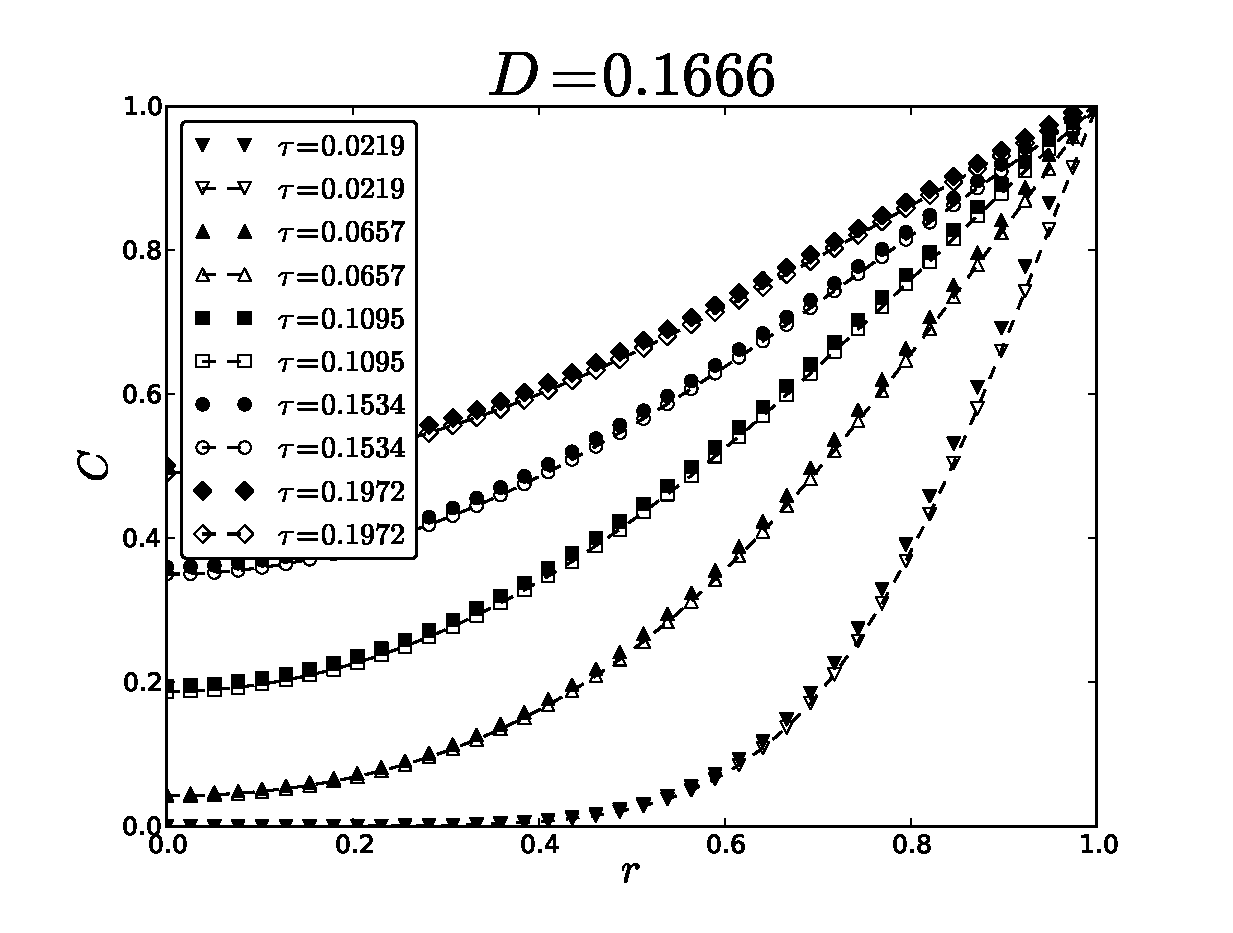
\includegraphics[width=0.5\textwidth]{Figures/cylinder1666.eps}
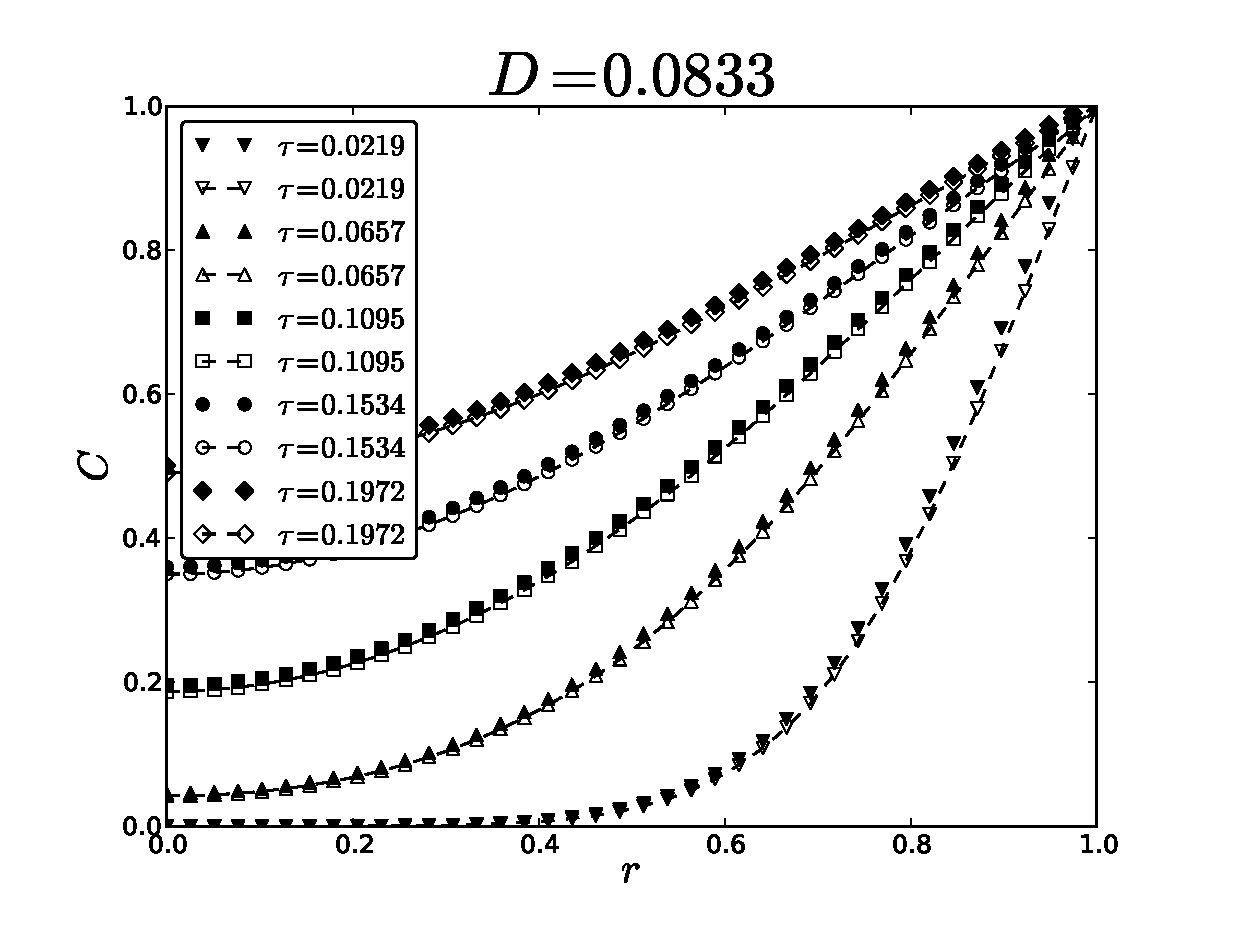
\includegraphics[width=0.5\textwidth]{Figures/cylinder0833.eps}\\
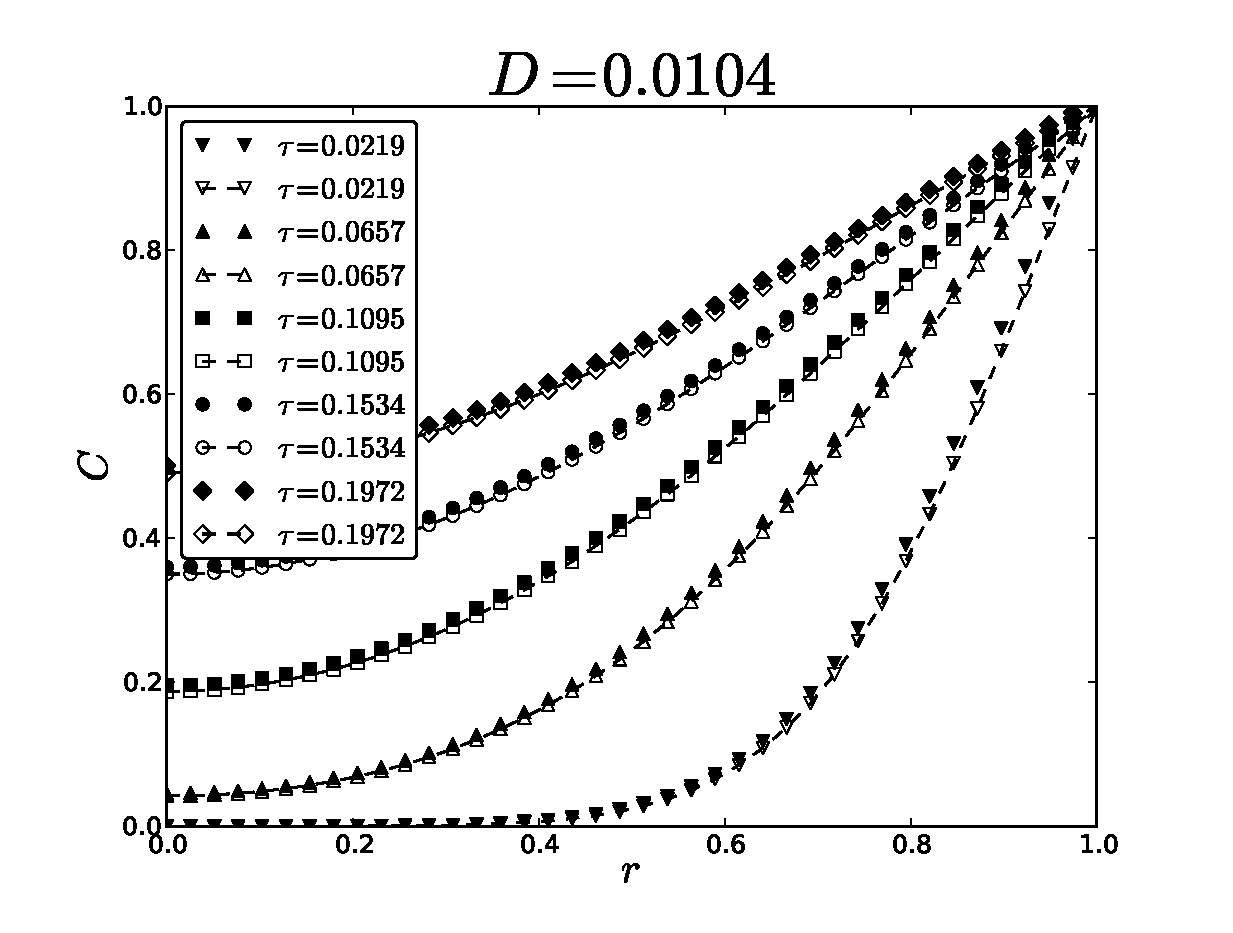
\includegraphics[width=0.5\textwidth]{Figures/cylinder0104.eps}
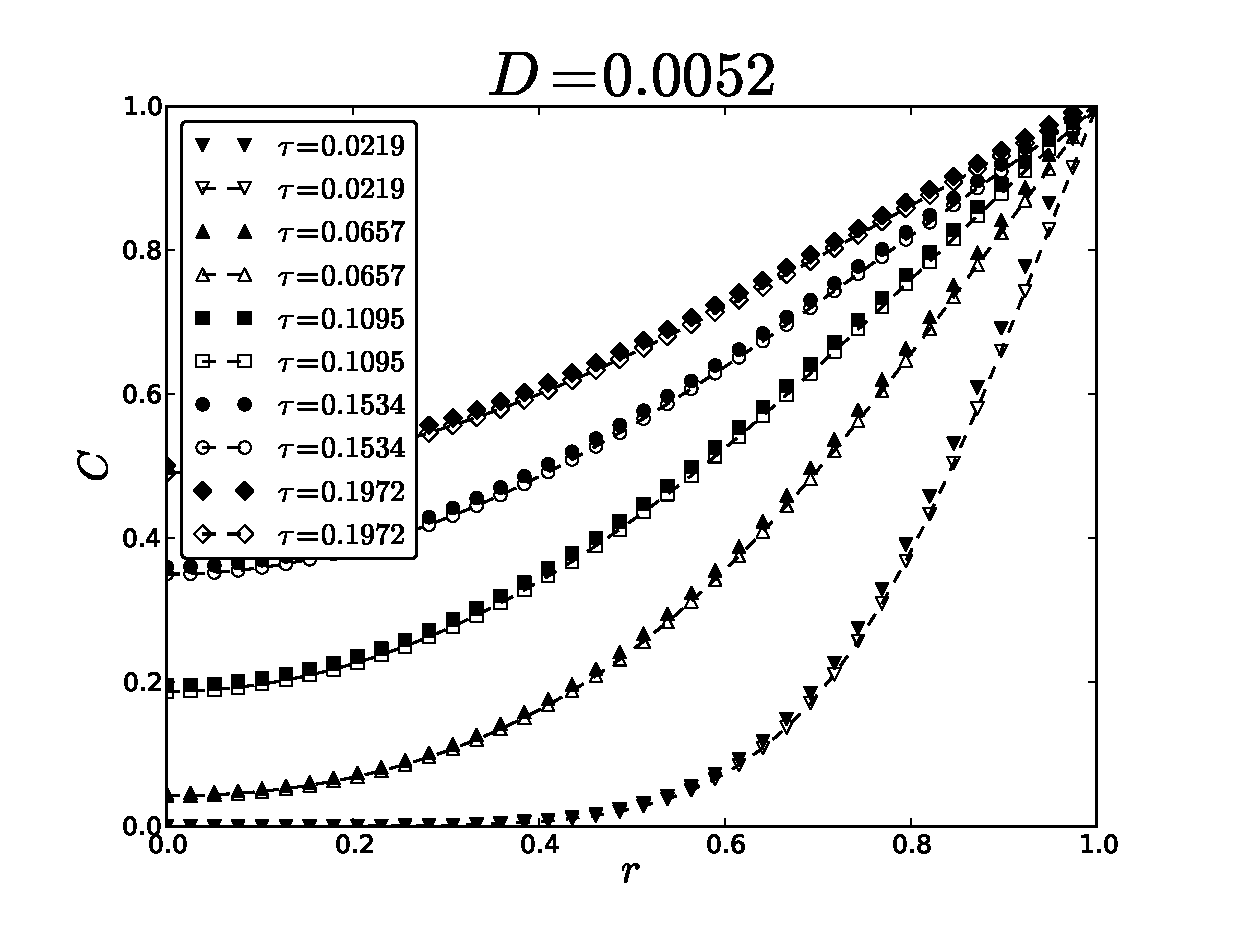
\includegraphics[width=0.5\textwidth]{Figures/cylinder0052.eps}\\
\caption{Profiles for different diffusion parameters varied with $\omegaminus$. One can see that the
diffusion from curved boundaries is captured
accurately \label{fig:cylinder:benchmark}. $x$ is the distance from the center.}
\end{figure}

\subsection{Parabolic profile with the velocity zero gradient at the wall}
The problem is defined in terms of PDE as follows: 
\beq
\begin{aligned}
&\frac{\partial C}{\partial x} U(y)=D\frac{\partial^2 C}{\partial y^2}\\
&C(0,y)=C_0,\, C(x,0)=\cstar,\, \frac{\partial C}{\partial y }(x,\delta)=0\\
&U(y)=U_0 \Bigl(\frac{y}{\delta}\Bigr)^2.
\end{aligned}
\feq
The procedure to solve this PDE is presented in Appendix \ref{appendix:zero:gradient}:
\beq
\label{analytical:solution:zero:gradient}
\begin{aligned}
&C(x,y)=\cstar+\sum_{m}{C_m
\sqrt{\frac{y}{\delta}}J_{\frac{1}{4}}\Bigl(\frac{m^2}{2}\frac{y^2}{\delta^2}\Bigr)\exp\Bigl(-\frac{
m^4 } { Pe }
\frac { x }{\delta}\Bigr)}\\
&C_m = (C_0-\cstar) \frac{\int_{\xi=0}^{1}{\xi^{5/2} J_{\frac{1}{4}}\Bigl(\frac{m^2
\xi^2}{2}\Bigr)\mathrm{d}\xi}}{\int_{\xi=0}^{1}{\xi^3 J_{\frac{1}{4}}^2\Bigl(\frac{m^2
\xi^2}{2}\Bigr)\mathrm{d}\xi}}
\end{aligned}
\feq
Fig. \ref{fig:parabolic:zero:gradient} shows the steady-state contours comparison between the
analytical and the simulation with the Anti Bounce-Back conditions used to impose constant
concentrations at the wall $\cstar=1$ and the inlet $C_0=0$. The grid used in the simulation is
$80\times1600$. Parameter $\omegaminus=1.8$ implies the diffusion coefficient to be
$D=\frac{1}{3}\Bigl(\frac{1}{\omega}-\frac{1}{2}\Bigr)=0.0185$.  
\begin{figure}[htb!]
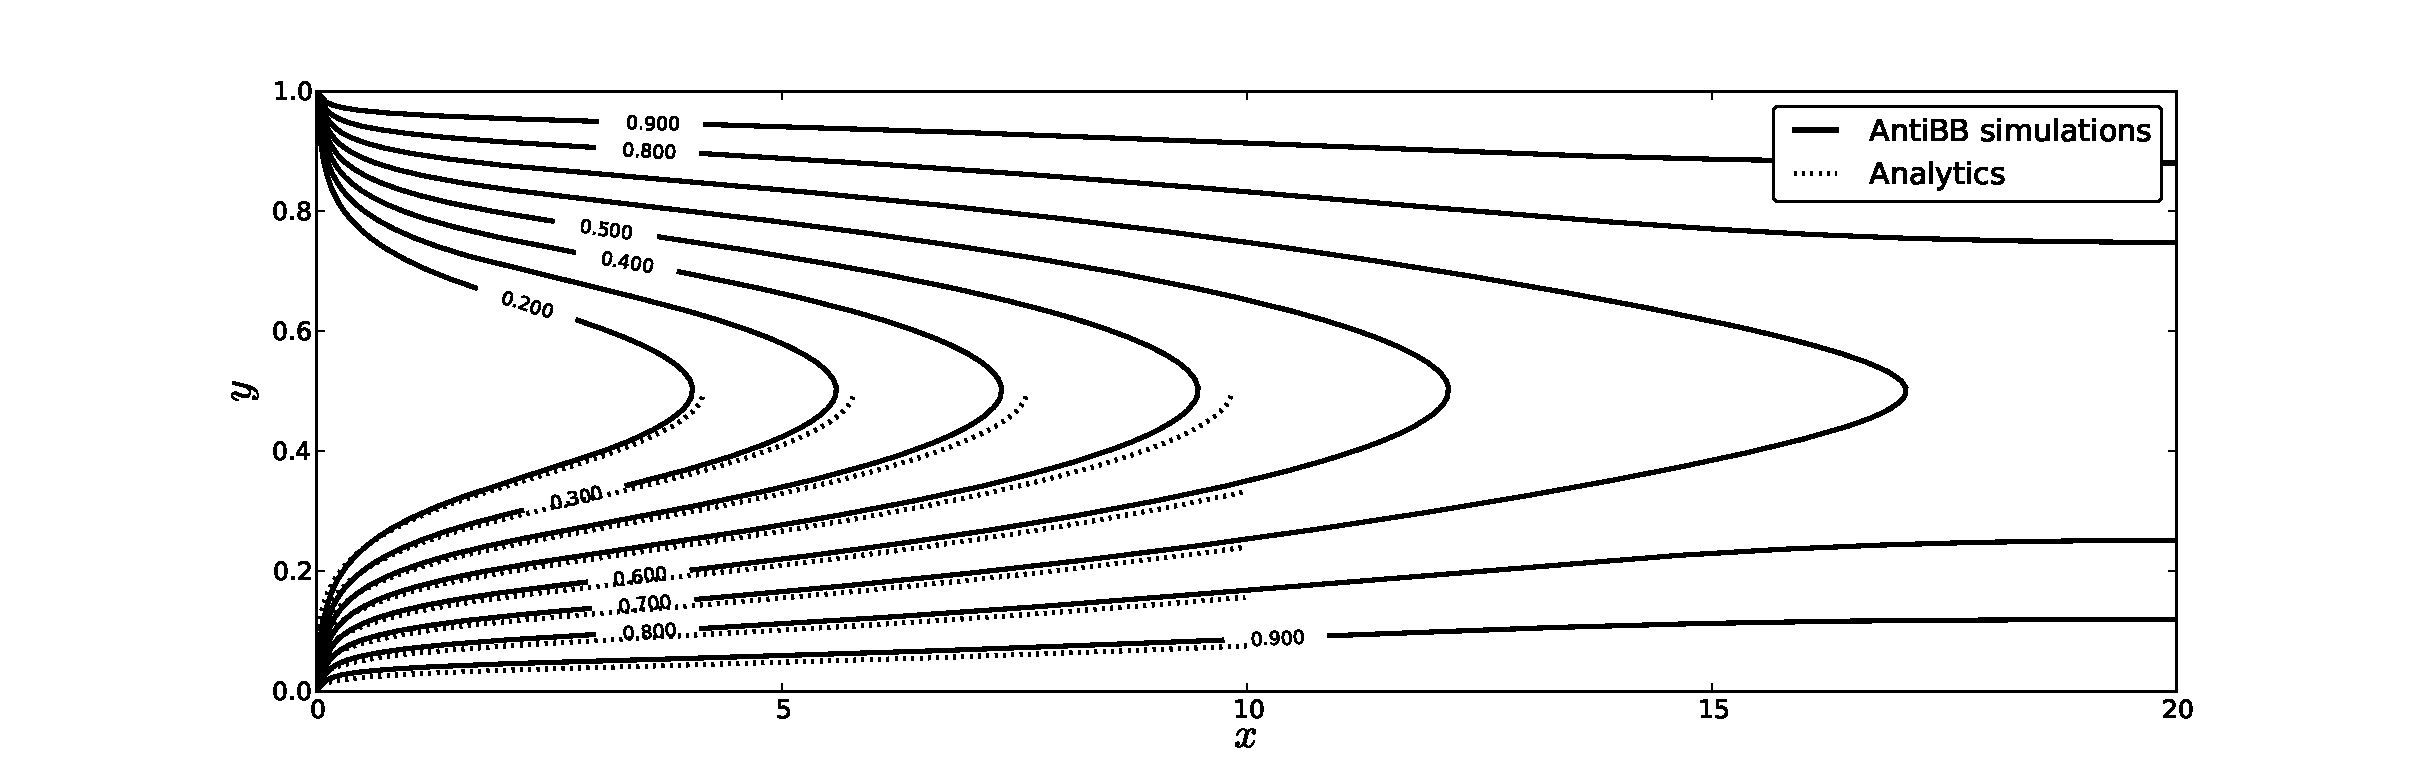
\includegraphics[width=\textwidth]{Figures/parabolic_profile_zero_gradient_comparison.eps}
\caption{Comparison with the analytical concentration contours, Eq.
\ref{analytical:solution:zero:gradient}, for the diffusion coefficient $D=0.0185$. Simulation was
performed on grid $80\times 1600$. The constant concentration is imposed with the
anti bounce-back conditions, Eq. \ref{antibb}. Coordinate $x$ and $y$ are non-dimensionalized on
the height of the channel. $\delta=H/2$ is the half of the channel height
\label{fig:parabolic:zero:gradient}}
\end{figure}
 
\subsection{Poiseulle velocity parabolic profile}
The problem we want to address can be formulated through the following PDE:
\beq
\begin{aligned}
&\frac{\partial C}{\partial x} U(y)=D\frac{\partial^2 C}{\partial y^2}\\
&C(0,y)=0,\, C(x,\pm \delta)=\cstar,\, \frac{\partial C}{\partial y }(x,0)=0\\
&U(y)=U_0 \Bigl(1-\bigl(\frac{y}{\delta}\bigr)^2\Bigr)
\end{aligned}
\feq
The procedure to solve this problem is presented in Appendix \ref{appendix:poiseuille} which yields
the final solution as:
\begin{equation}
C=\cstar-\cstar \sum_{m=0}{C_m e^{-m^4 \frac{x}{\delta}\frac{1}{Pe}} e^{-m^2
y^2/(2\delta^2)}{_1F_1}\Bigl(-\frac{m^2}{4}+\frac{1}{4},\frac{1}{2},m^2 \frac{y^2}{\delta^2}\Bigr)},
\end{equation}
where coefficients $C_m$ are taken from Eq. \ref{coeff:series:parabolic:profile}. The comparison
between contours of analytical and simulation results is presented in Fig.
\ref{fig:parabolic:comparison}. Parameters were taken the same as in the previous case: the
diffusion $D=0.0185$, the grid dimension is $80\times1600$. 
\begin{figure}[htb!]
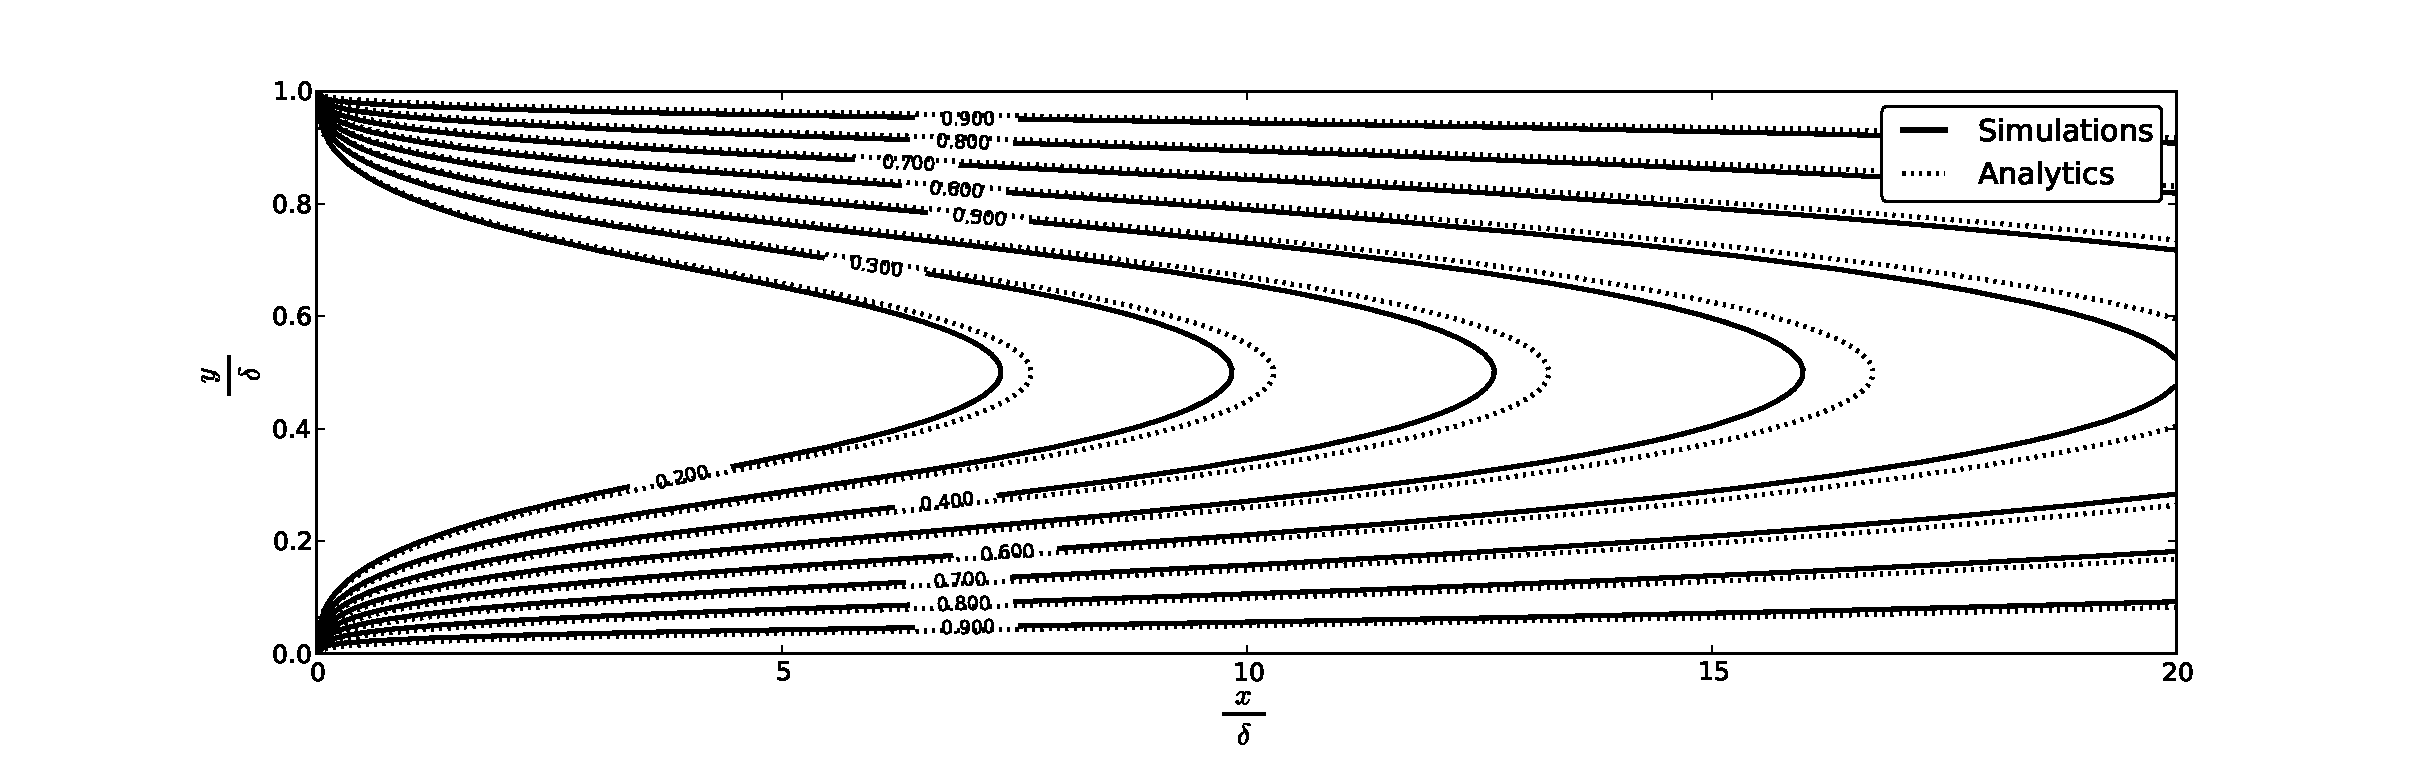
\includegraphics[width=\textwidth]{Figures/parabolic_profile_comparison.eps}
\caption{Comparison between the analytical concentration contours and simulations with pressure
anti bounce-back conditions, Eq. \ref{antibb}. The parameters were
taken as $D=0.0185$ and grid $80\times1600$. \label{fig:parabolic:comparison}}
\end{figure}

After the LBM is validated against the benchmarks relevant for the flow around bubbles, one can
examine all the cases to calculate the volumetric mass transfer coefficient, Section
\ref{section:cases}.

\section{Numerical approach}
\label{sec:numerics}
The multiphase code was utilized to obtain the flow patterns for different capillary numbers
\cite{kuzmin-binary2d}. Five particular cases were chosen to examine, their results are summarized
in Table \ref{table:capillary:cases}. 
\begin{table}[htb!]
\begin{tabularx}{\textwidth}{|X|X|X|X|X|X|X|X|X|}
\hline
$Ca$    &$Re$     &$\ububble$ &$\delta$&$\holdup$
&$\uliq$&$\ugas$&$\lbubble$&$\lslug$\\
\hline
$0.097$ &$1.656$  &$0.0055$ &$0.092$ &$0.30$ &$0.0046$&$0.0016$&$5.79$&$9.21$\\ 
$0.254$ &$4.318$  &$0.0143$ &$0.132$ &$0.28$ &$0.0108$&$0.0041$&$6.12$&$8.88$\\ 
$0.526$ &$8.938$  &$0.0297$ &$0.157$ &$0.27$ &$0.0209$&$0.0080$&$6.19$&$8.81$\\
$0.750$ &$12.744$ &$0.0424$ &$0.167$ &$0.25$ &$0.0293$&$0.0107$&$5.96$&$9.04$\\
$1.040$ &$17.665$ &$0.0588$ &$0.177$ &$0.22$ &$0.0397$&$0.0135$&$5.59$&$9.41$\\
\hline
\end{tabularx}
\caption{Sample results with the binary liquid lattice Boltzmann model \cite{kuzmin-binary2d}. The
following notations are used: the capillary number $Ca=\frac{\ububble L}{\rho \nu}$, $\delta$ is the
non-dimensional film thickness, $\uliq$ is the superficial liquid velocity, $\ugas$ is the
superficial gas velocity. One can see the sketch of the simulation in Fig.
\ref{fig:benchmark:hydro}. \label{table:capillary:cases}}
\end{table}
One can check that velocities in Table \ref{table:capillary:cases} are small. It means that to
match large Peclet numbers, $Pe=\frac{\ububble L}{D}$, usually seen in experiments to measure
the mass transfer coefficient, one needs to decrease
$D=\frac{1}{3}\Bigl(\frac{1}{\omegaminus}-\frac{1}{2}\Bigr)$. However, for parameters
$\omegaminus \approx 0.5$ the stability of the lattice Boltzmann method drastically decreases
\cite{kuzmin-d1q3}. On the other hand, one iteration in the lattice Boltzmann system corresponds
to the time in the physical domain as $\Delta t=U_{\mathrm{bubble,LB}} \frac{\Delta
x}{U_{\mathrm{bubble,phys}}}$. This time is proportional to the velocity of the $U_{\mathrm{LB}}$
and the typical number of simulation steps to obtain necessary number with given velocities for
$Ca<0.2$ is of the order of a few millions. Thus, one wants to increase the available velocity
while keeping the Peclet number the same. This helps to stability of the method as well, since
$\omegaminus$ is not close to its stability limit $\omegaminus=0.5$. 

Given all the considerations above, the approach we take for mass transfer is:
\begin{description}
 \item[Flow field] Given the capillary number $Ca$, one needs to obtain hydrodynamic fields around
the bubble using the binary liquid lattice Boltzmann model according to work
\cite{kuzmin-binary2d}. Periodic boundary conditions are used. The grid used in this work is
$202\times 3000$ which corresponds to fluid domain size $200\times3000$. The grid resolution is
taken to ensure grid
independency of results \cite{kuzmin-binary2d}.  
 \item[Bubble reference frame] Once the hydrodynamics is resolved, the mass transfer simulations
are conducted in the reference frame moving with the bubble. Then the bubble stands still and the
flow is coming around the
bubble. We impose a steady concentration on the surface
of the bubble with the anti bounce-back condition, Eq. \ref{antibb}.
 \item[Velocity improvement] Due to necessity to increase velocity one can scale the velocity to
perform fast simulations, one needs to improve velocity. This issue arises because of the
multiphase model used in simulations. The binary liquid lattice Boltzmann model is the diffusive
interface model. Thus, the
transition between gas and liquid is the continuous function. We obtain the bubble shape according
to the phase indicator $\phi$ as used in \cite{kuzmin-binary2d}, say $\phi<0$. The velocity of the
bubble is calculated as the bubble tip velocity. Because of the highly non-linear diffusive
interface model the shape of the bubble is determined within accuracy of one grid node, as well
there is the error in determination in the bubble velocity. Though these errors are small, however
there is small non-zero velocity component pointing to the bubble in some places, see Fig. 8 in
\cite{kuzmin-binary2d} where some streamlines are penetrating a bubble surface a bit.
This small velocity is amplified upon the velocity scaling and is inconsistent with the
advection-diffusion equation.


Thus, before performing the mass transfer simulations one additional single phase hydrodynamic
simulation is performed. An additional free-surface solver was developed in order to obtain
consistent with the advection-diffusion equation velocity field. We take results from the
multiphase simulations, extract a
bubble shape using the phase indicator $\phi<0$, approximate the bubble shape by the stair-case
line. Then,the obtained bubble velocity is imposed on walls. This corresponds to conducting
simulation in the reference frame moving with the bubble. In addition, the free-slip boundary
condition on the bubble surface is imposed. Appendix \ref{appendix-free-surface} covers the simple
free-slip boundary conditions implementation drastically improving velocity patterns. The system is
iterated until a
steady state is reached. Note, that these type of simulations are much faster than original
multiphase simulations. As the output all the non-zero velocity components perpendicular to the
bubble surface are completely eliminated. We compared original multiphase simulations with
one-component free-slip simulations. All quantities as superficial slug and bubble velocities are
within $3\%$ for the capillary number in the range $0.05\leq Ca \leq 1.0$. This simulation helps to
make mass transfer simulations stable and faster, since the velocity scaling can be done easier and
streamlines are non-penetrating through the interface. One
can see in Fig. \ref{fig:free:surface} two streamlines profiles for $Ca=0.097$  and $Ca=1.040$.
\begin{figure}[htb!]
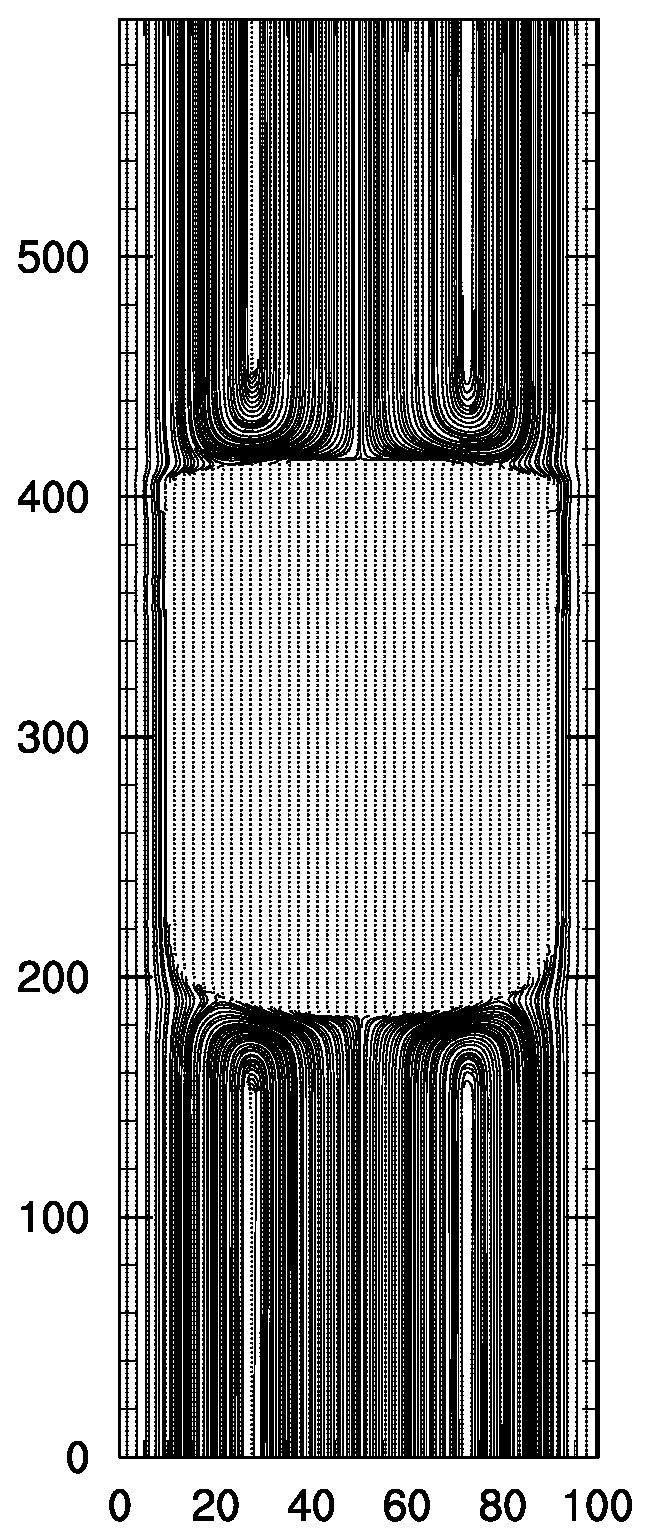
\includegraphics[angle=90,width=\textwidth]{Figures/performed_ca0097.eps}\\
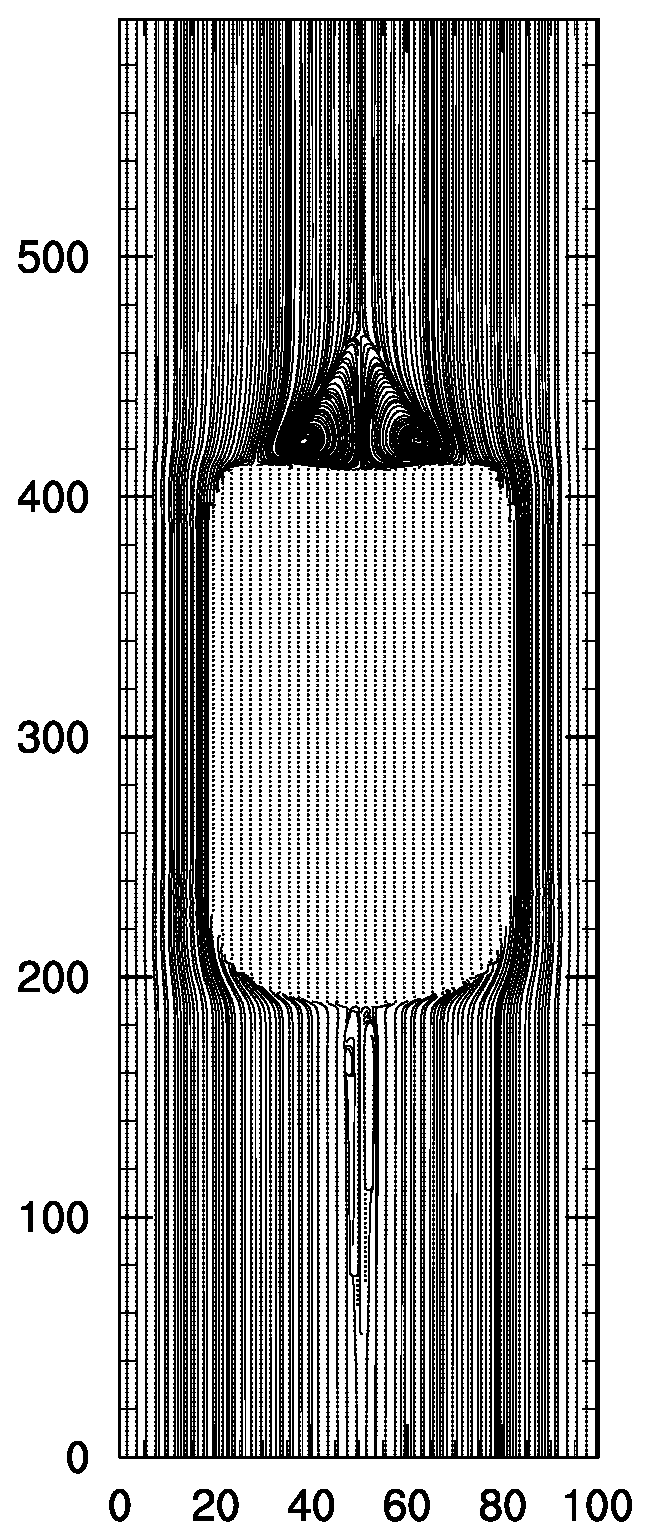
\includegraphics[angle=90,width=\textwidth]{Figures/performed_ca1040.eps}
\caption{The streamlines patterns produced by the free-surface solver with simplistic approximation
of the free-slip bubble surface, see Appendix \ref{appendix-free-surface}. Two completely different
velocity patterns are covered, $Ca=0.097$ (top) and $Ca=1.040$ (bottom).
\label{fig:streamlines:tweaked:velocity}}
\end{figure}

\item[Mass transfer] After improved velocity profiles are obtained one can perform any mass
transfer simulations with different boundary conditions as covered in Section \ref{section:cases}.
For this purpose one needs to match the Peclet number $Pe$ from experiments. Note that we
specifically separated the hydrodynamic problem from the mass transfer problem. When one wants to
solve these simultaneous problems, then one needs to match all the non-dimensional parameters, as
the capillary number (viscous forces over surface tension), the Schmidt number (viscous diffusion
rate over mass diffusion rate), the Peclet number (convection over diffusion), the Reynolds number
(inertia over viscous forces). As the output one can obtain the Sherwood number dependancy on other
parameter (convection mass transfer over diffusion mass transfer):
\begin{equation}
\begin{aligned}
&Re=\frac{\ububble L}{\nu_{\mathrm{liq}}},&&Ca=\frac{\ububble \mu_{\mathrm{liq}}}{\gamma}\\
&Pe=\frac{\ububble L}{D},&&Sh=\frac{K L}{D}\\
&Sc=\frac{\nu_{\mathrm{liq}}}{D}.&&
\end{aligned}
\end{equation}
\end{description}

\section{Results}
This section covers simulation results. We first examine the possibility to increase the fluid
velocity while keeping the Peclet number the same. After that we will examine the periodic boundary
conditions for $5$ capillary number cases,  and finally we will examine
many
cells simulations for two representative cases velocity patterns, as $Ca=0.0907$ and $Ca=1.04$
(see Fig. \ref{fig:streamlines:tweaked:velocity}). 

\subsection{Keeping Peclet}
\label{section:keeping:peclet}
This section addresses the performance of the simulations. The ulimate goal is to increase
velocity at least by several orders of magnitude while keeping dimensionless parameters the same to
speed up                                      
simulations. Increasing velocity can also help to resolve a lot of unit cells to represent a
continous picture.

With the given bubble shape and velocity pattern only nondimensional parameter Peclet number governs
the advection-diffusion equation represented in the lattice Boltzmann system as:
\beq
Pe=\frac{\ububble N_y}{D}.
\feq
As far as we want to increase velocity, that
means one needs to increase the diffusion coefficient as well. The runs were made with
velocities $2,4,6,8,10,15,20,40$ times larger than original velocities. The velocities we chose and
its corresponding capillary numbers are presented in Table \ref{table:scaling:peclet}. Periodic
boundary conditions were used and mass transfer coefficient was calculated according to Eq.
\ref{main:simulation:equation}. Table \ref{table:scaling:peclet} shows that the velocity limit
for  periodic boundary conditions is $0.1$ where $\omegaminus=1.99$ ($D=0.000837$). It gives us the
preliminary idea to what extent one can scale periodic mass transfer simulations. 
\begin{table}[htb!]
\begin{tabularx}{\textwidth}{|X|X|X|X|}
\hline
Scale&$U_{bubble}$&Time Iterations&$C_{aver}$\\
\hline
\multicolumn{4}{c}{}\\
\multicolumn{4}{c}{$Ca=0.097$,$Pe=1313$}\\
\hline
$2$ &$0.011$&$400000$&$0.318$\\
$4$ &$0.023$&$200000$&$0.319$\\
$8$ &$0.044$&$100000$&$0.320$\\
$10$&$0.055$&$80000$ &$0.321$\\
$20$&$0.11 $&$40000$ &$0.324$\\
$40$&$0.22 $&$20000$ &$0.328$\\
\hline
\multicolumn{4}{c}{}\\
\multicolumn{4}{c}{$Ca=0.254$,$Pe=3414$}\\
\hline
$2$& $0.0286$&$800000$&$0.6533$\\
$4$& $0.0572$&$400000$&$0.6591$\\
$8$& $0.1144$&$200000$&$0.6692$\\
$10$&$0.1430$&$160000$&$0.6734$\\
$20$&$0.2860$&$80000$ &$0.6894$\\
\hline
\multicolumn{4}{c}{}\\
\multicolumn{4}{c}{$Ca=0.526$,$Pe=7092$}\\
\hline
$2$&$0.0594$&$200000$&$0.3271$\\
$4$&$0.1188$&$100000$&$0.3315$\\
\hline
\multicolumn{4}{c}{}\\
\multicolumn{4}{c}{$Ca=0.750$,$Pe=10125$}\\
\hline
$2$&$0.0848$&$200000$&$0.3489$\\
\hline
\multicolumn{4}{c}{}\\
\multicolumn{4}{c}{$Ca=1.040$,$Pe=14041$}\\
\hline
$2$&$0.1176$&$200000$&$0.3675$\\
\hline
\end{tabularx}
\caption{This table presents the achievable stable velocity $\ububble$ when one scales velocity. One
iteration in the lattice
Boltzmann system corresponds to time difference as
$\Delta t=\frac{U_{\mathrm{bubble,LB}}}{U_{\mathrm{bubble,phys}}} \Delta x$. Therefore the speed up
of the simulation is proportional to the  $U_{\mathrm{bubble,LB}}$. Note that all time
iterations
indicated in the table correspond to the one time moment in physical space. One can see that
scaling produces adequate results.  The achievable stable velocity is around $U_{bubble}=0.1$ for
the diffusion coefficient
$D=1/3(1/1.99-0.5)=0.000837$. Average concentrations are in the reasonable agreement. The contour
profiles for all of these cases (capillary number $Ca$ and all scales) are presented in Fig.
\ref{fig:contours:scaling:peclet}.
\label{table:scaling:peclet}}
\end{table}
The corresponding to Table \ref{table:scaling:peclet} concentration contour profiles for different
velocity scalings are presented in Fig. \ref{fig:contours:scaling:peclet}. One can see an
acceptable agreement between all of them. Note, that a few profiles are obtained $10$ to $40$ times
faster.
\begin{figure}[htb!]
\includegraphics[height=0.25\textwidth]{Figures/contourlines_scale_ca097.eps}\\
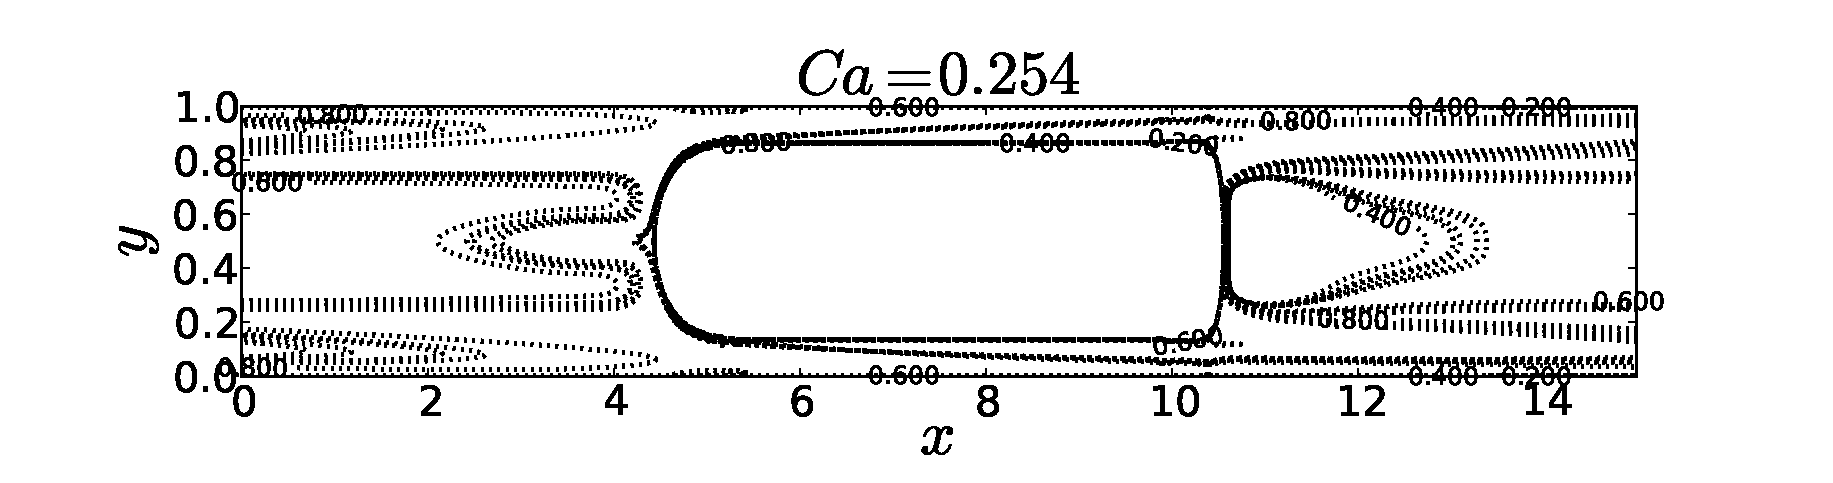
\includegraphics[height=0.25\textwidth]{Figures/contourlines_scale_ca054.eps}\\
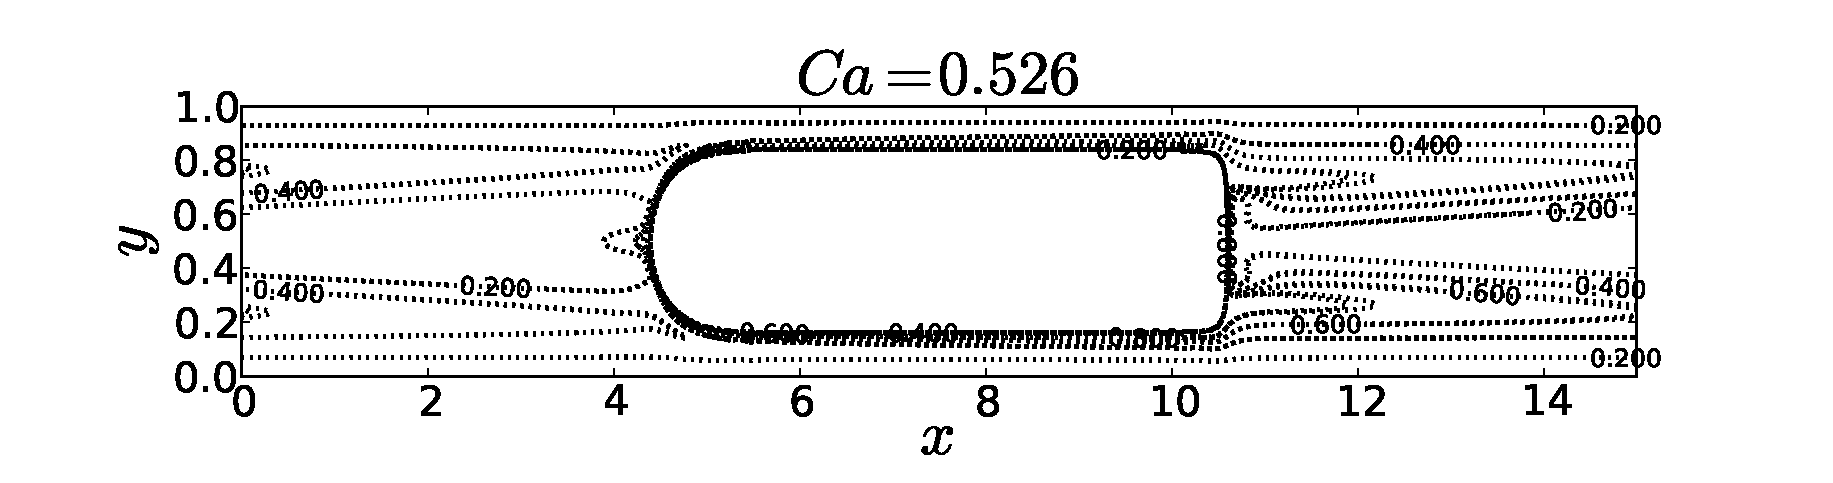
\includegraphics[height=0.25\textwidth]{Figures/contourlines_scale_ca026.eps}\\
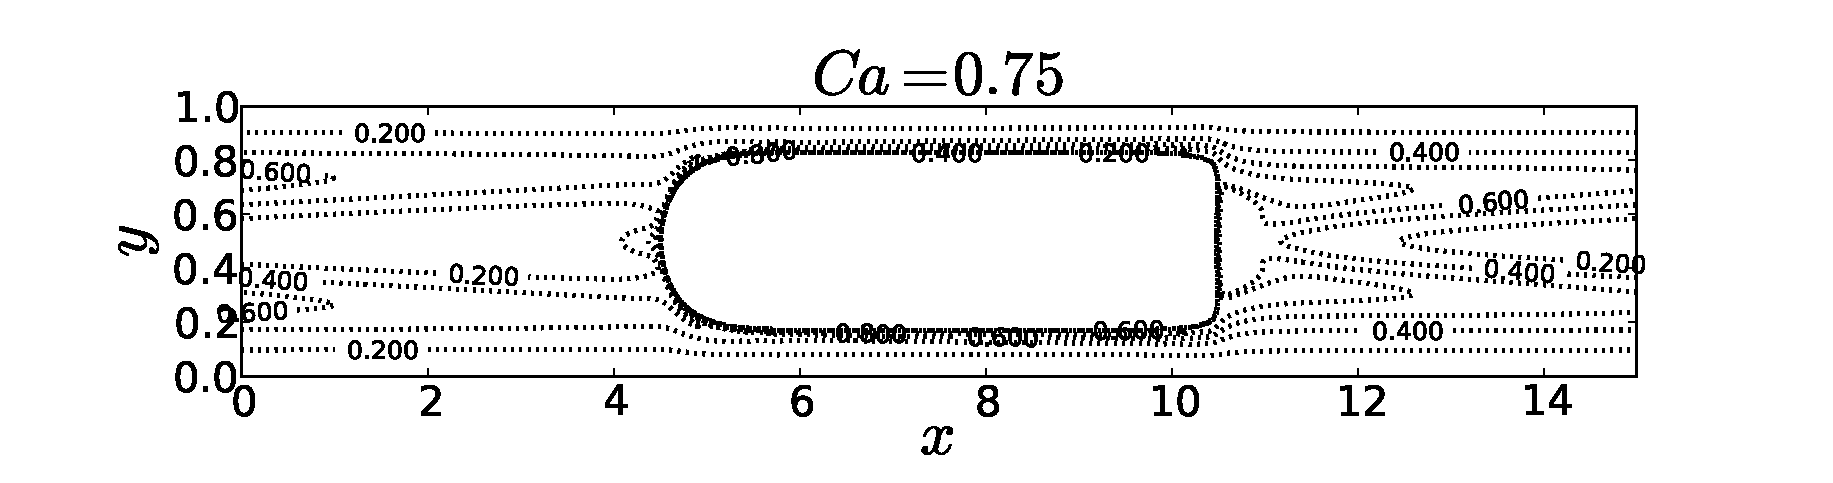
\includegraphics[height=0.25\textwidth]{Figures/contourlines_scale_ca05.eps}\\
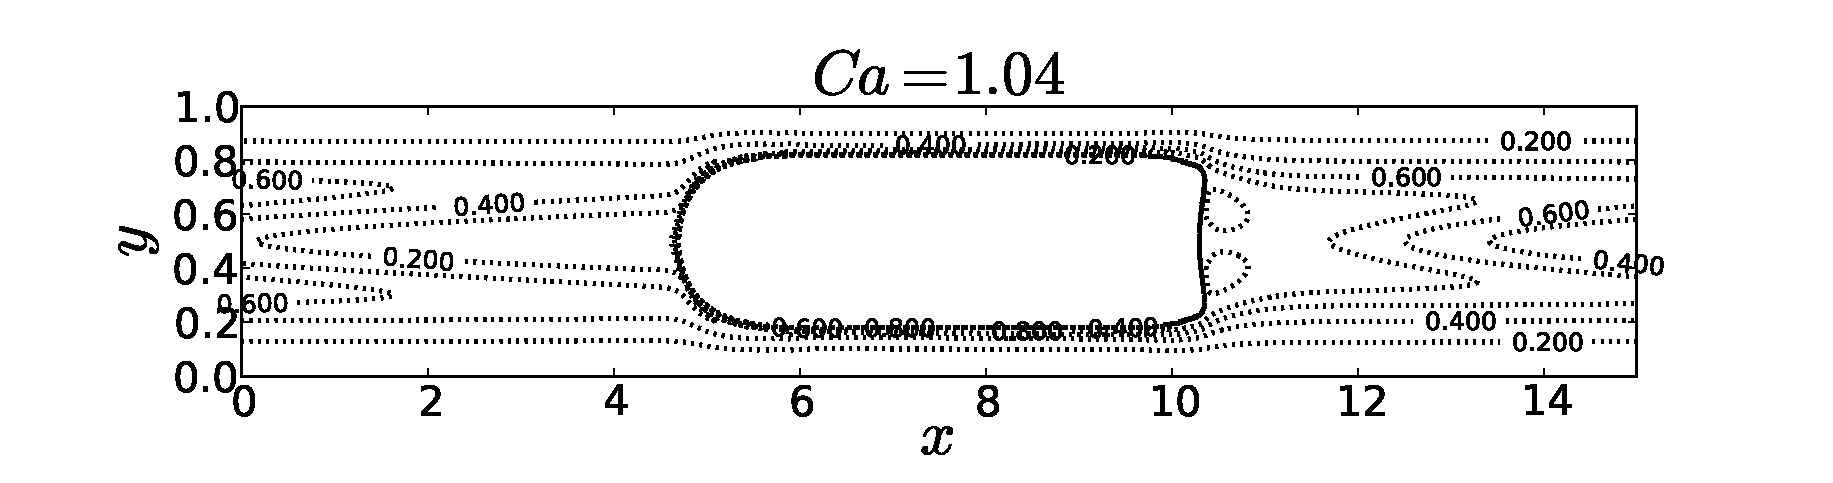
\includegraphics[height=0.25\textwidth]{Figures/contourlines_scale_ca14.eps}\\
\caption{Concentration contour profiles for velocity scalings as identified in Table
\ref{table:scaling:peclet} (top to bottom:
$Ca=0.097,0.254,0.526,0.750,1.040$). Thick lines correspond to
all different scales indicated in Table
\ref{table:scaling:peclet}. Agreement is reasonable. \label{fig:contours:scaling:peclet}}
\end{figure}

\subsection{Average concentration}
\label{main:results:periodic}
As indicated in Section \ref{section:cases} one can calculate the average domain concentration over
the time. Eq. \ref{theor:one:concentration:time} shows how 
the volumetric mass transfer coefficient depends on
time, i.e. streamwise coordinate:
\beqal
&\vol t \frac{\ububble}{\ugas+\uliq}=\ln\frac{\cstar}{\cstar-\langle C(t) \rangle}\\
&\vol \frac{\lunit}{\ugas+\uliq}=\frac{\lunit}{\ububble t} \ln \frac{C^*}{C^*-\langle C(t)
\rangle},\\
\feqal
where $\langle C(t) \rangle$ is the average concentration in the whole liquid domain.
Simulations for coefficient $\vol \frac{\ububble}{\ugas+\uliq}$ are shown in Fig.
\ref{fig:aver:conc:different:capillaries:time} for different Peclet numbers and velocity scalings
indicated in Table \ref{table:scaling:peclet}. Because in the definition of the volumetric mass
transfer coefficient there is the logarithm function, thus when the average concentration goes
close to $\cstar=1$ then Eq. \ref{theor:one:concentration:time} gives inadequate results due to
 accuracy of the logarithmic function. Fig. \ref{fig:aver:conc:different:capillaries:time} presents
the volumetric mass transfer coefficient against number of time iterations. However, due to scaling
each simulation has a different physical time step. We scaled curves against number of cell
units which tracer will pass with the given bubble velocity, i.e. 
$N_{\text{cell\,units}}=\frac{\text{scale} \ububble t}{\lunit}$.  Fig.
\ref{fig:aver:conc:different:capillaries} shows the volumetric mass transfer
dependency against the distance in unit cells length. One can see in Table
\ref{table:steady:state:average} that for different Peclet numbers different time (number of unit
cells) is required to achieve the steady state. For example, for
larger Peclet number less time steps are required to achieve the steady state condition. 

Overall one is guaranteed to obtain the steady state volumetric mass transfer coefficient for
periodic boundaries simulations if the following conditions are fulfilled:
\begin{description}
\item[I] Scaling is performed as $U_{max}=\mathrm{scale}\cdot\ububble\leq 0.1$.
\item[II] The larger Peclet number the less time is required. One can extrapolate data from Table
\ref{table:steady:state:average}, say $L_{\mathrm{steady}}$ and perform the following number of
iterations as $\mathrm{scale}\cdot \ububble\cdot N_{\mathrm{iter}}\leq L_{\mathrm{steady}}$. 
\end{description}
Also, Table \ref{table:steady:state:average} shows
the achieved steady state volumetric mass transfer coefficient. 
\begin{figure}[htb!]
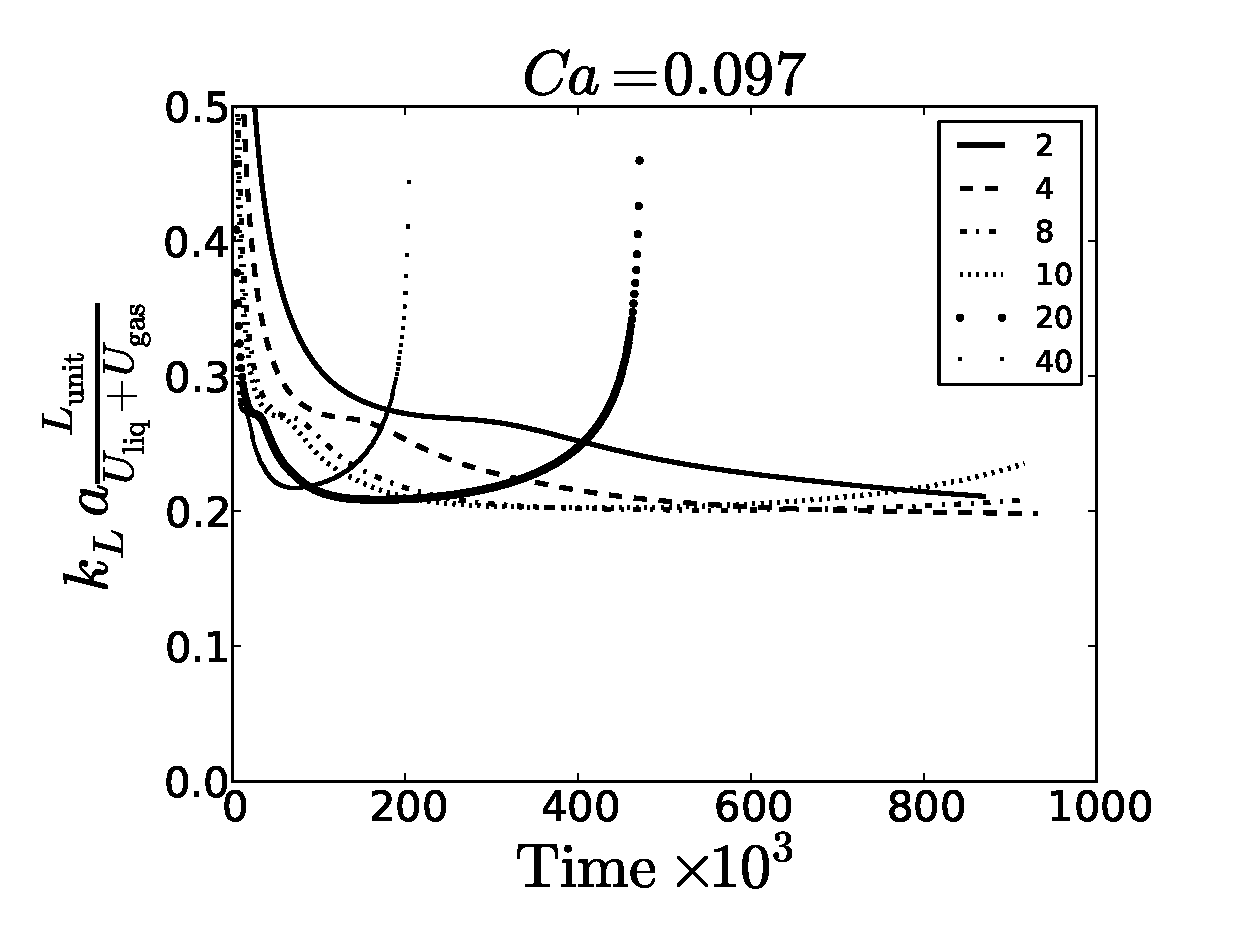
\includegraphics[width=0.5\textwidth]{Figures/aver_conc_scale_ca_time097.eps}
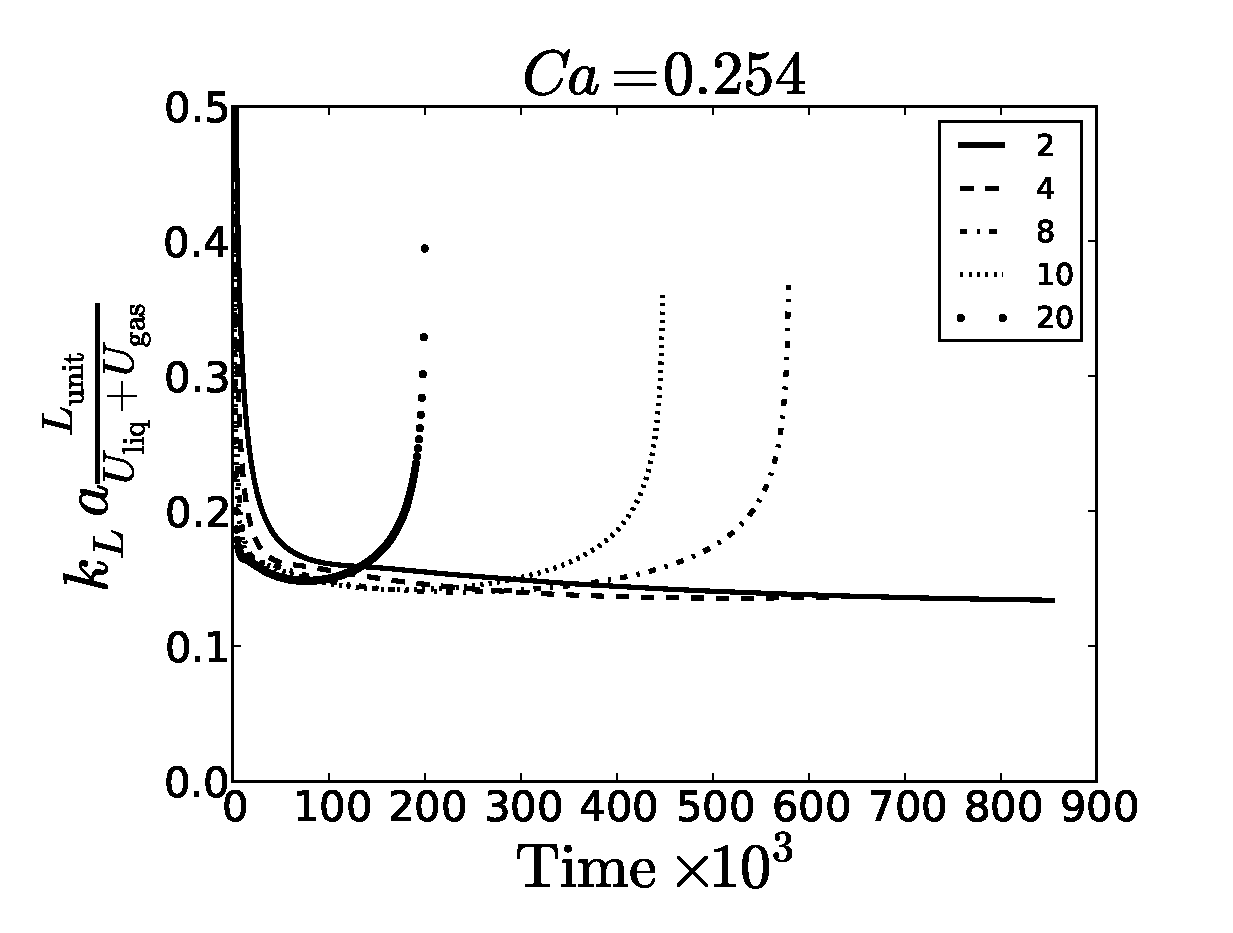
\includegraphics[width=0.5\textwidth]{Figures/aver_conc_scale_ca_time054.eps}\\
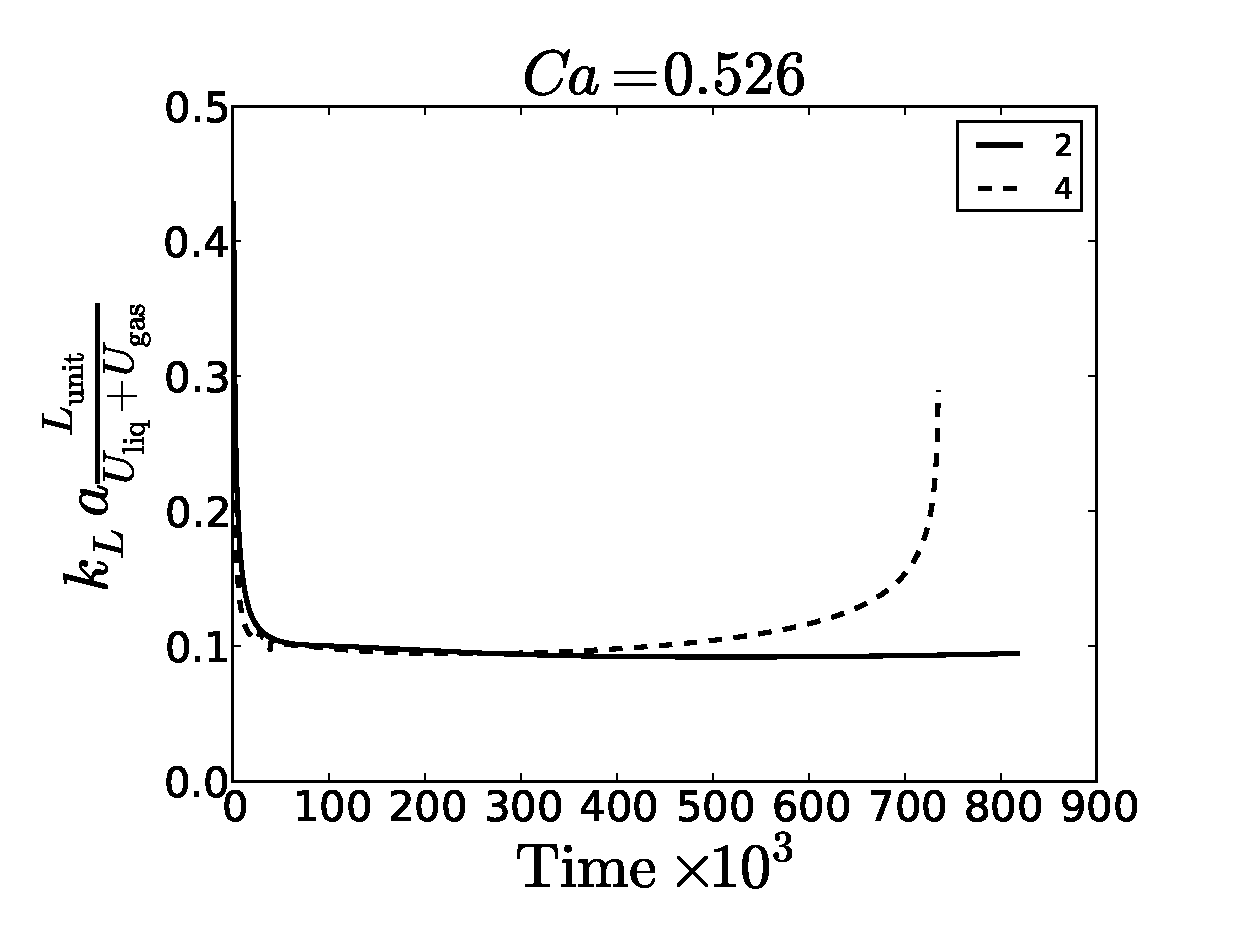
\includegraphics[width=0.5\textwidth]{Figures/aver_conc_scale_ca_time026.eps}
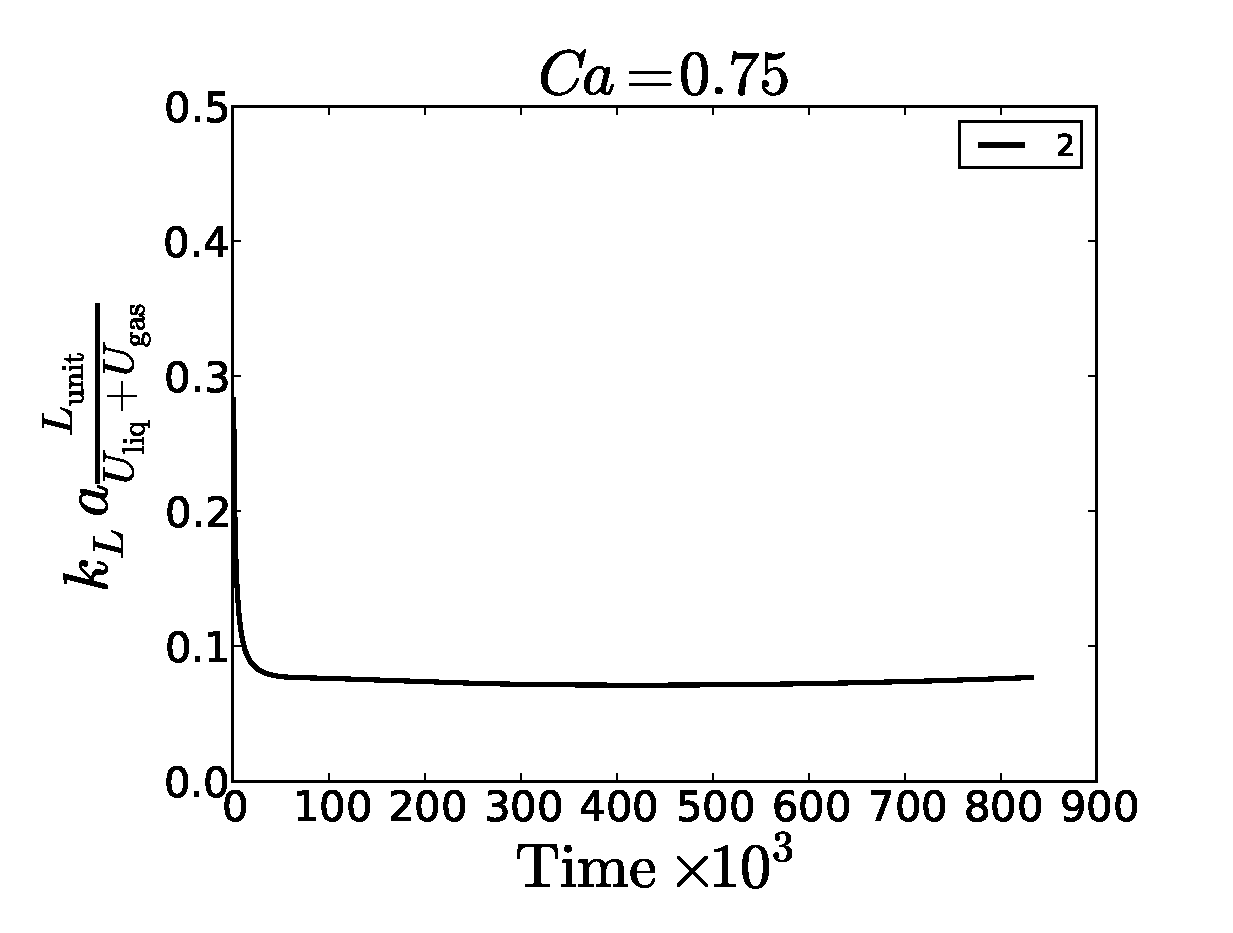
\includegraphics[width=0.5\textwidth]{Figures/aver_conc_scale_ca_time05.eps}\\
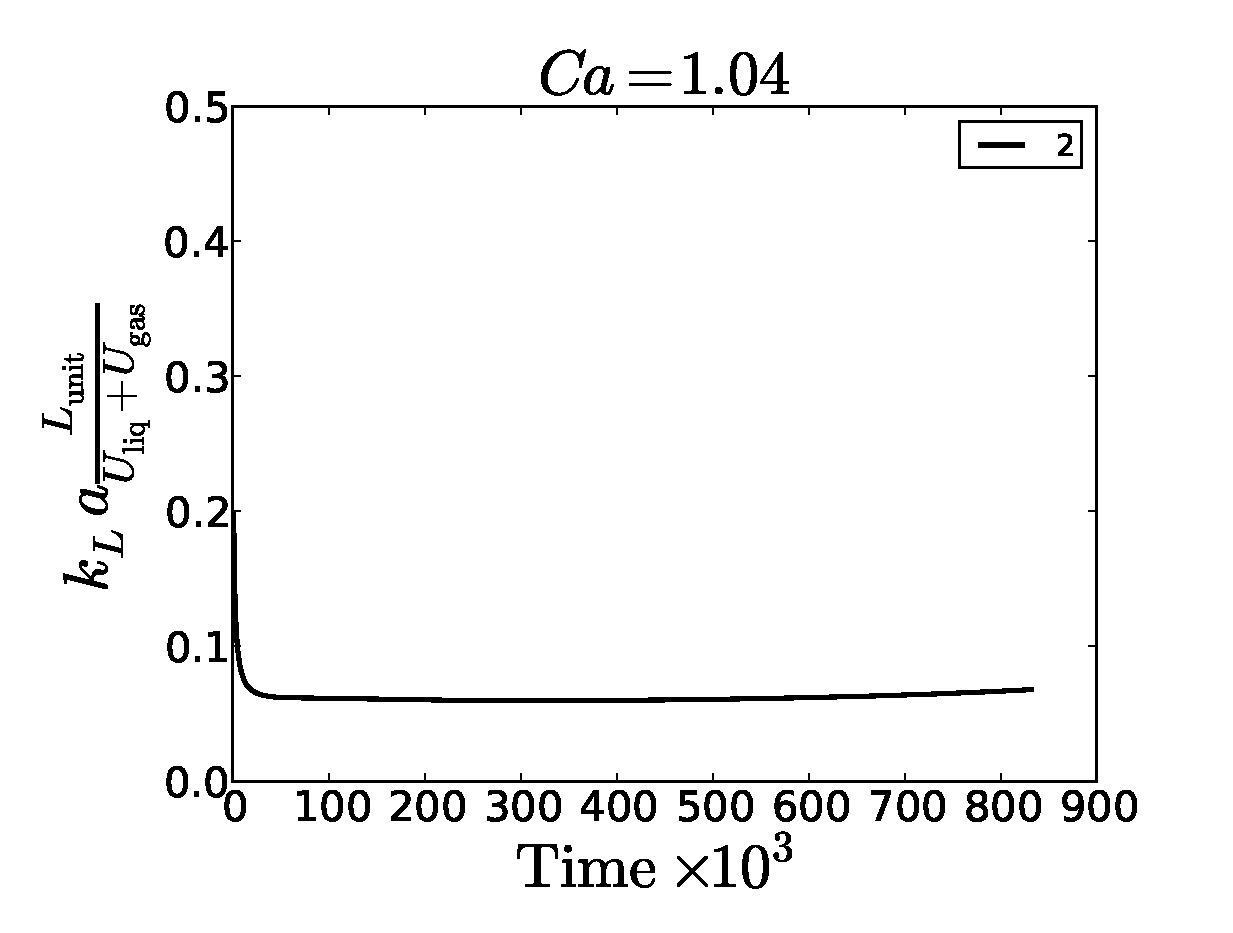
\includegraphics[width=0.5\textwidth]{Figures/aver_conc_scale_ca_time14.eps}
\caption{Calculated volumetric mass transfer coefficient for different capillaries and scales
against time. One can see
that all curves have the same minimum corresponding to the volumetric mass transfer coefficient.
Some simulations show the volumetric mass transfer coefficient going up due to the average
concentration being close to $\cstar$. All of them show an excellent agreement. Note, that with the
scaling one can reduce the amount of calculations drastically. However, one needs to be attentive
because with the large velocity scaling average concentration can quickly approach $\cstar$, thus
getting an infinite volumetric mass transfer coefficient.
\label{fig:aver:conc:different:capillaries:time}}
\end{figure}
\begin{figure}[htb!]
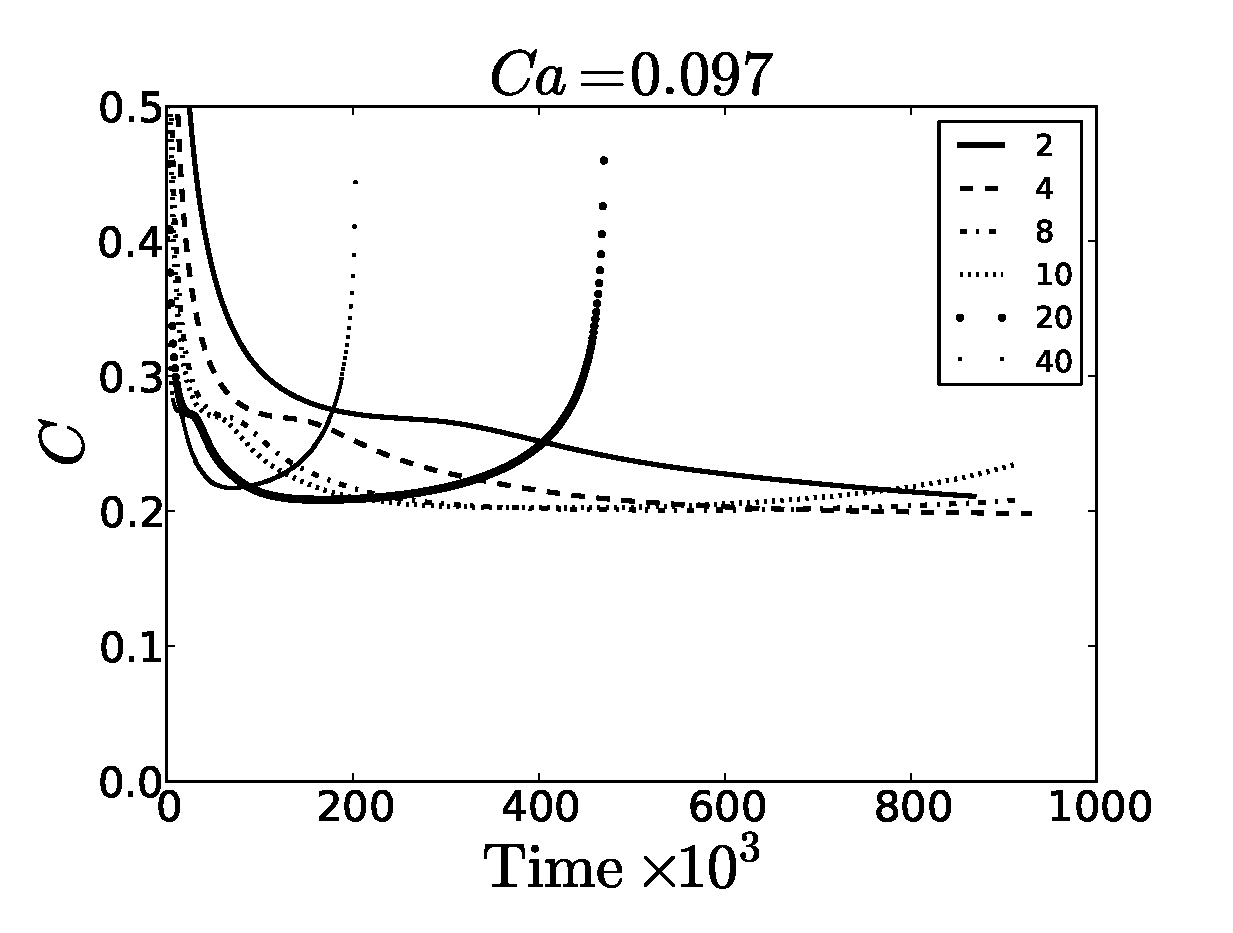
\includegraphics[width=0.5\textwidth]{Figures/aver_conc_scale_ca097.eps}
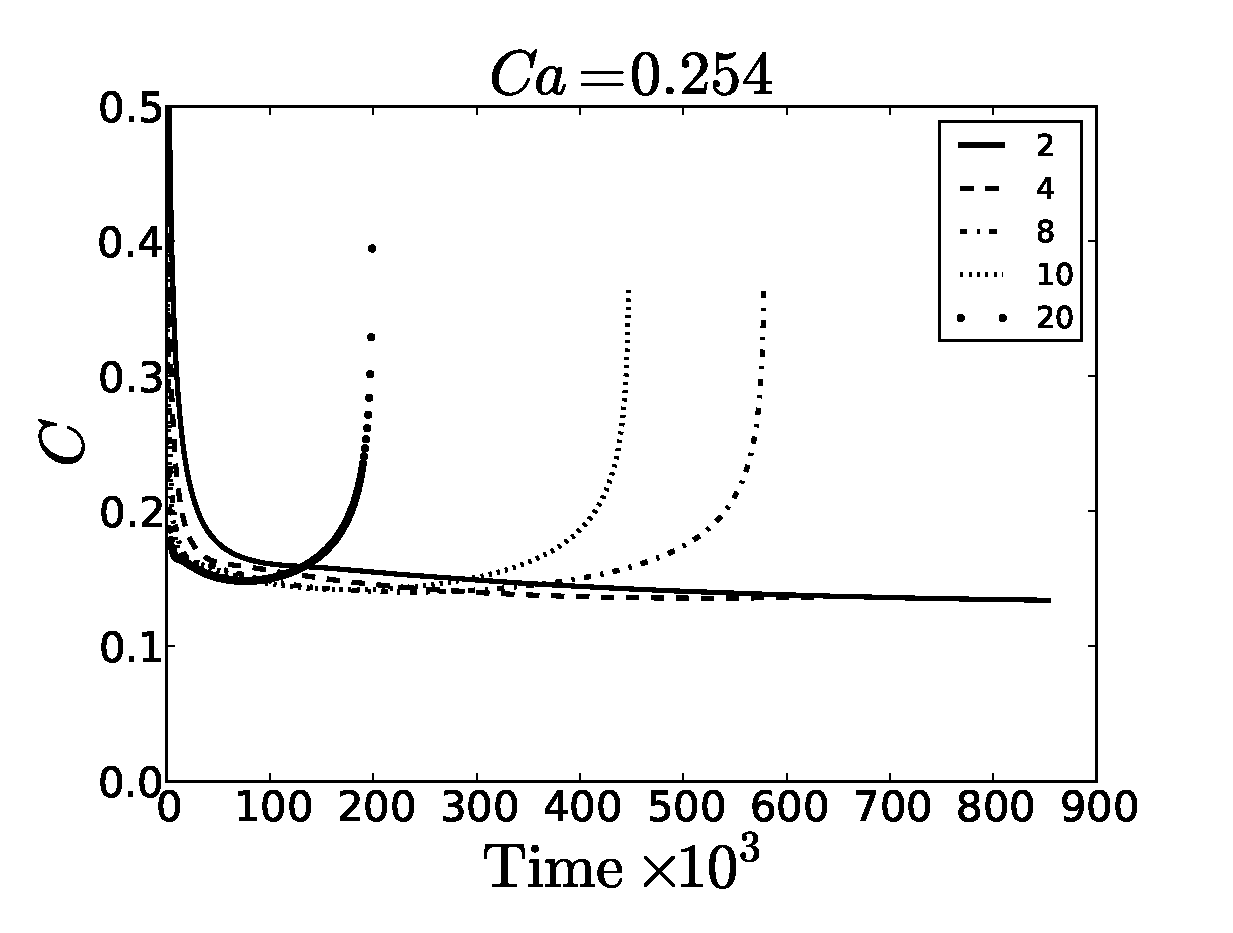
\includegraphics[width=0.5\textwidth]{Figures/aver_conc_scale_ca054.eps}\\
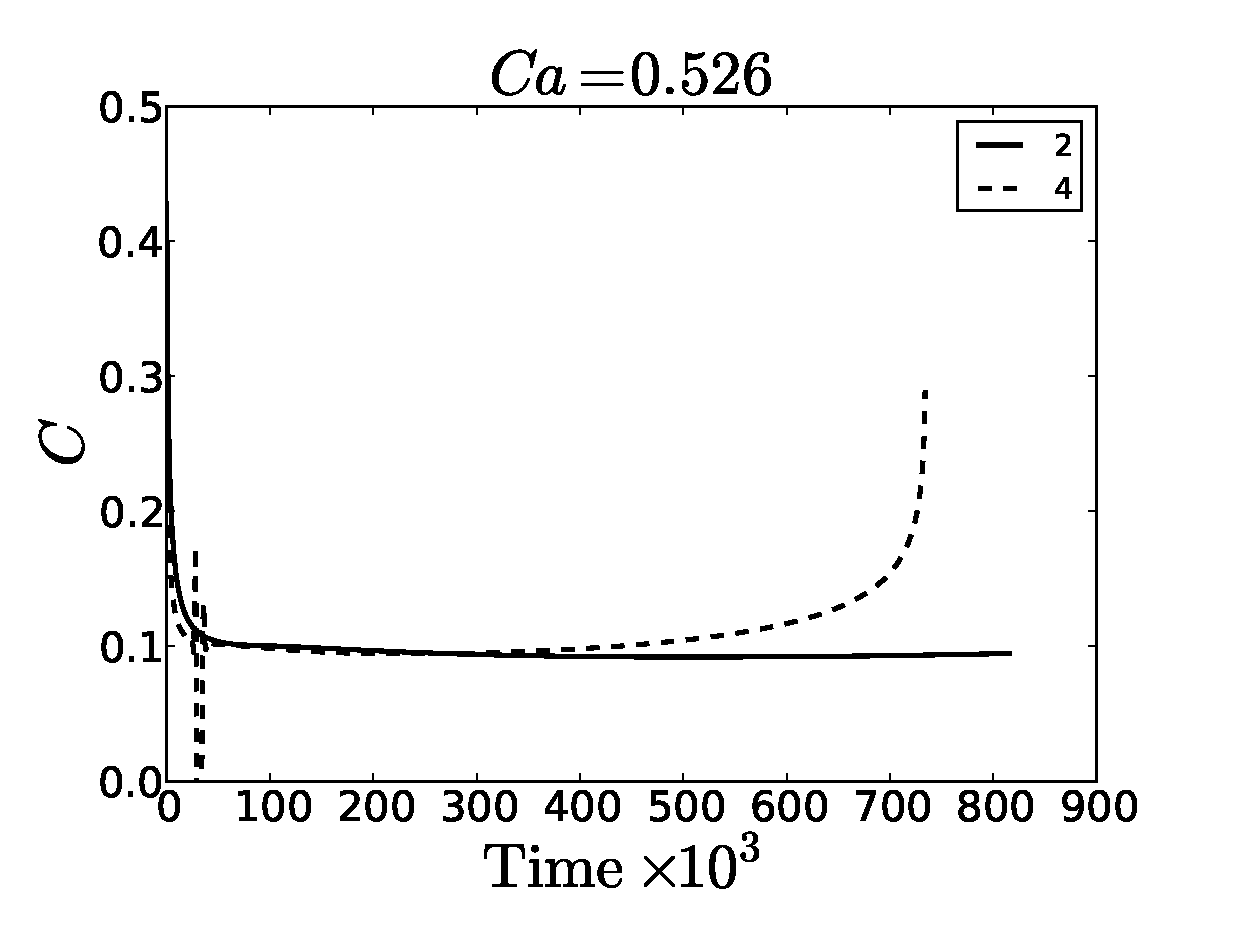
\includegraphics[width=0.5\textwidth]{Figures/aver_conc_scale_ca026.eps}
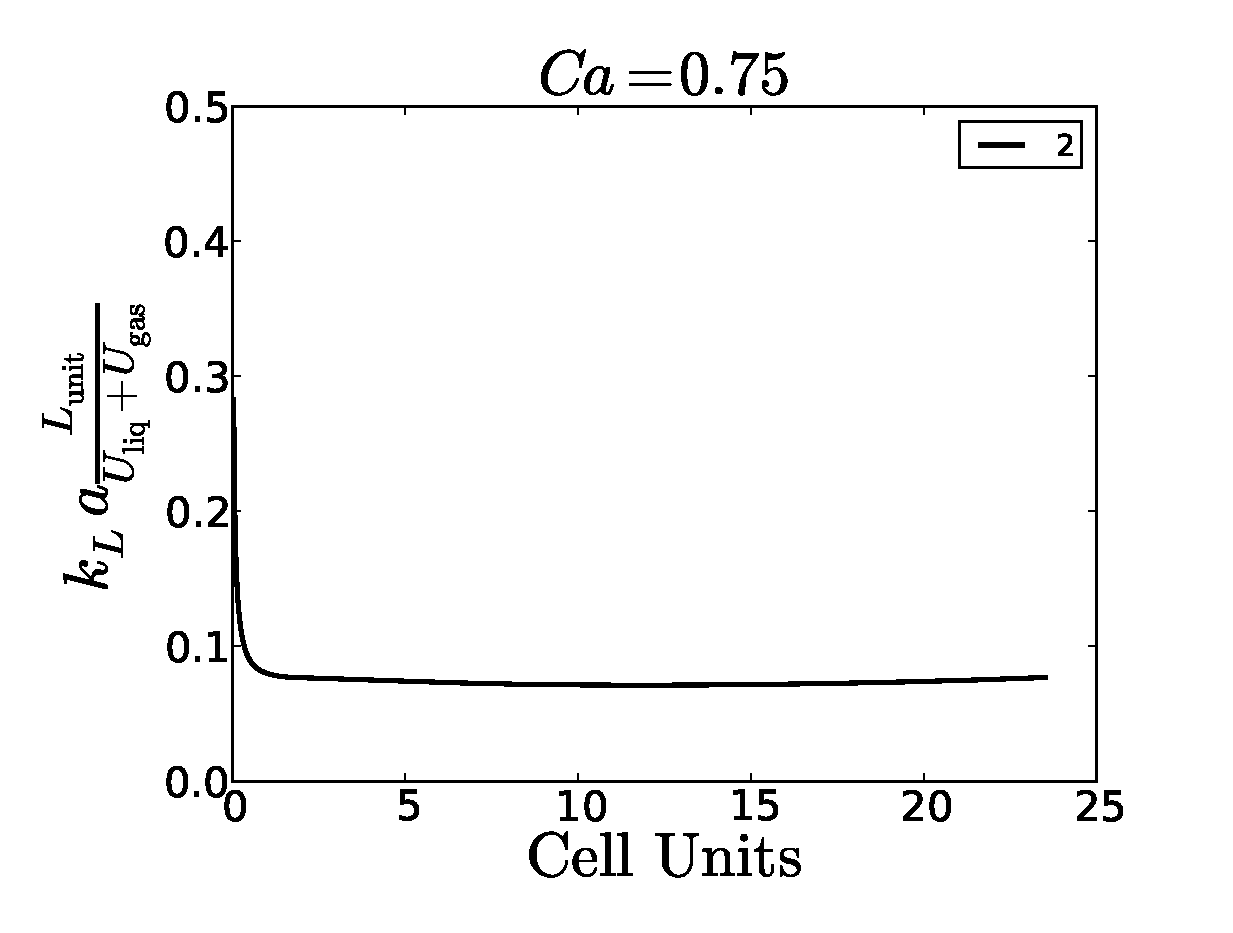
\includegraphics[width=0.5\textwidth]{Figures/aver_conc_scale_ca05.eps}\\
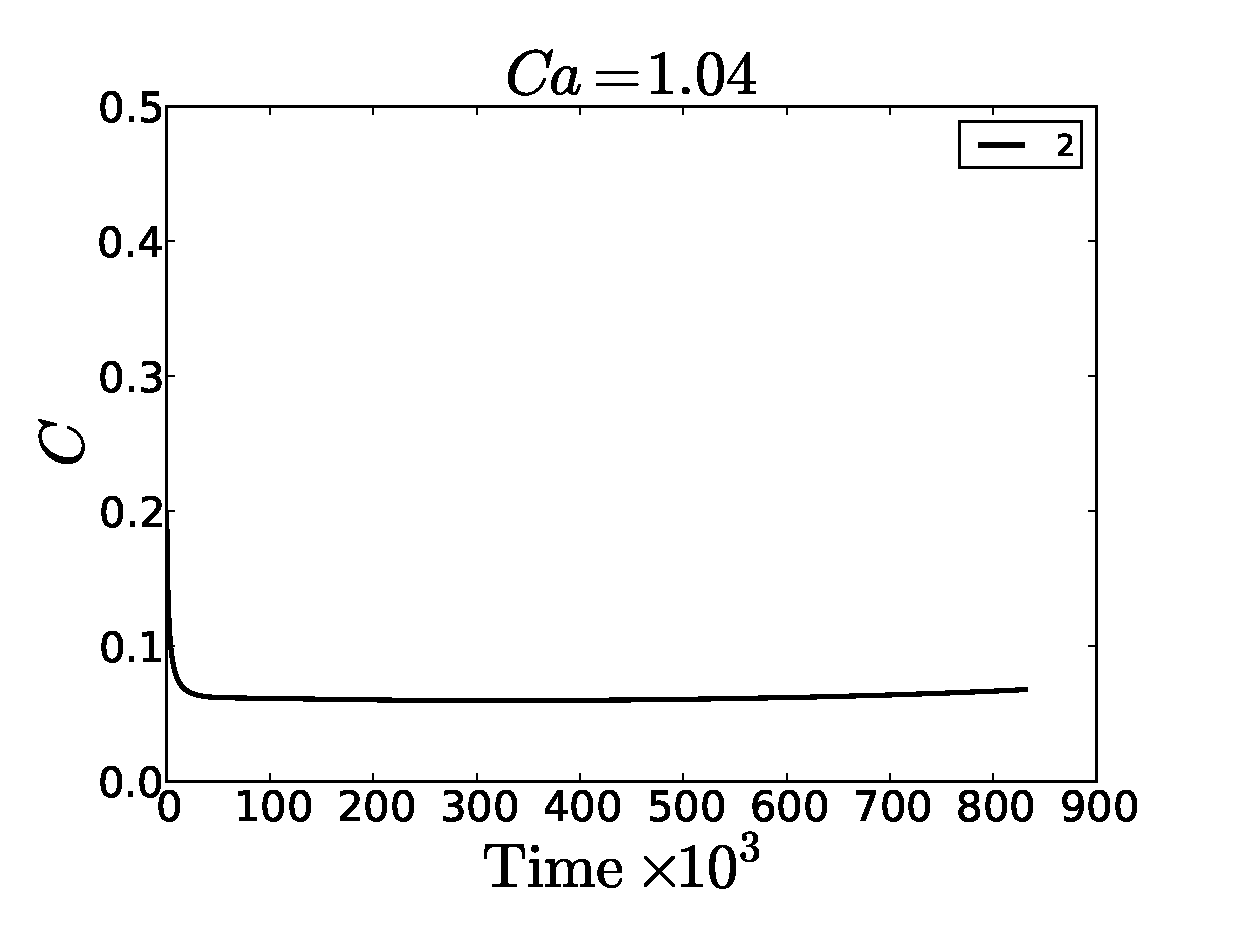
\includegraphics[width=0.5\textwidth]{Figures/aver_conc_scale_ca14.eps}
\caption{Volumetric mass transfer coefficient for different capillaries and scales against the
bubble traveling distance in the laboratory frame. ''Cell Units`` axis is refered to the physical
distance of how many unit cells the bubble passes until the steady state is reached. Table
\ref{table:steady:state:average}
summarizes results.\label{fig:aver:conc:different:capillaries}}
\end{figure}
\begin{table}[htb!]
\begin{tabularx}{\textwidth}{|X|X|X|X|}
\hline
$Ca$    &$Pe$     &$L_{\mathrm{steady}}/\lunit$& $\volnondim$ \\
\hline
$0.097$ &$1313$  &$7$&$0.21$  \\ 
$0.254$ &$3414$  &$6$&$0.14$  \\ 
$0.526$ &$7092$  &$3$&$0.095$ \\
$0.750$ &$10125$ &$3$&$0.074$ \\
$1.040$ &$14041$ &$2$&$0.0601$\\
\hline
\end{tabularx}
\caption{The distance which a bubble propagates when the
steady-state condition is achieved. One can see that increasing
Peclet number helps to achieve the steady state faster.\label{table:steady:state:average}}
\end{table}

\subsection{Periodic boundaries with the inlet/outlet characteristic concentration}
\label{results:periodic:inlet:outlet}
When the characteristic concentration is taken as in the formulation of \citet{vanbaten-circular},
i.e. the inlet/outlet flux averaged concentration, then the results are quite different. One can
see in Fig. \ref{fig:volumetric:char:concentration:vanbaten} the calculated volumetric mass transfer
is different from the domain averaged calculated volumetric mass transfer coefficient. For example,
for small capillary numbers, i.e. $Ca=0.097,0.254,0.526$ the predicted values are overpredicted
($\volnondim=0.3,0.25,0.1$). When the velocity pattern is changed from having vortex in front of
the bubble to not having it,  i.e. $Ca=0.75,1.04$ the calculated values
are underpredicted than in the previous case, i.e. $\volnondim=0.06,0.04$.
\begin{figure}[htb!]
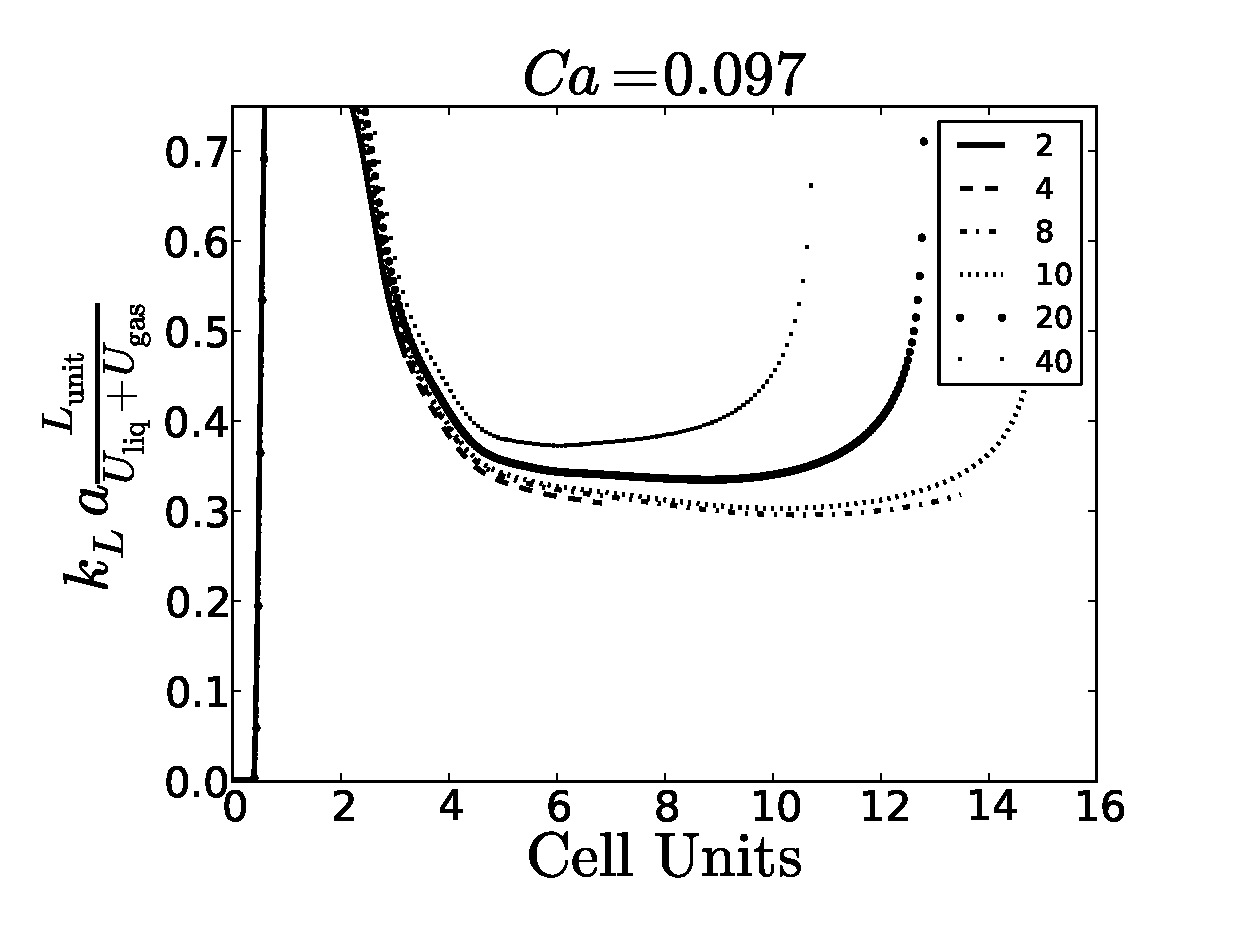
\includegraphics[width=0.5\textwidth]{Figures/aver_vanbaten_scale_ca097.eps}
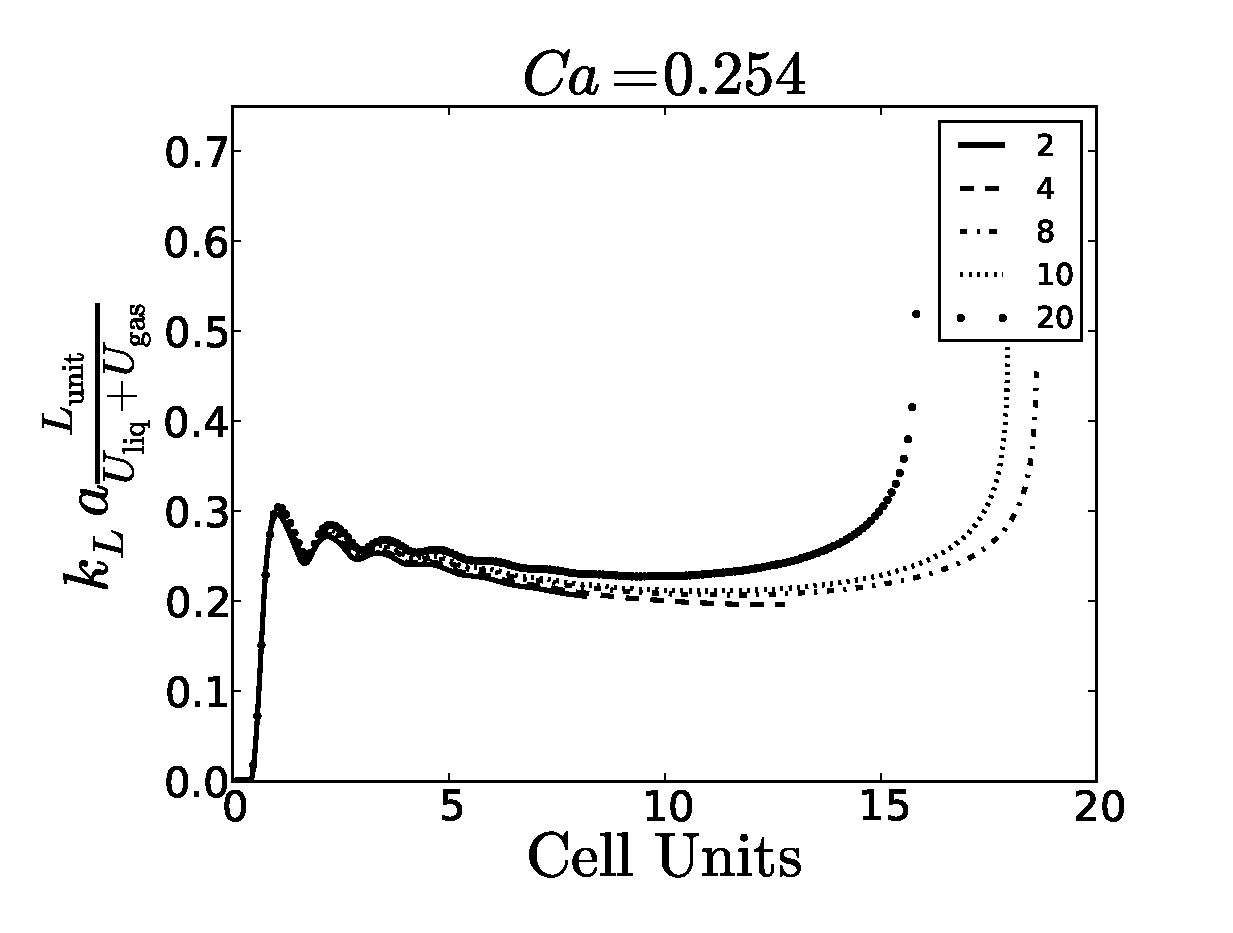
\includegraphics[width=0.5\textwidth]{Figures/aver_vanbaten_scale_ca054.eps}\\
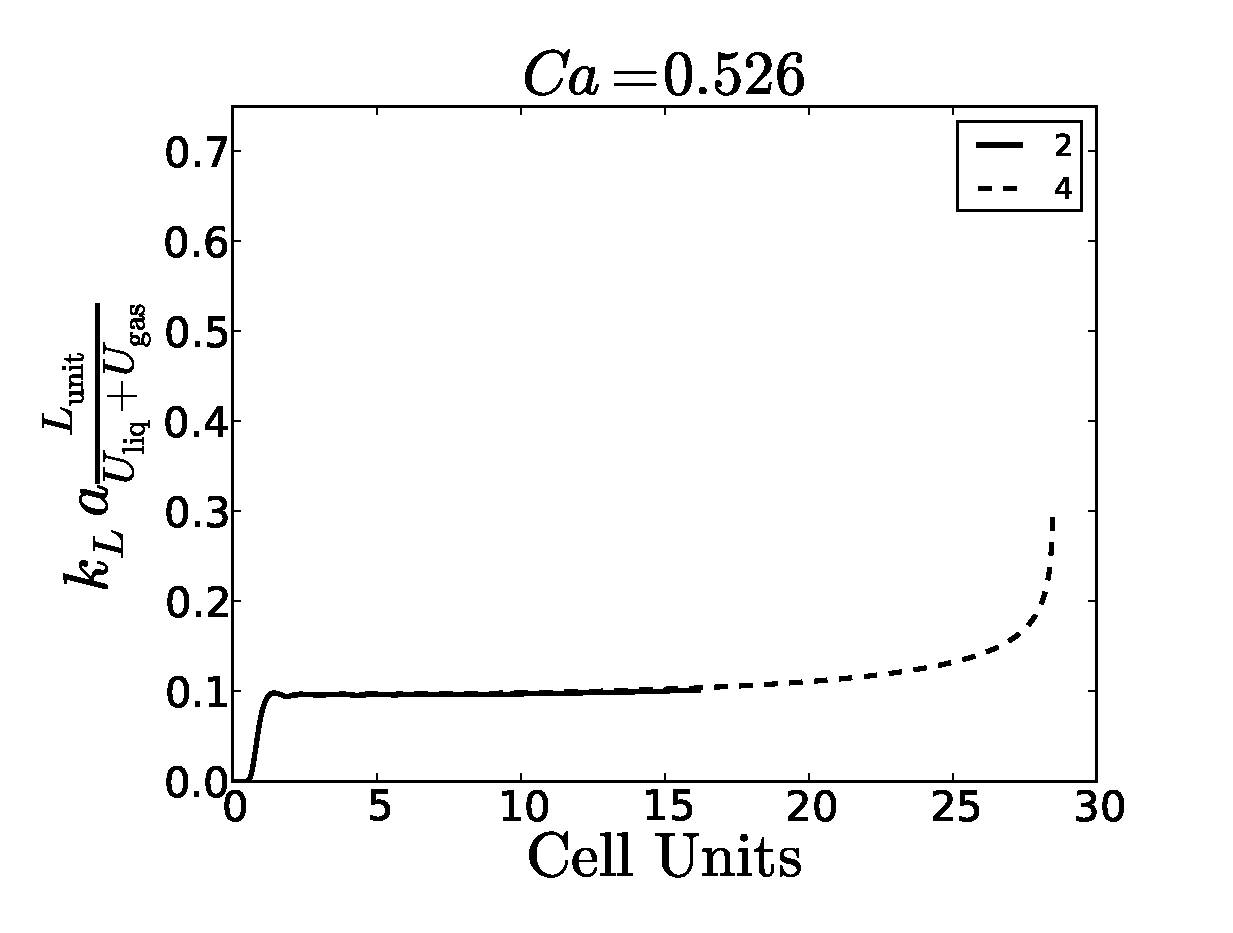
\includegraphics[width=0.5\textwidth]{Figures/aver_vanbaten_scale_ca026.eps}
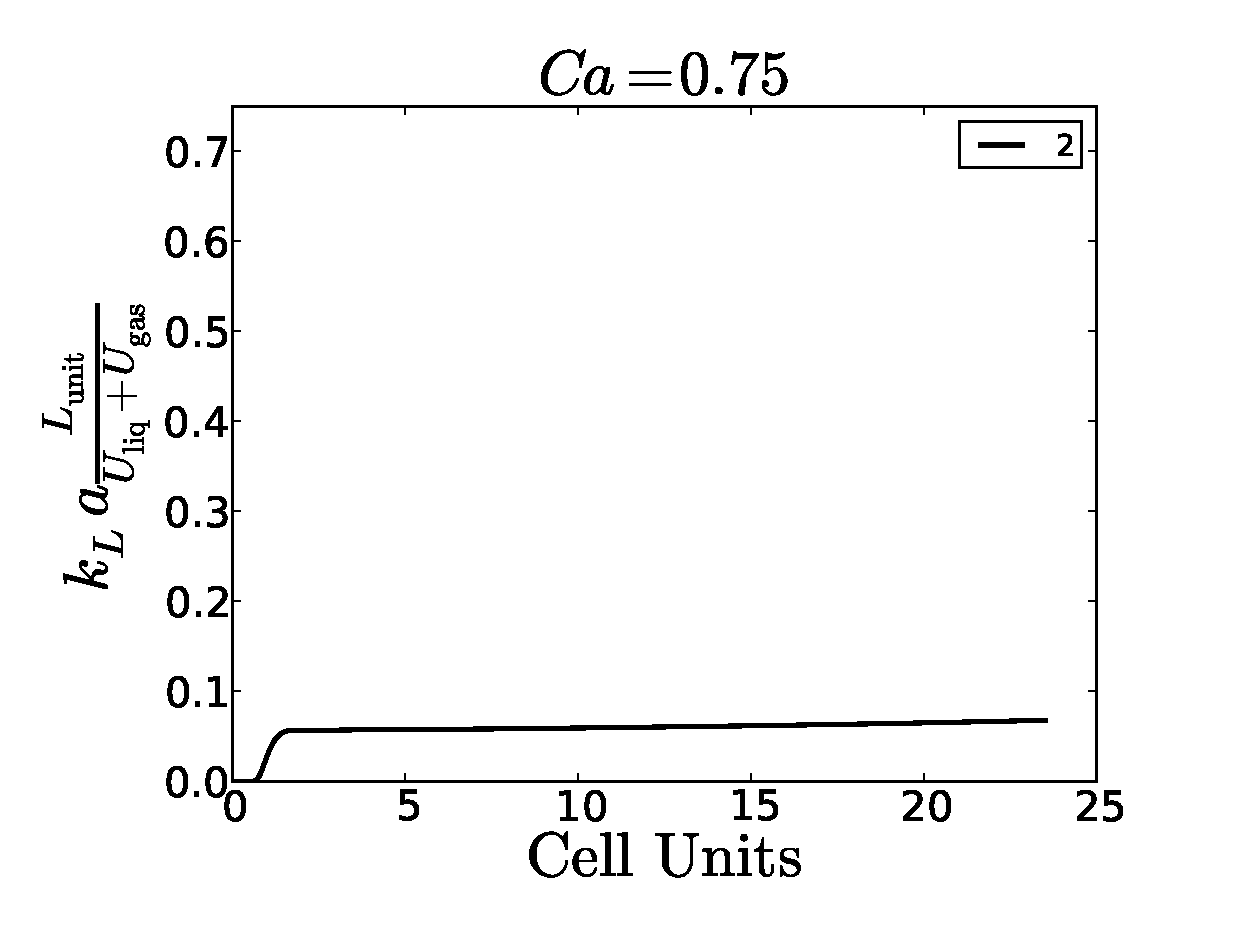
\includegraphics[width=0.5\textwidth]{Figures/aver_vanbaten_scale_ca05.eps}\\
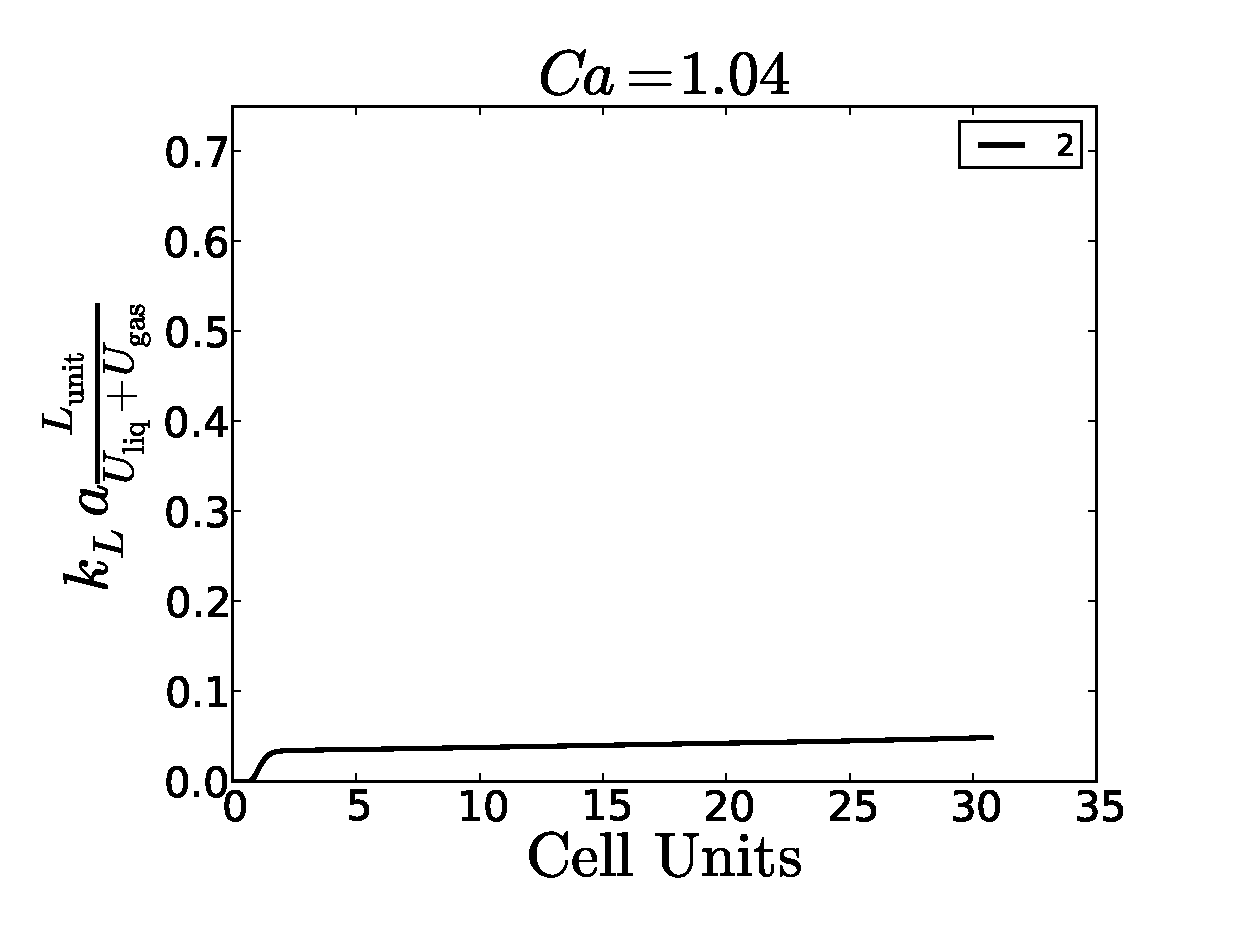
\includegraphics[width=0.5\textwidth]{Figures/aver_vanbaten_scale_ca14.eps}
\caption{The volumetric mass transfer coefficient
with the characteristic concentration based on
the inlet/outlet flux averaged concentration as
in \cite{vanbaten-circular}. One can see that values are either overpredicted or underpredicted
than values specified in Table \ref{table:steady:state:average} depending on the velocity pattern. 
\label{fig:volumetric:char:concentration:vanbaten}}
\end{figure}


\subsection{\citeauthor{vanbaten-circular} formulation}
\label{results:vanbaten}
The van Baten formulation which is calculated as the change of mass in domain with characteristic
concentrations to be as the average domain simulation and as the averaged flux input/output
concentration. One can see them in Fig. \ref{fig:vanbaten} for $Ca=0.097$ and
$Ca=1.04$. One can see that results are consistent with the simulations in Section
\ref{main:results:periodic} for the volumetric mass transfer coefficient measured with the domain
averaged concentration in the whole range of capillary numbers. Note that for $Ca=0.097$ the
obtained mass transfer coefficient is less than in Section \ref{main:results:periodic}. However, as
it will be shown later the obtained volumetric mass transfer coefficient for $Ca=0.0097$ has the
same value as for the simulations of a few unit cells. The
inlet/outlet
flux averaged concentration is shown to be consistent only for velocity patterns related to larger
Capillary numbers, i.e. $Ca\geq0.7$. 
\begin{figure}
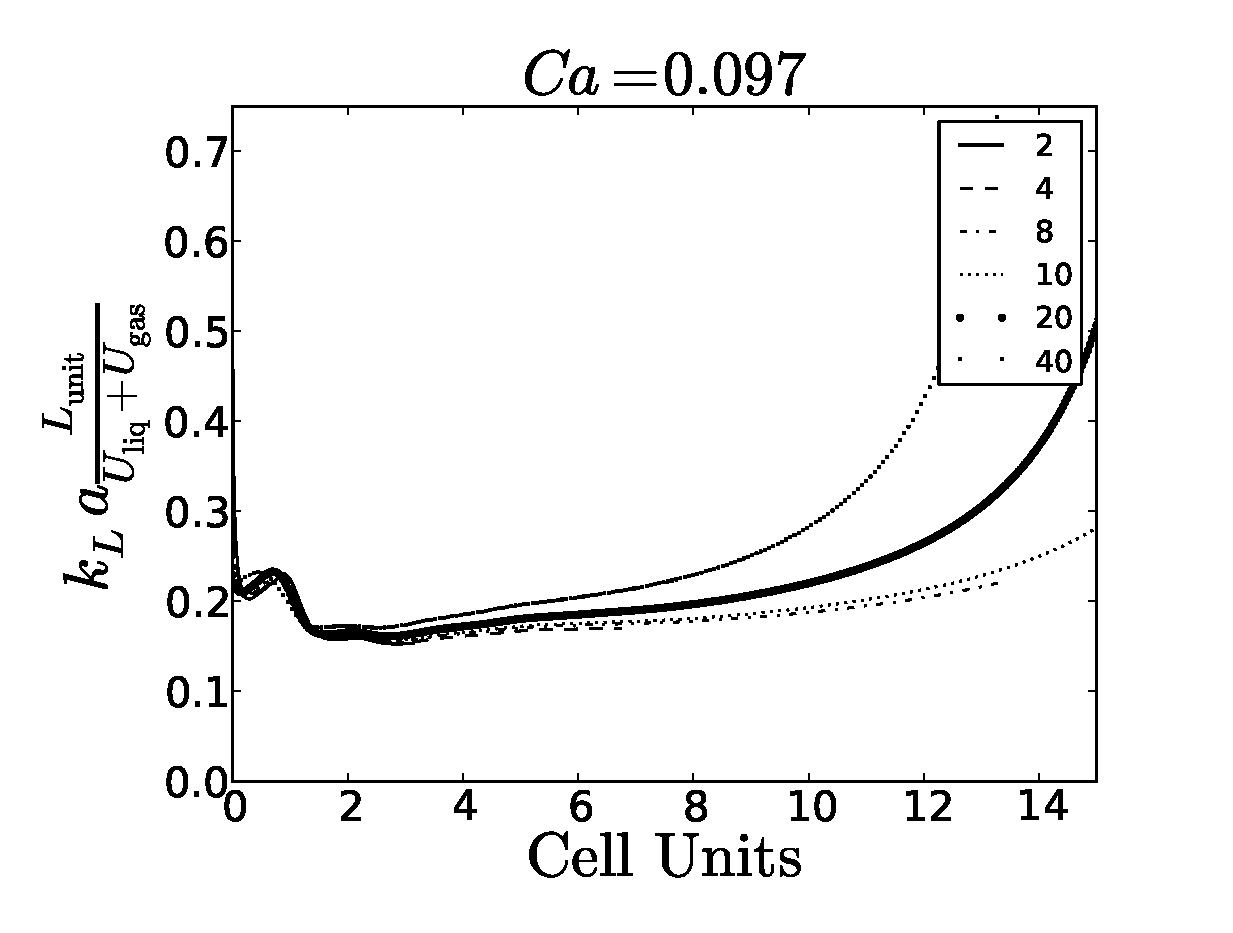
\includegraphics[width=0.5\textwidth]{Figures/vanbaten_aver_scale_ca097.eps}
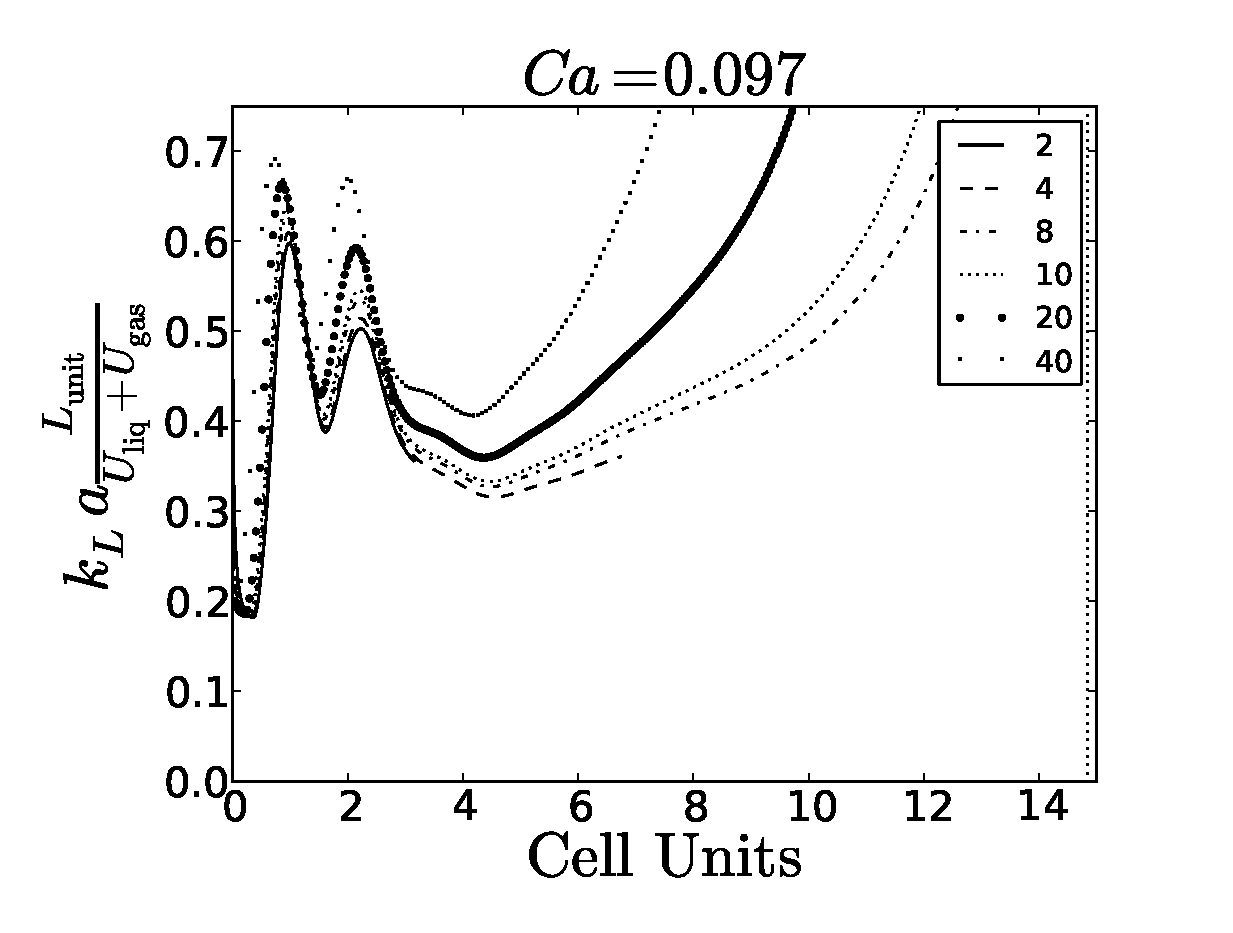
\includegraphics[width=0.5\textwidth]{Figures/vanbaten_full_scale_ca097.eps}\\
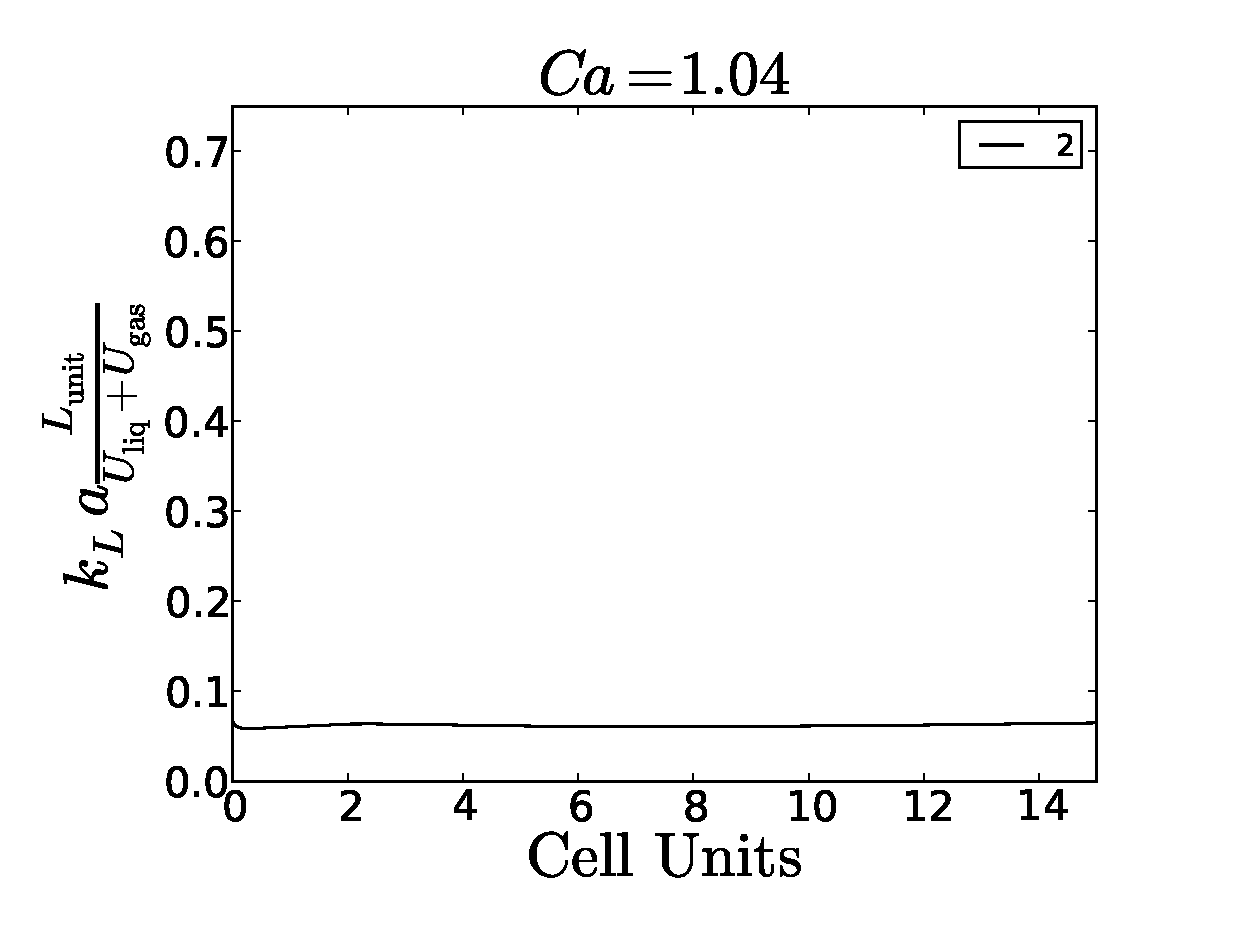
\includegraphics[width=0.5\textwidth]{Figures/vanbaten_aver_scale_ca14.eps}
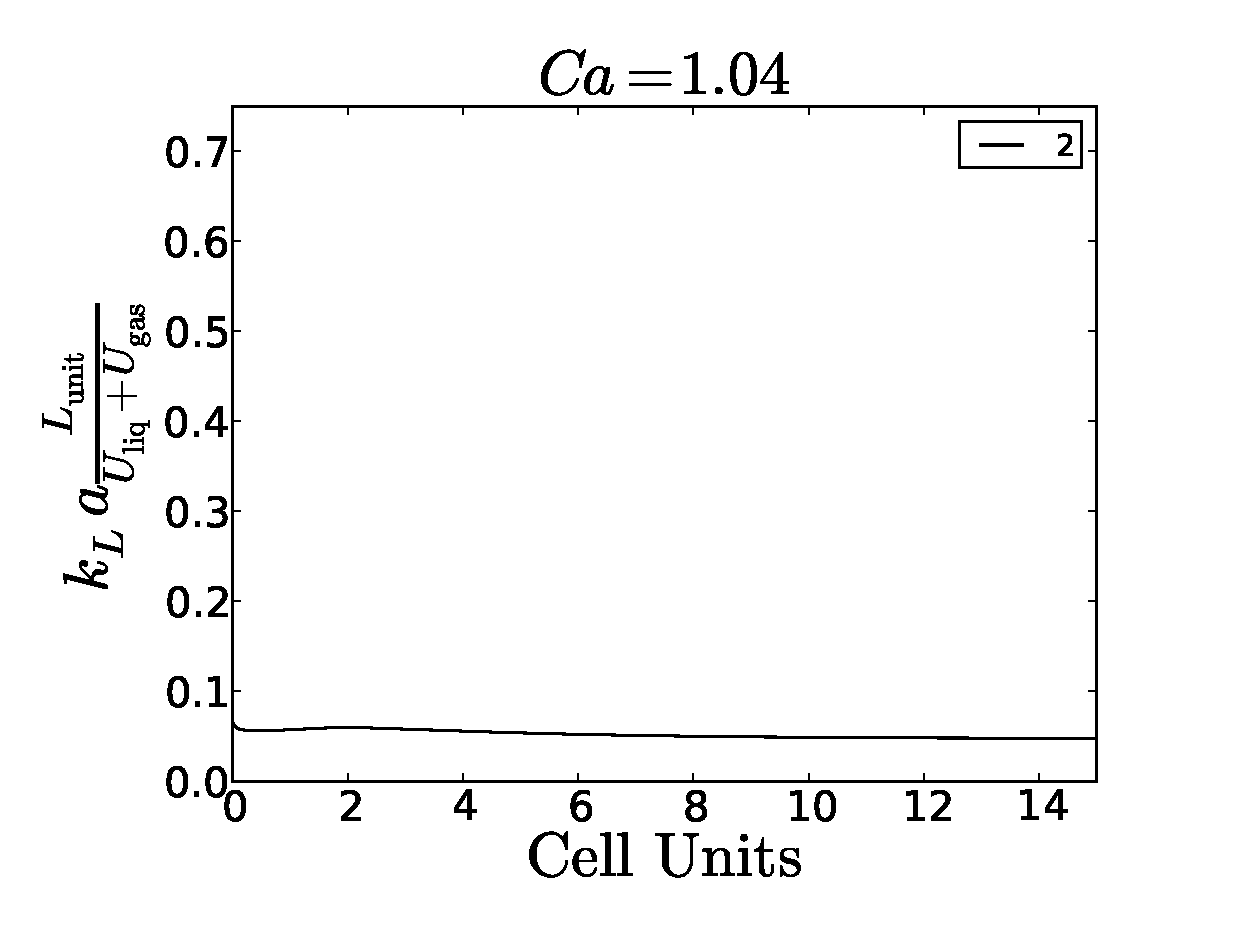
\includegraphics[width=0.5\textwidth]{Figures/vanbaten_full_scale_ca14.eps}\\
\caption{The \citet{vanbaten-circular} formulations for $Ca=0.097$ (top) and
$Ca=1.04$ (bottom) with the characteristic concentration being domain
averaged (left) and inlet/outlet flux averaged concentration (right). One can
see that \citet{vanbaten-circular} formulation is good with the characteristic concentration being
the average concentration. Moreover, the values are more close to values obtained with many cells
simulations, see Fig. \ref{fig:moving:average:ca0097}, than in comparison with periodic boundary
simulations in Section \ref{main:results:periodic}. However, the characteristic concentration
being inlet/outlet flux averaged concentration does not produce consistent results as in Section
\ref{results:periodic:inlet:outlet}.
\label{fig:vanbaten}}
\end{figure}

%\section{Open boundary conditions}
%\begin{figure}
%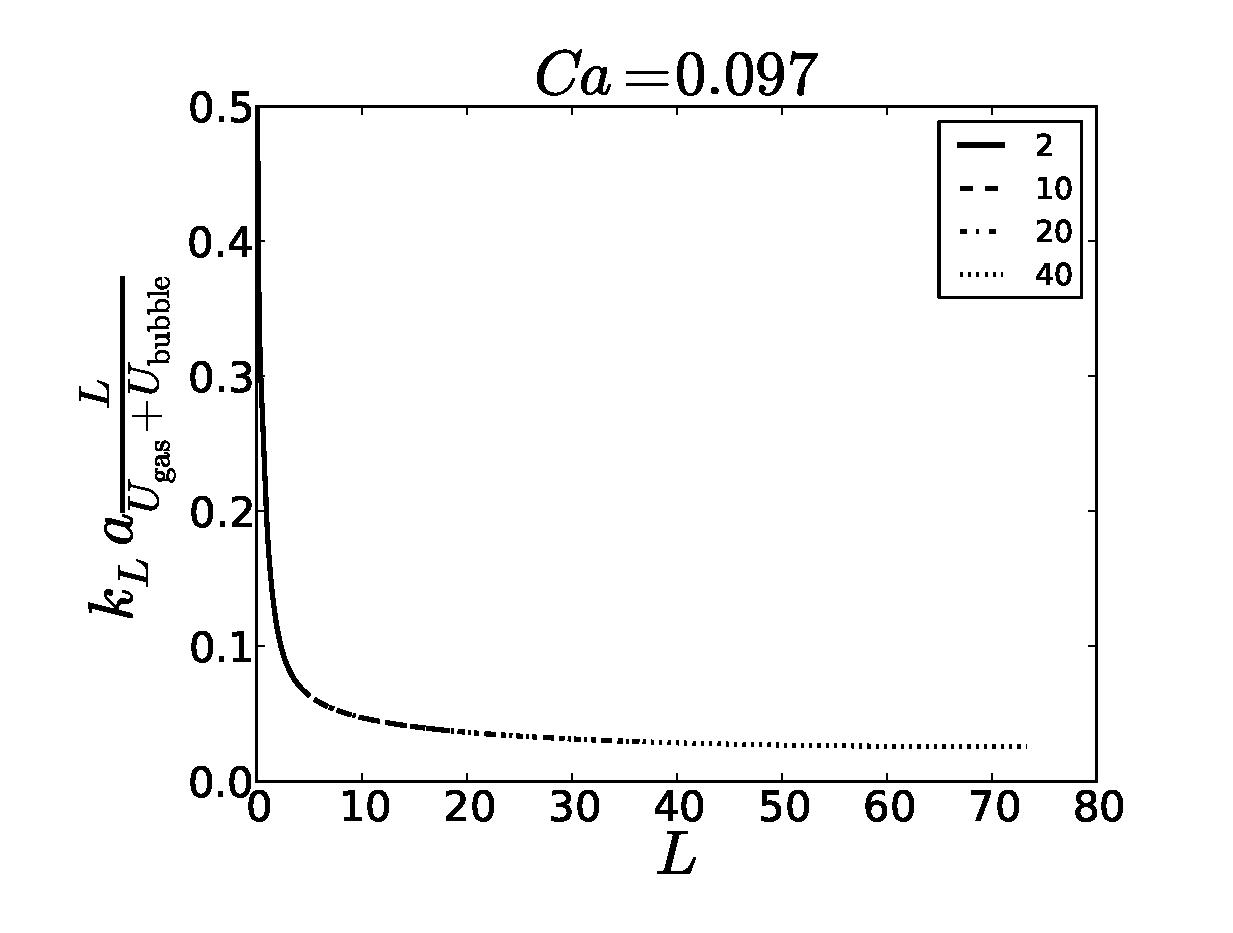
\includegraphics[width=0.5\textwidth]{Figures/jos_aver_conc_scale_ca0097.eps}
%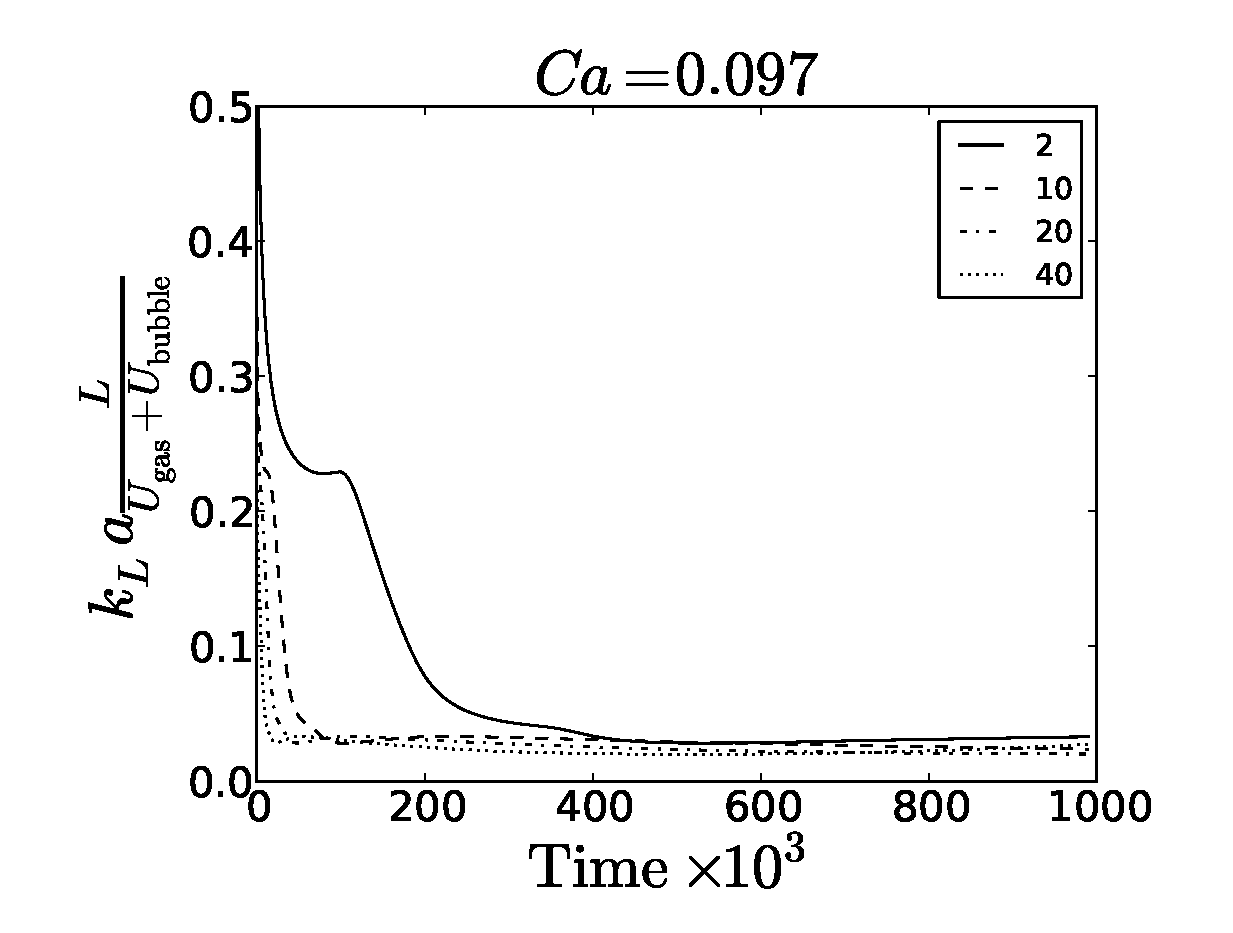
\includegraphics[width=0.5\textwidth]{Figures/jos_aver_moving_window_ca0097.eps}\\
%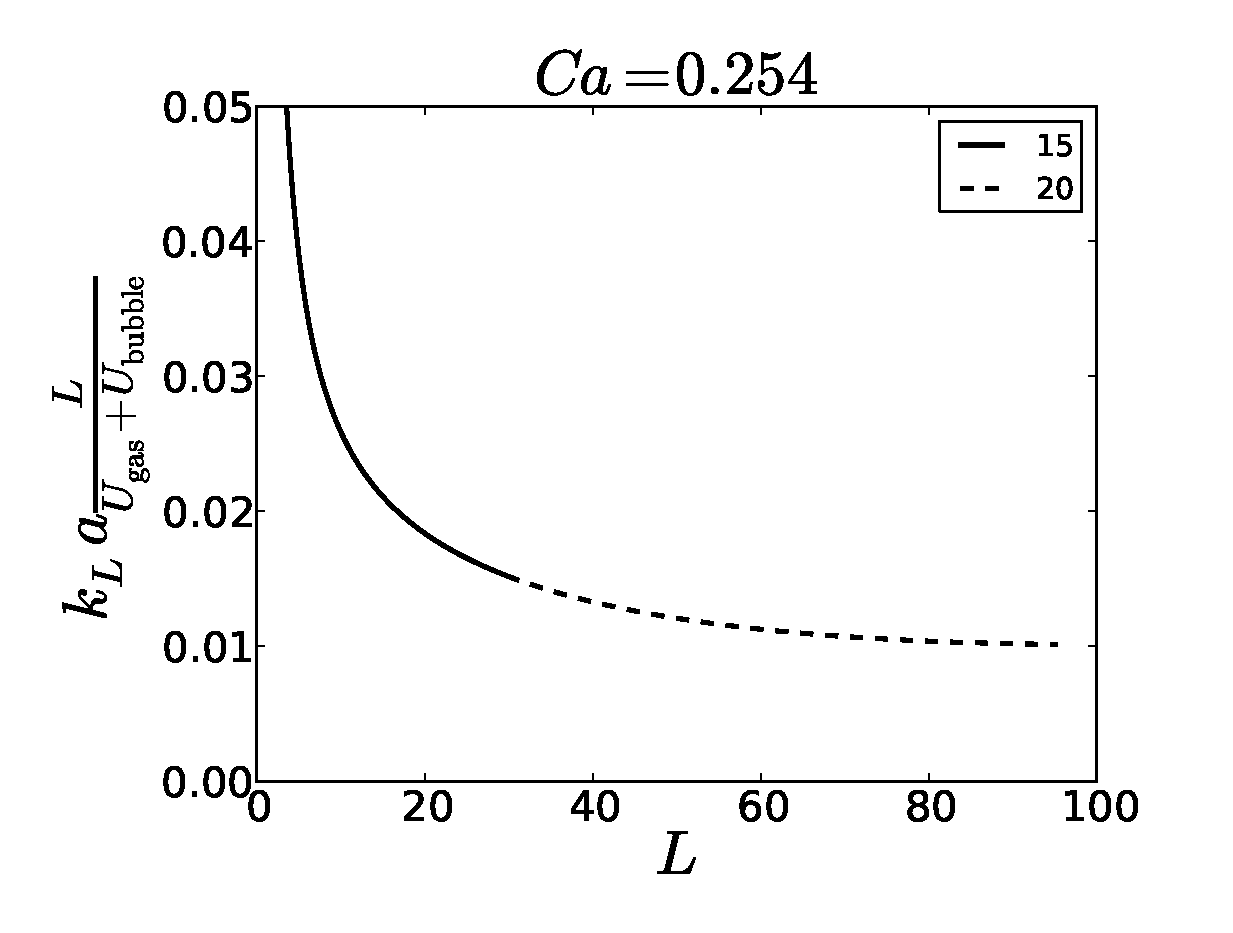
\includegraphics[width=0.5\textwidth]{Figures/jos_aver_conc_scale_ca0254.eps}
%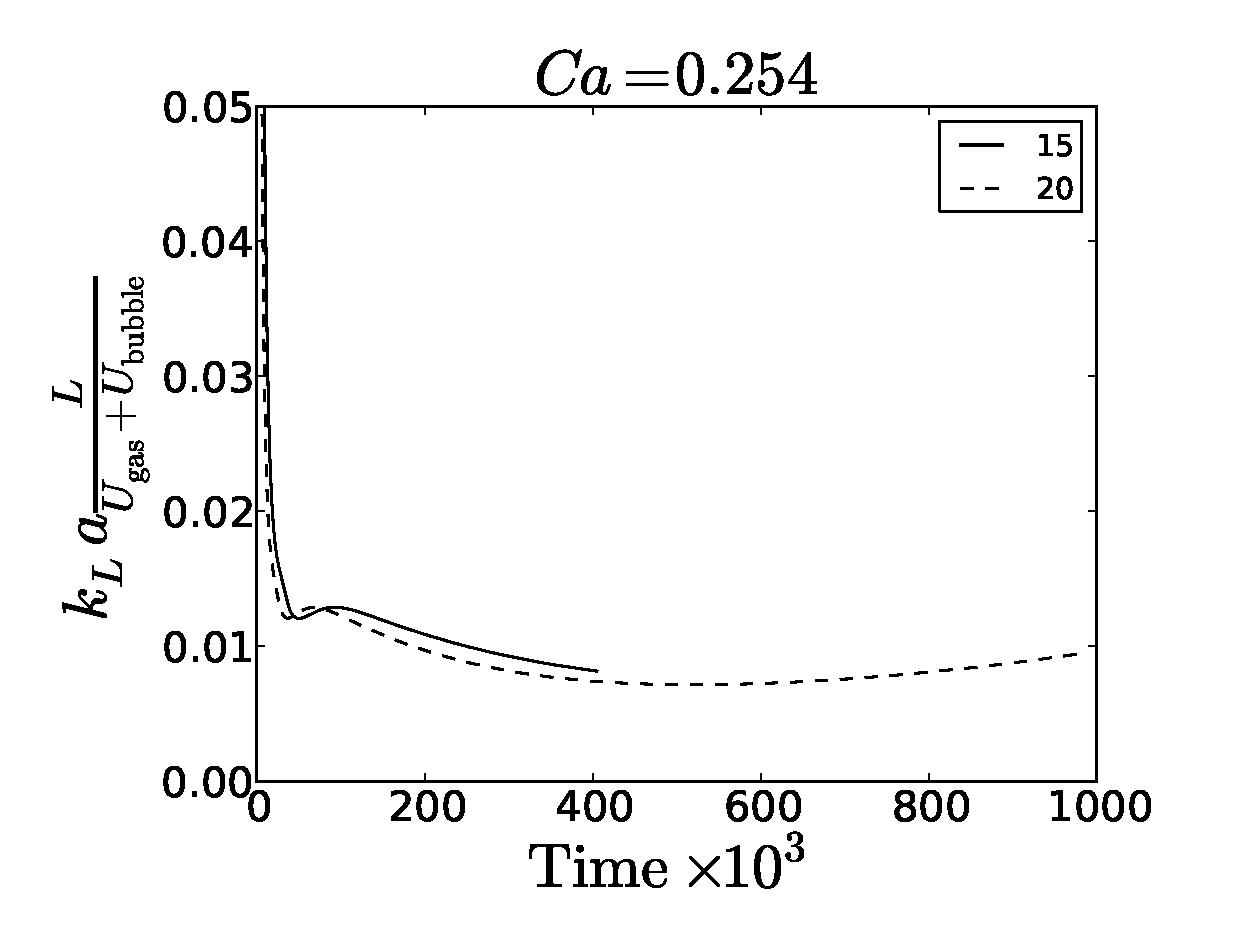
\includegraphics[width=0.5\textwidth]{Figures/jos_aver_moving_window_ca0254.eps}\\
%\caption{Open boundary conditions. \label{fig:open:boundary:jos}}
%\end{figure}
%\section{Symmetric boundary conditions}
%\begin{figure}
%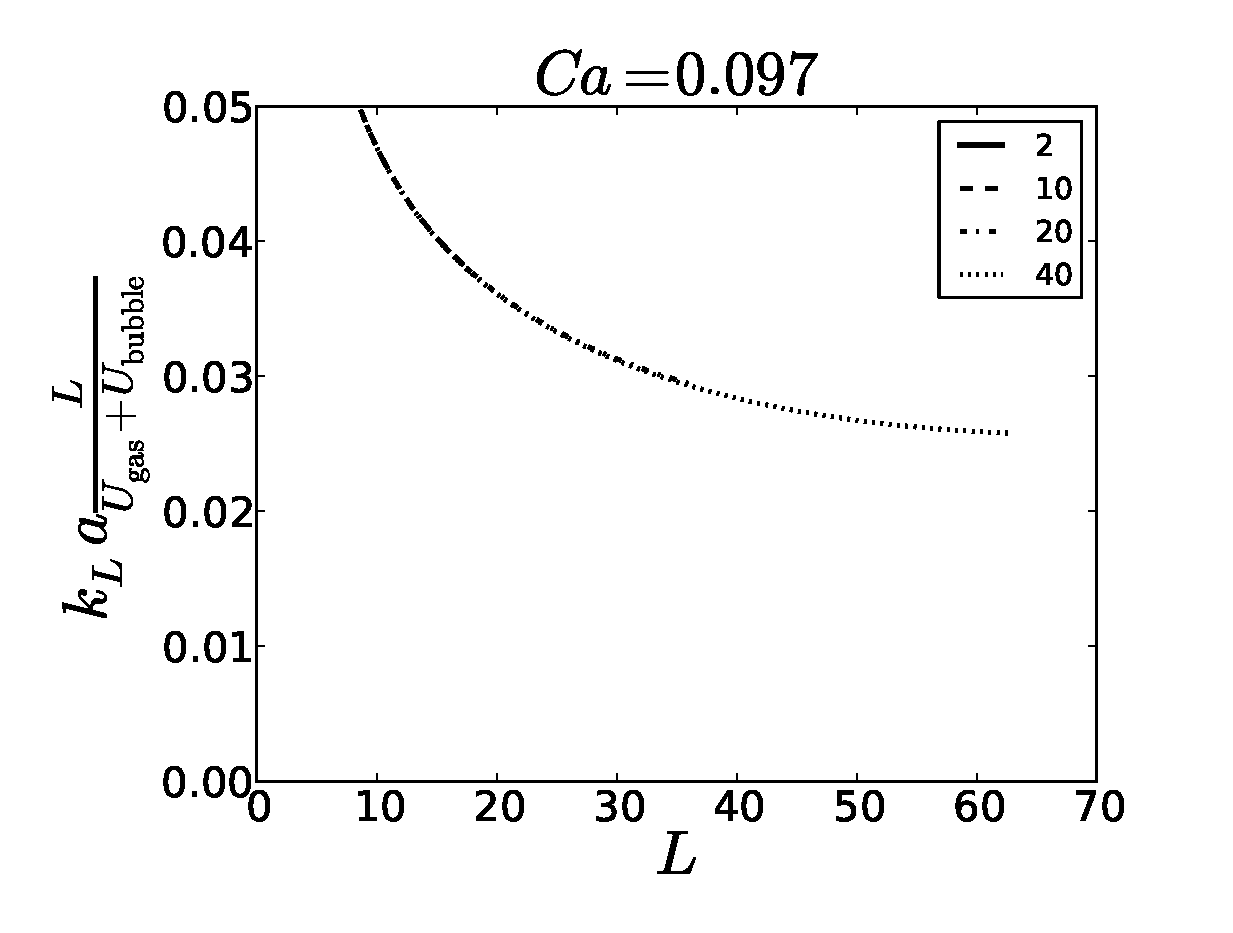
\includegraphics[width=0.5\textwidth]{Figures/sym_aver_conc_scale_ca0097.eps}
%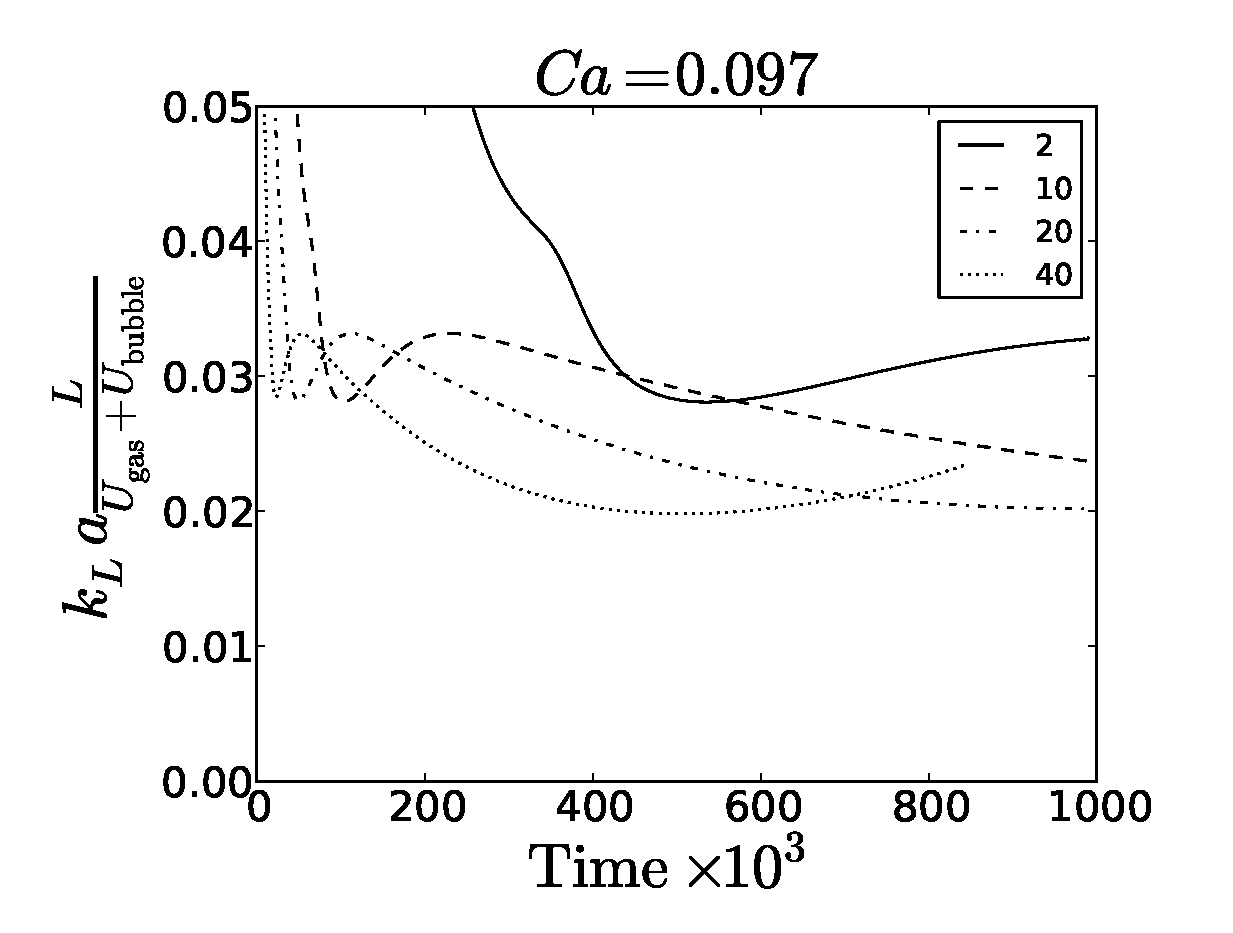
\includegraphics[width=0.5\textwidth]{Figures/sym_aver_moving_window_ca0097.eps}\\
%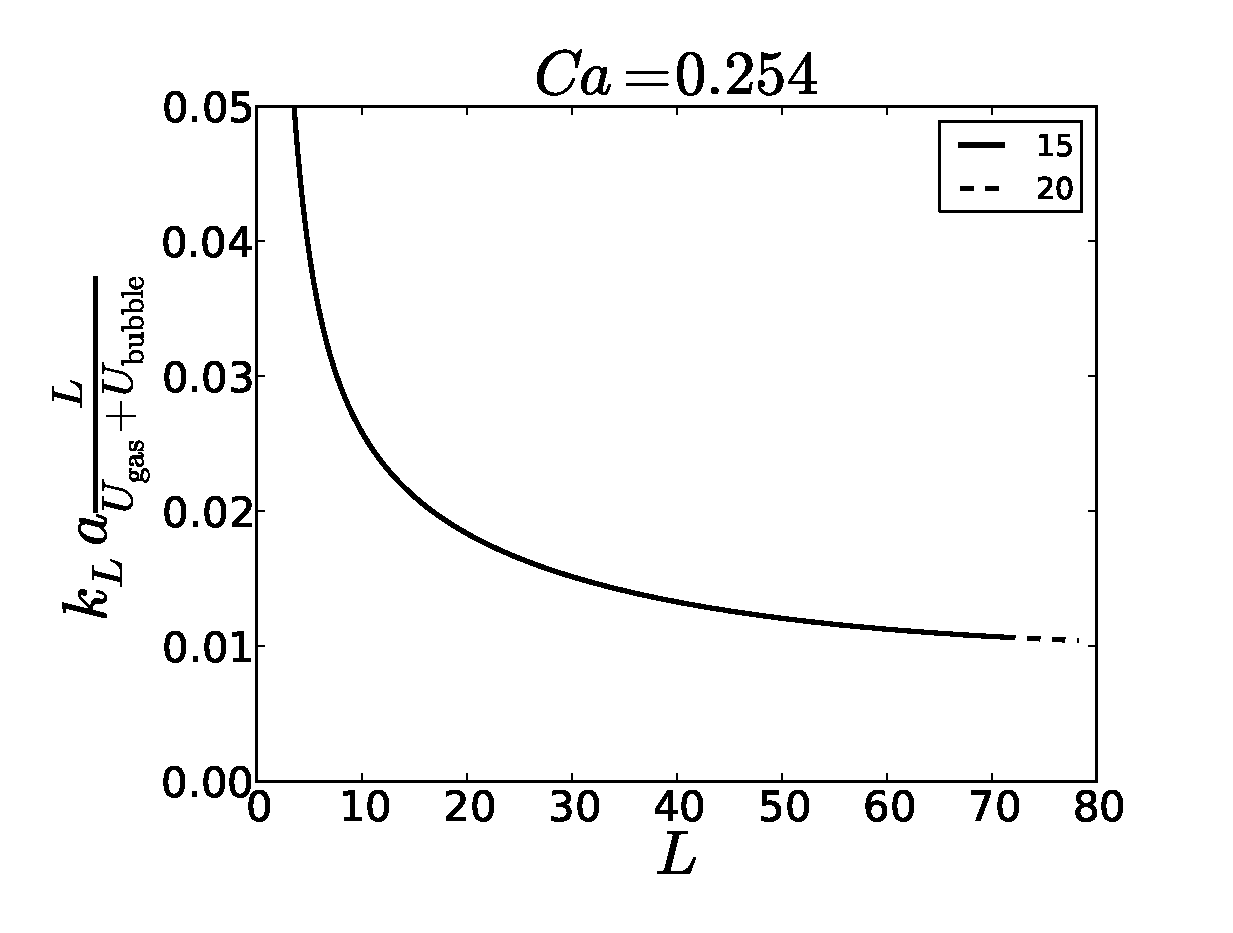
\includegraphics[width=0.5\textwidth]{Figures/sym_aver_conc_scale_ca0254.eps}
%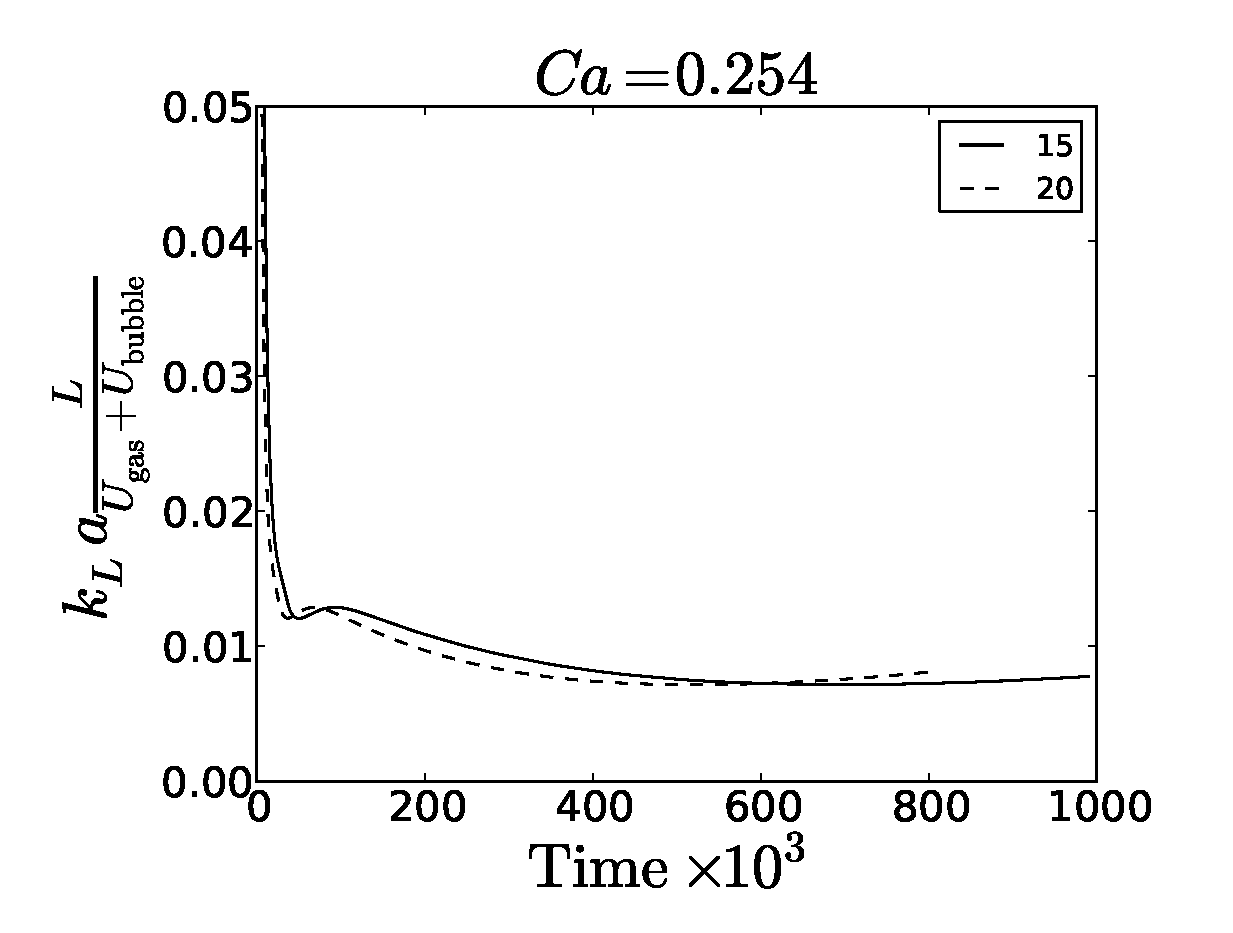
\includegraphics[width=0.5\textwidth]{Figures/sym_aver_moving_window_ca0254.eps}\\
%\caption{Symmetric boundary conditions. \label{fig:open:boundary:sym}}
%\end{figure}

\subsection{Performing a number of cell units simulations}
A few unit cells simulations naturally resemble the real experiments picture.  The idea here is
that if one have enough number of unit cells then results of internal unit cells should be
independent of boundaries and correspond to experiments. A few unit cells simulations physically
correspond to the simulation of bubble train head. If boundaries are eliminated then the average
domain characteristic should be changed in time according to Eq.
\ref{theor:continuous:mass:transfer}. It means that there is no ambiguity to choose the
characteristic concentration. The characteristic concentration is the averaged domain concentration
as it is seen in experiments.

This section studies a number of the unit cells required for the volumetric
mass transfer coefficient to be independent of boundaries. We chose two
different
velocity patterns (see Fig. \ref{fig:streamlines:tweaked:velocity} for $Ca=0.097$ and $Ca=1.04$) to
perform a few number of cells simulations. For $Ca=0.097$ we performed simulations with
$4$,$6$,$8$,$10$ number of cells, for $Ca=1.040$ only $4$,$6$,$8$ unit cells simulations.
However,
simulations with $10$ unit cells domain length produce the same results as $8$ unit cells.
Thus, it won't be covered here, especially as it requires extensive computational resources (grid is
$30000\times 200$). 

As it was discussed in the previous section we want to keep
velocity around $0.05-0.1$. The number of steps for mass to cross whole domain is
limited from above by $1.5 \frac{\lunit}{\ububble}$, which takes into the account the bulk
velocity. If $\ububble$ is taken as $0.05$ then for
the domain size $\lunit=3000$ one can obtain the following number of iteration for mass transfer to
cross the unit cell $1.5 \frac{3000}{0.05}=90000$. Therefore, $10^{6}$ time iterations are enough
for system consisting of $10$ cell units. For more accurate estimations of number of time
iterations depending
on the Peclet number one can refer to Section \ref{section:keeping:peclet}.

\subsection{$Ca=0.097$ results}
There are two characteristics we want to track for a few unit cells simulations: the average
concentration in
the unit cell with time (see Eq. \ref{theor:continuous:mass:transfer}), and the accumulated mass
rate in the domain adjusted with inlet/outlet fluxes (see Eq. \ref{main:main:main}). The former
resembles the experimental picture: if one have enough unit cells then the average domain
concentration should change in time according to Eq. \ref{theor:continuous:mass:transfer}: 
\beq
\label{moving:average}
\vol\frac{\lunit}{\ugas+\uliq}=\frac{\lunit}{\ububble (t_2
-t_1)}\ln\Bigl(\frac{C^*-C_1}{C^*-C_2}\Bigr)
\feq
The
latter is the main equation that can help to obtain the volumetric mass transfer coefficient from
mass transfer simulations with any bounary conditions (periodic boundary conditions, open
boundaries). Eq.\ref{main:main:main} can be rewritten as:
\beq
\begin{aligned}
\volnondim=\frac{\lunit}{\ugas+\ububble} \frac{V \frac{(\langle C(t_2)\rangle - \langle C(t_1)
\rangle)}{t_2-t-1}}{\dots}\\
\frac{-\int{\coutlet(\lunit,y,t^*) u(\lunit,y) \mathrm{d} y}+\int{\cinlet(0,y,t^*)
u(0,y)\mathrm{d} y}}{V (\cstar - \langle C(t^*) \rangle)},
\end{aligned}
\feq
where $t^*$ is medium time between $t_1$ and $t_2$.
%The
%argument behind this characteristic is that if the following situation is fulfilled: the continuity
%equation is satisfied then the concentration along the coordinate changes according to Eq.
%\ref{main:mass:transfer:expression}:
%\beq
%C(x)= \cstar \Bigl(1-\exp\bigl(-\vol \frac{x}{\uliq+\ugas} \bigr)\Bigr)
%\feq
%After the transition to the reference frame moving with the velocity $\ububble$, one will have the
%same continuous picture but the concentration dependency will change since velocity is changed as
%well:
%\beq
%C(x)= \cstar \Bigl(1-\exp\bigl(-\vol \frac{x}{\uliq+\ugas-\ububble} \bigr)\Bigr),
%\feq
%Thus, the volumetric mass transfer coefficient for two concentrations which are located at the
%distance $\lunit$ can be found as:
%\beqal
%&\vol \frac{\lunit}{\uliq+\ugas-\ububble}=\ln\Bigl(\frac{\cstar-C_1}{\cstar-C_2}\Bigr)\\
%&\vol
%\frac{\lunit}{\uliq+\ugas}=\frac{\uliq+\ugas-\ububble}{\uliq+\ugas}\ln\Bigl(\frac{\cstar-C_1}{
%\cstar-C_2}\Bigr)
%\feqal
%Parameters $\frac{\uliq+\ugas-\ububble}{\uliq+\ugas}$ were calculated and for representative
%Capillary numbers equal to $0.11,0.04,-0.02,-0.06,-0.10$.
%In the case of present simulations the situation is different as the reference frame is moving with
%the bubble. Thus, the correlation between adjacent cells as follows:
%\beqal
%\label{volumetric:between:adjacent:cells}
%&C_1=C(x)=C^* \Bigl(1-e^{-\vol \frac{x}{\ugas+\uliq-\ububble}}\Bigr)\\
%&C_2=C(x+L)=C^* \Bigl(1-e^{-\vol \frac{x+L}{\ugas+\uliq-\ububble}}\Bigr)\\
%&k_L\frac{L}{\ugas+\uliq-\ububble}=\frac{C^*-C_1}{C^{*}-C_2}\\
%&k_L\frac{L}{U}=\frac{C^*-C_1}{C^*-C_2},
%\feqal
%where $U=\ugas+\uliq-\ububble$. We will see later that this characteristic is really important to
%see whether the liquid slug is mixed. 
Fig. \ref{fig:unit:6} shows average concentrations in different units and $\volnondim$ based on Eq.
\ref{main:main:main} calculated for each unit for velocity
scale $10$ and  $6$ unit cells (all velocity scales produce same results). One can see that the
volumetric mass transfer cofficient is consistent for internal segments, i.e. $3-5$. One can see
that Eq. \ref{main:main:main} for a few unit cells produce the same results as periodic boundary
conditions in Section \ref{main:results:periodic}. The same dependencies
can be found for
$8$ and $10$ unit cells simulations but we do not present them here. As well we do not present $4$
units cells simulation results which are influenced by inlet and outlet boundaries. 

The non-dimensional volumetric mass transfer coefficient calculated based on Eq.
\ref{theor:continuous:mass:transfer} (averaged domain concentration changes in times) is
represented in Fig. \ref{fig:moving:average:ca0097} for different unit cells. One can see that the
results are less than the volumetric mass transfer coefficient , but consistent with the mass flux
concentration based on \citeauthor{vanbaten-circular} formulation with the characteristic
concentration being averaged domain concentration (see Section \ref{results:vanbaten}).
\begin{figure}[htb!]
%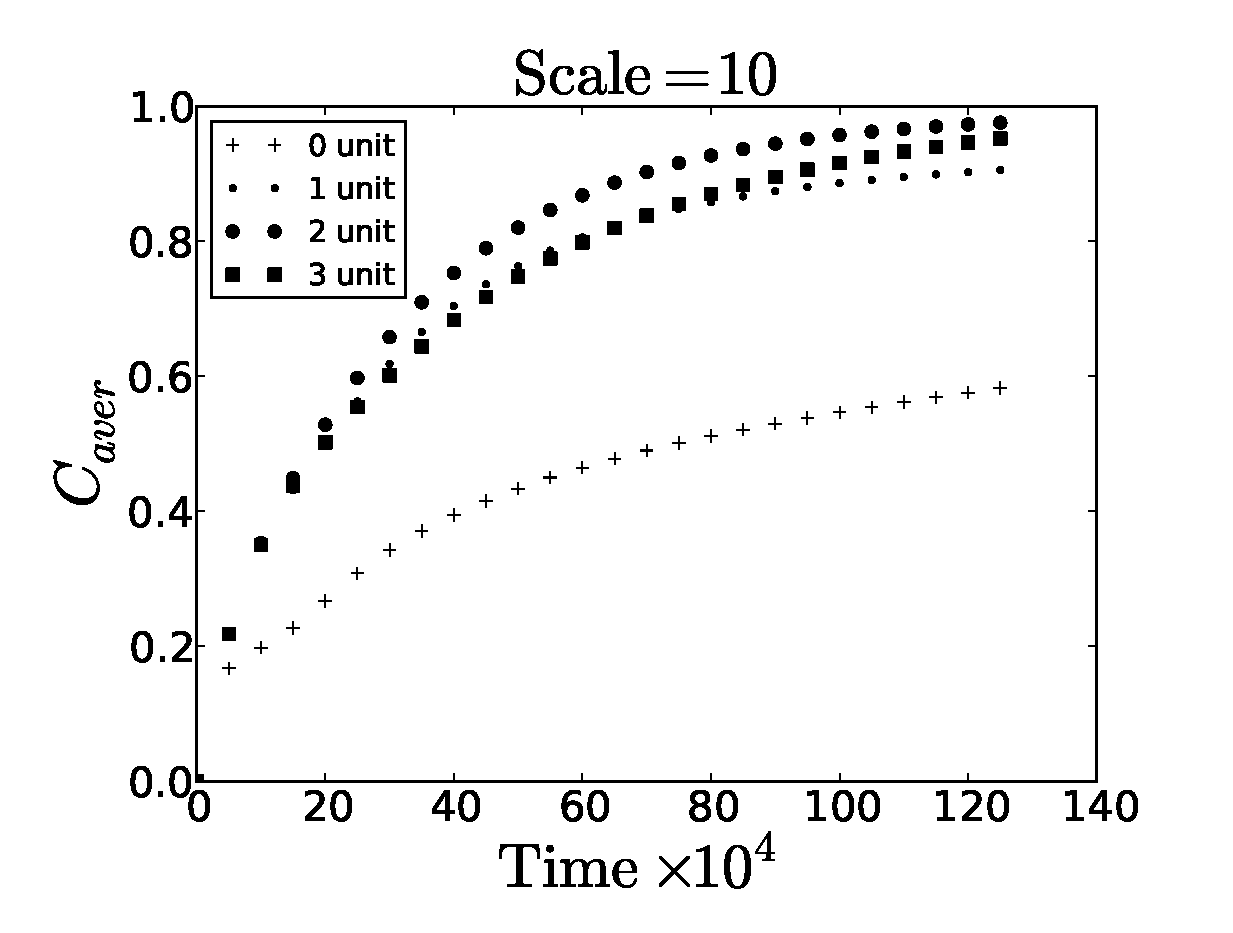
\includegraphics[width=0.5\textwidth]{Figures/aver_units4scale10.eps}\hfill
%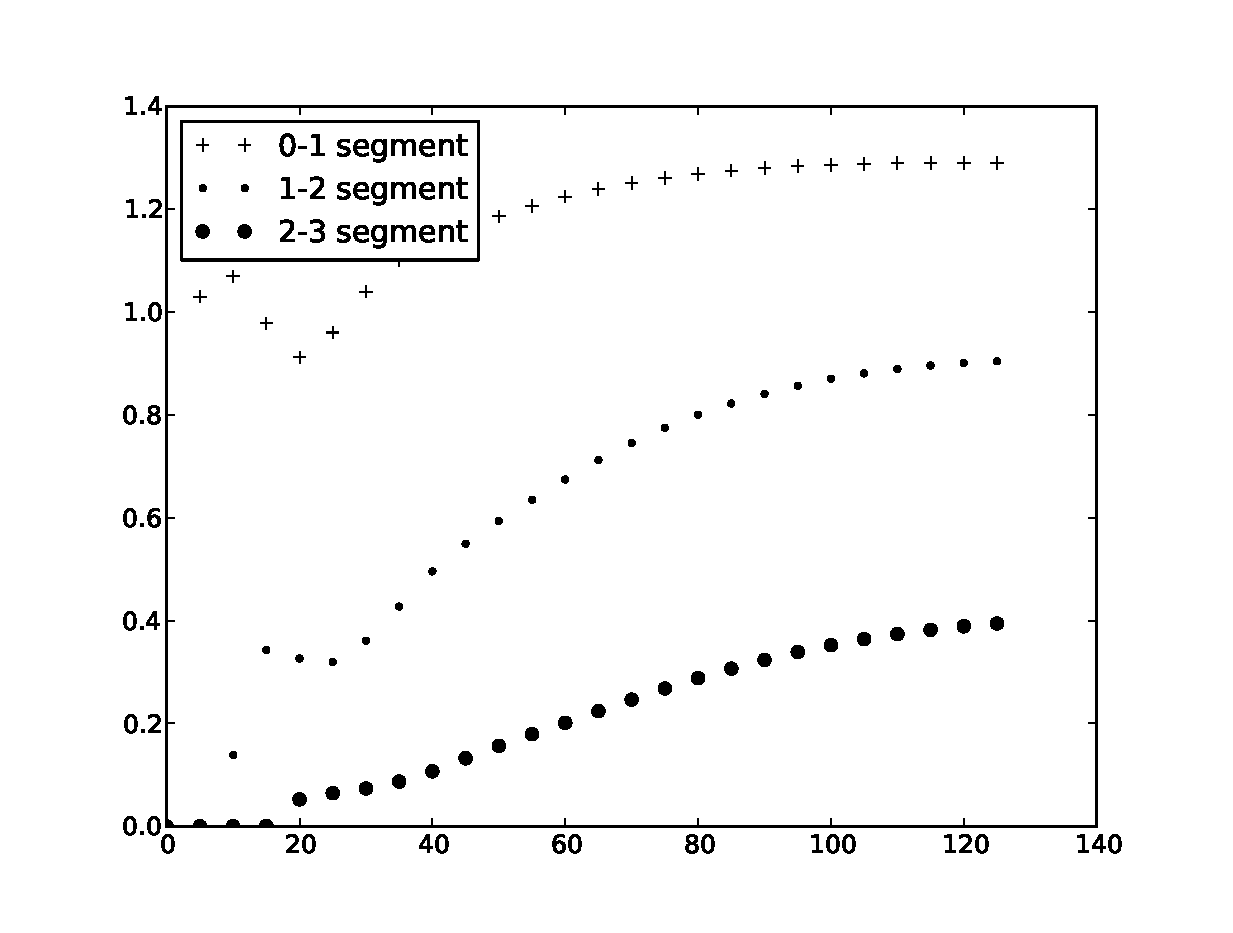
\includegraphics[width=0.5\textwidth]{Figures/coeff_units4scale10.eps}\\
%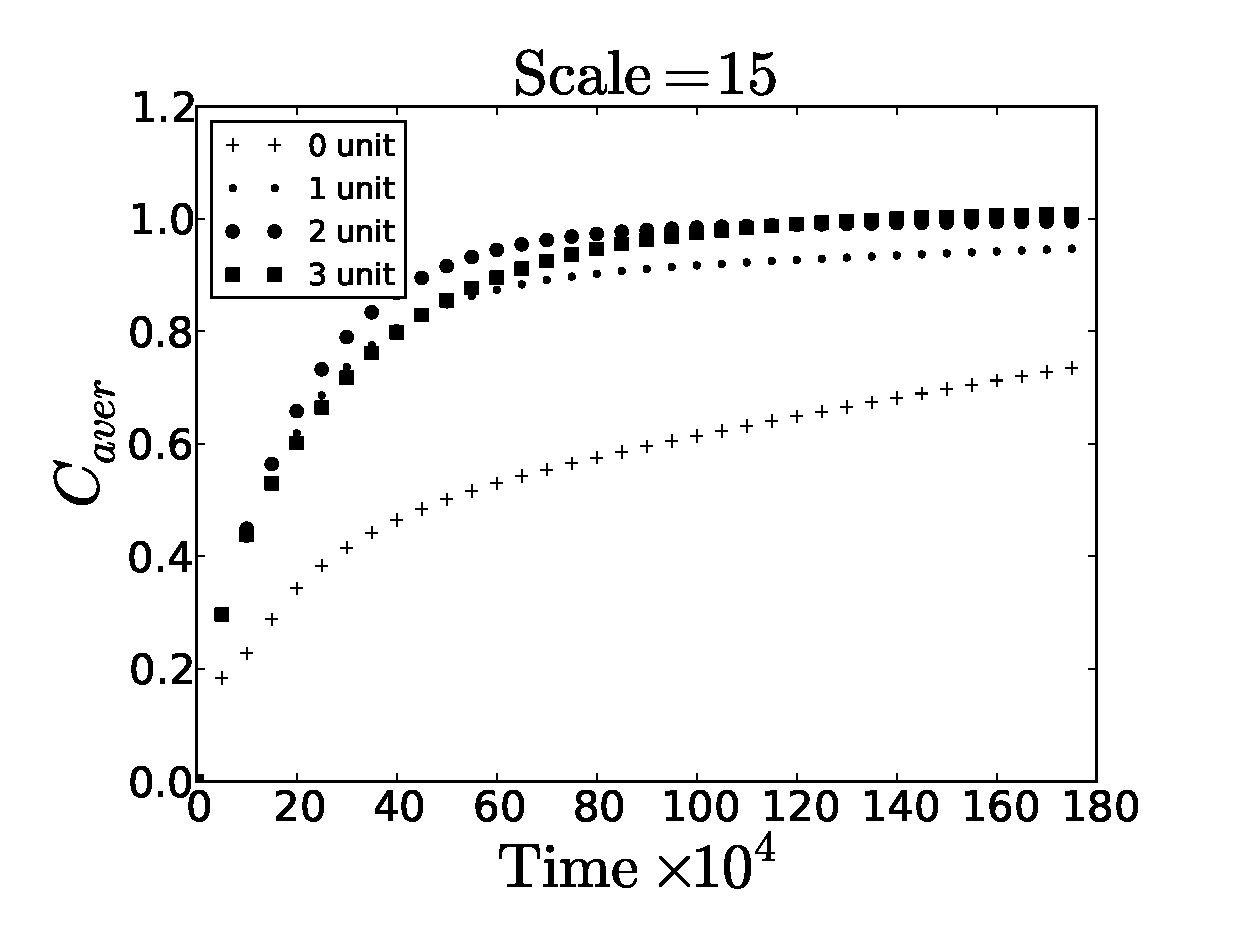
\includegraphics[width=0.5\textwidth]{Figures/aver_units4scale15.eps}\hfill
%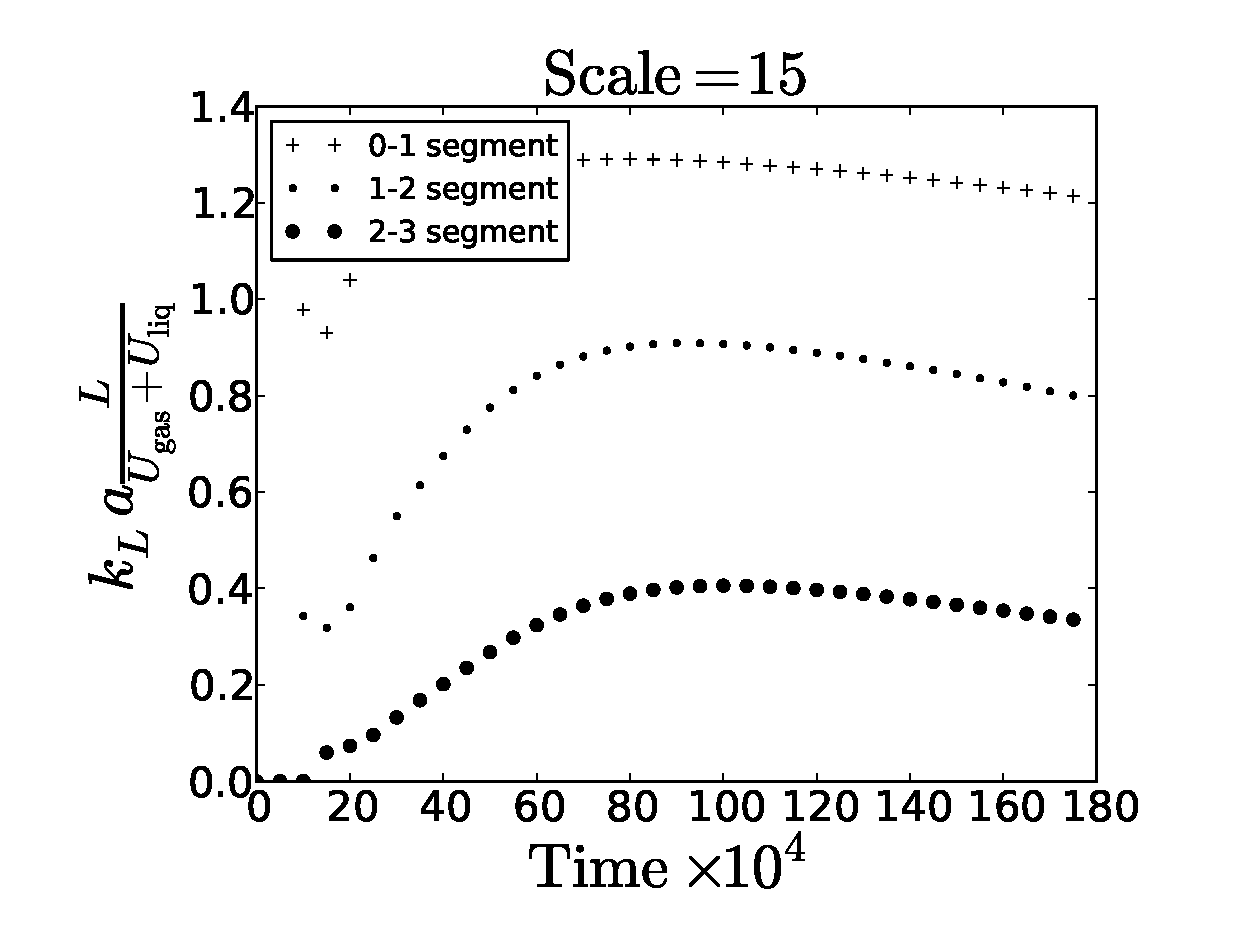
\includegraphics[width=0.5\textwidth]{Figures/coeff_units4scale15.eps}\\
\includegraphics[width=0.5\textwidth]{Figures/aver_units6scale10.eps}\hfill
\includegraphics[width=0.5\textwidth]{Figures/right_def_6scale10.eps}\\
%\includegraphics[width=0.5\textwidth]{Figures/coeff_units4scale20.eps}\\
\caption{Average concentrations (left) and volumetric coefficients (right) for $6$ units cells. The
volumetric
mass transfer coefficient is calculated based on Eq. \ref{main:main:main} and accounts for inlet
and outlet fluxes. \label{fig:unit:6}}
\end{figure}
\begin{figure}[htb!]
\includegraphics[width=0.5\textwidth]{Figures/aver_moving_window4scale10.eps}
\includegraphics[width=0.5\textwidth]{Figures/aver_moving_window6scale10.eps}\\
\includegraphics[width=0.5\textwidth]{Figures/aver_moving_window8scale10.eps}
\caption{The non-dimensional volumetric mass transfer coefficient defined in Eq.
\ref{moving:average} for $4$ (top left),$6$ (top right),$8$ cell units (bottom). Only scale
$10$ is presented since all other simulations produce the same results. One can see that $4$ unit
cells is not enough to avoid the influence of boundaries. However, the results for $6$ and $8$
unit cells are consistent and show that beginning from third unit cell the results and ending with
prelast cell results are consistent with periodic boundary simulations and
\citet{vanbaten-circular} formulations.
\label{fig:moving:average:ca0097}}
\end{figure}

\subsection{$Ca=1.040$ results}
The same correlations were examined for the different velocity pattern $Ca=1.040$ and initial
velocity $\ububble=0.055$ and initial diffusion $D=0.0008375$. If only velocity scaling is
performed then a few unit cells simulations for
this capillary number  are unstable. To improve stability we changed original Peclet number by
increasing
diffusion. The results for unit cells are the same as for $Ca=0.097$:
at least $6$ unit cells are required to be simulated to avoid the influence of boundaries. Thus,
only $6$ unit cells results are presented in Fig. \ref{fig:6:units:ca1040}, that show only the
average concentration for each unit cell. One can see that the average volume concentration come to
constant values and are not increasing with time. Thus, all the
mass generated with medium is transfered through the boundaries. This is the indication that the
liquid slug is not mixed. Note that the periodic boundary conditions can not show whether the
liquid slug is mixed or not, since the averaged domain concentration is always increasing in time. 
Thus, the volumetric mass transfer coefficient $\volnondim$ can be calculated according to the
definition, Eq. \ref{main:main:main}:
\beq
\label{inlet:outlet:spatial:location}
\vol =
\frac{\dot{m}-\int{\coutlet(y)u(\lunit,y)\mathrm{d}y}+\int{\cinlet(y)u(\lunit,y)\mathrm{d}y}}{V
\Delta C},
\feq 
where $V$ is the unit cell volume, $\Delta C$ is the concentration difference between the bubble
surface concentration $\cstar$ and the averaged liquid domain concentration $\langle
C(t)\rangle$. There is no accumulated mass in the domain. Thus, $\dot{m}=0$. As periodic boundary
conditions this case is another extreme limit of Eq. \ref{main:main:main}. Note that to calculate
the volumetric mass transfer coefficient one needs only the spatial information and does not
require the knowledge of how concentration is changed in time. 

Fig. \ref{fig:periodic:ca1040}
(bottom) shows the volumetric mass transfer coefficient, based on spatial calculations of
inlet/outlet concentrations. One can see that the volumetric mass transfer coefficient is close to
the calculated volumetric mass transfer coefficient using the time averaged approach and periodic
boundaries one unit cells simulations. 
\begin{figure}[htb!]
\begin{center}
\includegraphics[width=0.5\textwidth]{Figures/aver_units6scaleu2scaled5.eps}
\end{center}
%\includegraphics[width=0.5\textwidth]{Figures/novortex6scaleu2scaled5.eps}\\
\caption{Results for $6$ unit cells. The Peclet number equals to $Pe=2644$.
One can see that average concentrations reach certain number and stay.
That means whatever was
generated by medium is transfered through the outlet
boundary. O This is the indication that the tracer in the slug is not
mixed and the volumetric mass transfer coefficient, $\volnondim$, can be
calculated using the spatial approach, see Fig.
\ref{fig:periodic:ca1040}.\label{fig:6:units:ca1040}}
\end{figure}
The volumetric mass transfer coefficient with periodic boundary simulations for $Pe=2644$ (velocity
scale $2$, diffusion scale $10$) and time dependent, Eq. \ref{theor:continuous:mass:transfer},
average volumetric mass transfer coefficient are presented in Fig. \ref{fig:periodic:ca1040}. Note
that they coincide. Therefore, for certain hydrodynamic patterns one can easily convert time
domain to the spatial domain calculations.
\begin{figure}
\includegraphics[width=0.5\textwidth]{Figures/volume_ca_104_scaleu2scaled5.eps}
\includegraphics[width=0.5\textwidth]{Figures/aver_moving_window6scaleu2scaled5.eps}\\
\includegraphics[width=0.5\textwidth]{Figures/flux_moving_window6scaleu2scaled5.eps}\\
\caption{The periodic (top left, $1$ unit cell, Eq. \ref{theor:continuous:mass:transfer}), unit
cells averaged domain concentrations in time (top right, $6$ unit cells, Eq.
\ref{theor:continuous:mass:transfer}), and spatial location
(bottom, $6$ unit cells, Eq. \ref{inlet:outlet:spatial:location}) calculated  volumetric mass
transfer
coefficients. One can see that they all coincide. However, the periodic boundary conditions based
calculations produce a bit overestimated volumetric mass transfer
coefficient. As well one can see that the averaged domain concentration simulations (top right)
reach the steady volumetric concentrations fast and after that start decaying. It is not convenient
to use them in practical cases for not mixed slug, i.e. $Ca>0.7$. \label{fig:periodic:ca1040}}
\end{figure}

\subsection{Experiment and Analytical correlations comparison}
The goal of this paper is not to compare with the experiment correlations, but give the
procedure to perform numerical simulationsrof  in the lattice Boltzmann framework. However, the
small comparison is performed.
Unfortunately the experiments to the best authors' knowledge measuring the mass flux for infinite
width  bubbles flowing between parallel plates are absent. However, one of interesting
correlations for the mass transfer volumetric coefficient was presented by
\citet{yue-mass} for three-dimensional microchannel geometries:
\beqal
&\vol=\frac{2}{d_h}\Bigl(\frac{D \ububble}{\lbubble+\lslug}\Bigr)^{0.5}
\Bigl(\frac{\lbubble}{\lbubble+\lslug}\Bigr)^{0.3}\\
&\vol \frac{\lunit}{\ugas+\uliq}=2\frac{\lunit}{d_h} \Bigl(\frac{D 
}{\lunit (\ububble+\ugas)} \frac{\ububble}{\ugas+\uliq}\Bigr)^{0.5}
\Bigl(\frac{\lbubble}{\lbubble+\lslug}\Bigr)^{0.3} \propto Pe^{-\frac{1}{2}}\\
&\vol \frac{\lunit}{\ugas+\uliq}=2\frac{\lunit}{d_h} \Bigl(\frac{D 
}{\lunit (\ububble+\ugas)} \frac{\ububble}{\ugas+\uliq}\Bigr)^{0.5}
\Bigl(\frac{\lbubble}{\lbubble+\lslug}\Bigr)^{0.3} \propto Pe^{-\frac{1}{2}}
\feqal
One can see that approximately the volumetric mass transfer correlation should be proportional to
$Pe^{-0.5}$. As well one can use analytical estimations for the volumetric mass transfer
coefficient calculated using Higbie penetration theory \cite{higbie}. One can show following works
\cite{irandoust,vanbaten-circular} that the analytical expression for the flow between plats has
the following form:
\beq
\label{vanbaten:analytical:expresssion}
\begin{aligned}
\volnondim=&\frac{\lunit}{\ugas+\uliq}\Bigl(4 \sqrt{D \ububble}{\pi}
\frac{\sqrt{\lbubble-H (1-2\delta)}}{\lunit H}\\
&+2 \sqrt{2} \sqrt{D \ububble} \frac{\sqrt{H
(1-2\delta)}}{\lunit H}\Bigr),
\end{aligned}
\feq
where $H$ is the channel height, $\delta$ is the film thickness.

Fig. \ref{fig:volume:mass:coefficient} shows a comparison between corelation by
\citet{yue-mass}, analitical expression, Eq. \ref{vanbaten:analytical:expresssion} and the current
simulations coefficients presented in Table
\ref{table:steady:state:average}. The coefficients are close to each other, especially given that
the correlation by \citet{yue-mass} is for three-dimensional cases. The fitting procedure showed
that the power of
the Peclet number $Pe$ is $-0.50038$ which is close to $-0.5$. 
\begin{figure}[htb!]
\includegraphics[width=\textwidth]{Figures/correlations_comparison.eps}
\caption{Comparison between correlation by \citet{yue-mass}, analytical correlation following work
\cite{irandoust} and mass transfer coefficient based
on periodic boundary conditions. The fitting curve is proportional to $Pe^{-0.5}$ which corresponds
to all correlations. As well one can see that the deviation from the analytical expression becomes
larger because the analytical expression does not account for the velocity pattern and a bubble
shape change.\label{fig:volume:mass:coefficient}}
\end{figure}

\section{Conclusion}
This work examines a way to calculate the volumetric mass transfer coefficient in the framework of
the lattice Boltzmann method. Overall, the easiest recipe is to perform periodic boundary
conditions simulations and calculate the volumetric mass transfer coefficient based on the averaged
domain concentration through any formulation as they produce consistent results. The best accuracy
is achieved with formulations based on the mass difference or on the averaged domain concentrations
taken in different times, Eq. \ref{theor:continuous:mass:transfer}. Eq.
\ref{theor:average:concentration:time} gives a bit overestimated volumetric mass transfer
coefficient. Formulation of
\citet{vanbaten-circular} is inconsistent if one takes the inlet/outlet flux averaged concentration
to be characteristic concentration. A few unit cells simulations are harder to perform, but they
have indicator of how well the liquid slug is mixed. As well, for velocity patterns for $Ca\geq
0.7$ simulations with a few unit cells allow to calculate the volumetric mass transfer
coefficient based on the spatial location, not time averaged values used in all other
approaches. Finally, a sample of results was
compared with the experimental correlation of \citet{yue-mass} and shows a good agreement. 
\appendix
\section{Analytical solution for parabolic profile with zero velocity gradient at $0$}
\label{appendix:zero:gradient}
The problem is defined in terms of PDE as follows: 
\beq
\label{diffusion:zero:gradient:start}
\begin{aligned}
&\frac{\partial C}{\partial x} U(y)=D\frac{\partial^2 C}{\partial y^2}\\
&C(0,y)=C_0,\, C(x,0)=\cstar,\, \frac{\partial C}{\partial y }(x,\delta)=0\\
&U(y)=U_0 \Bigl(\frac{y}{\delta}\Bigr)^2
\end{aligned}
\feq
The non-dimensional parameters are introduced:
\beq
\begin{aligned}
&\frac{\partial C}{\partial \frac{x}{\delta}} \frac{U_0}{\delta}
\Bigl(\frac{y}{\delta}\Bigr)^2=\frac{D}{\delta^2}\frac{\partial^2 C}{\partial
\frac{y^2}{\delta^2}}\\
&C(0,y)=C_0,\, C(x,0)=\cstar,\, \frac{\partial C}{\partial y }(x,\delta)=0\\
\end{aligned}
\feq
After a change of variables:
\beq
\begin{aligned}
&\zeta=\frac{x}{\delta} \frac{D}{U_0 \delta}=\frac{1}{Pe}\frac{x}{\delta}\\
&\xi=\frac{y}{\delta},
\end{aligned}
\feq 
Eq. \ref{diffusion:zero:gradient:start} with boundary conditions becomes as follows:
\beq
\label{diffusion:zero:gradient:middle}
\begin{aligned}
&\frac{\partial C}{\partial \zeta}\xi^2=\frac{\partial^2 C}{\partial \xi^2}\\
&C(0,\xi)=C_0\\
&C(\zeta,0)=\cstar\\
&\frac{\partial C}{\partial \xi}(\zeta,1)=0\\
\end{aligned}
\feq 
Still Eq. \ref{diffusion:zero:gradient:middle} cannot be solved with the separation of variables as it requires homogenous
boundary conditions. Thus, let us introduce the new variable, $\Theta=C-\cstar$, which makes the system to be with homogenous boundary conditions:
\beq
\begin{aligned}
&\frac{\partial \Theta}{\partial \zeta}=\frac{1}{\xi^2}\frac{\partial^2 \Theta}{\partial \xi^2}\\
&\Theta(0,\xi)=C_0-\cstar \\
&\Theta(\zeta,0)=0,\, \partial_{\xi}\Theta(\zeta,1)=0\\
\end{aligned}
\feq 
This equation can be solved by separation of variables if the solutions is represented as the
multiplication of two functions $\Theta(\zeta,\xi)=X(\zeta)Y(\xi)$:
\beq
\begin{aligned}
&\frac{\mathrm{d} X(\zeta)}{\mathrm{d} \zeta}Y(\xi)=\frac{X(\zeta)}{\xi^2}\frac{\mathrm{d^2}
Y(\xi)}{\mathrm{d}\xi^2}\\
&\frac{1}{X(\zeta)}\frac{\mathrm{d} X(\zeta)}{\mathrm{d} \zeta}=\frac{1}{\xi^{2} Y(\xi)}
\frac{\mathrm{d^2} Y(\xi)}{\mathrm{d}\xi^2}
\end{aligned}
\feq
The left and right parts depend on different variables. Therefore to be equal to each other both
parts shall equal to constant, say $-m^4$. Thus, the separation of the variables leads to two ODEs:
\begin{equation*}
\begin{aligned}
&\frac{\mathrm{d}X(\zeta)}{\mathrm{d}\zeta}=-m^4 X(\zeta)\\
&\frac{\mathrm{d^2}Y(\xi)}{\mathrm{d}\xi^2}+m^4 \xi^2 Y(\xi)=0\\ 
\end{aligned}
\end{equation*}
The solution of the first equation is the exponential function:
\beq
X(\zeta)=\exp(-m^4 \zeta)\\
\feq
The solutions of the second equation are two hypergeometric function which can be expressed through
the Bessel functions \cite{abramowitz}:
\beq
\begin{aligned}
&Y_1=\sqrt{\xi}J_{\frac{1}{4}}\Bigl(\frac{m^2 \xi^2}{2}\Bigr)\\
&Y_2=\sqrt{\xi}J_{-\frac{1}{4}}\Bigl(\frac{m^2 \xi^2}{2}\Bigr)\\
&Y'_1=m^2 \xi^{3/2} J_{-\frac{3}{4}}\Bigl(\frac{m^2 \xi^2}{2}\Bigr)\\
&Y'_2=m^2 \xi^{3/2} J_{\frac{3}{4}}\Bigl(\frac{m^2 \xi^2}{2}\Bigr)\\
\end{aligned}
\feq
The solution is the summation of two functions:
\begin{equation*}
Y(x)=C_1 Y_1(x)+C_2 Y_2(x). 
\end{equation*}
One can find coefficients from the boundary conditions:
\beq
\begin{aligned}
&Y(0)=0=C_1 Y_1(0)+C_2 Y_2(0)\\
&Y_1(0)=0,\,Y_2(0)=\frac{\sqrt{2}}{\sqrt{m} \Gamma(3/4)}\, C_2=0\\
&Y'(1)=0=C_1 Y'_1(1)+C_2 Y'_2(1)=C_1 Y'_1(1)\\
&J_{-\frac{3}{4}}\Bigl(\frac{m^2}{2}\Bigr)=0
\end{aligned}
\feq
Therefore one needs to find zeros of $J_{-\frac{3}{4}}\Bigl(\frac{m^2}{2}\Bigr)$. To give some
numerical values:
$m_1=1.454997085$, $m_2=2.927133004$, $m_3=3.857578101$, $m_4=4.601777732$, $m_5=5.240824067$.
Therefore, the solution in a general form is represented as:
\beq
\Theta(\zeta,\xi)=\sum_m{C_m \sqrt{\xi} J_{\frac{1}{4}}\Bigl(\frac{m^2
\xi^2}{2}\Bigr)\exp(-m^4 \zeta)}
\feq
To find unknown coefficients $C_m$ one needs to substitute the expression above to the initial
condition:
\beq
\Theta(0,\xi)=C_0-\cstar=\sum_m{C_m \sqrt{\xi}J_{\frac{1}{4}}\Bigl(\frac{m^2
\xi^2}{2}\Bigr)}\\
\feq
Using the Stourm-Liouville theorem one can multiply by $\xi^{5/2}
J_{\frac{1}{4}}\Bigl(\frac{m^2 \xi^2}{2}\Bigr)$ and integrate left and right parts of the equation:
\beq
\begin{aligned}
&\bigl(C_0-\cstar\bigr) \int_{\xi=0}^{1}{\xi^{5/2} J_{\frac{1}{4}}\Bigl(\frac{m^2
\xi^2}{2}\Bigr)\mathrm{d}\xi}=C_m\int_{\xi=0}^{1}{\xi^3 J_{\frac{1}{4}}^2\Bigl(\frac{m^2
\xi^2}{2}\Bigr)\mathrm{d}\xi}\\
&C_m = (C_0-\cstar ) \frac{\int_{\xi=0}^{1}{\xi^{5/2} J_{\frac{1}{4}}\Bigl(\frac{m^2
\xi^2}{2}\Bigr)\mathrm{d}\xi}}{\int_{\xi=0}^{1}{\xi^3 J_{\frac{1}{4}}^2\Bigl(\frac{m^2
\xi^2}{2}\Bigr)\mathrm{d}\xi}}
\end{aligned}
\feq
Therefore, the overall solution is specified as:
\beq
\begin{aligned}
&C(x,y)=\cstar+\sum_{m}{C_m
\sqrt{\frac{y}{\delta}}J_{\frac{1}{4}}\Bigl(\frac{m^2}{2}\frac{y^2}{\delta^2}\Bigr)\exp\Bigl(-\frac{
m^4 } { Pe }
\frac { x }{\delta}\Bigr)}\\
&C_m = (C_0-\cstar) \frac{\int_{\xi=0}^{1}{\xi^{5/2} J_{\frac{1}{4}}\Bigl(\frac{m^2
\xi^2}{2}\Bigr)\mathrm{d}\xi}}{\int_{\xi=0}^{1}{\xi^3 J_{\frac{1}{4}}^2\Bigl(\frac{m^2
\xi^2}{2}\Bigr)\mathrm{d}\xi}}
\end{aligned}
\feq
For the sake of completeness, we list $5$ first coefficients for a case $C_0=0$ and $\cstar=1$:
$C_1=-1.5217$, $C_2=-0.4933$, $C_3=-0.3243$, $C_4=-0.2486$, $C_5=-0.2044$. 
\subsection{The Poiseuille parabolic profile}
\label{appendix:poiseuille}
Close to the previous example but with a different velocity profile, the benchmark can be
formulated through the following PDE:
\beq
\begin{aligned}
&\frac{\partial C}{\partial x} U(y)=D\frac{\partial^2 C}{\partial y^2}\\
&C(0,y)=0,\, C(x,\pm \delta)=\cstar,\, \frac{\partial C}{\partial y }(x,0)=0\\
&U(y)=U_0 \Bigl(1-\bigl(\frac{y}{\delta}\bigr)^2\Bigr)
\end{aligned}
\feq
The same procedure can be done as in the previous case to redefine variables. After substitution
the following equation can be obtained:
\beq
\begin{aligned}
&\frac{\partial \Theta}{\partial \zeta}(1-\xi^2)=\frac{\partial^2 C}{\partial \xi^2}\\
&\Theta(\zeta,\xi)=C-\cstar\,\Theta(0,\xi)=-\cstar\,\Theta(0,\pm 1)=0
\end{aligned}
\feq
After separation of variables, $\Theta(\zeta,\xi)=X(\zeta)Y(\xi)$ one can come up with two
equations:
\beq
\label{fourier:separation:variables:parabolic}
\begin{aligned}
&\frac{\mathrm{d}X(\zeta)}{\mathrm{d}\zeta}+m^4 X(\zeta)=0\\
&\frac{\mathrm{d^2}Y(\xi)}{\mathrm{d}\xi^2}+m^4 (1-\xi^2) Y(\xi)=0
\end{aligned}
\feq
The first equation has a solution:
\beq
X(\zeta)=\exp(-m^4 \zeta)
\feq
The second equation can be simplified after substitution $\bar{\xi}=m \sqrt{2} \xi$ to the standard
equation:
\beq
Y''-\Bigl(\frac{1}{4}\xi^2+a\Bigr)Y=0.
\feq
The equation above has two solutions via parabolic cylinder functions or through the confluent
hypergeometric function \cite{abramowitz}:
\beq
\begin{aligned}
&Y_1=e^{-x^2/4} {_1F_1}\Bigl(\frac{a}{2}+\frac{1}{4},\frac{1}{2},\frac{x^2}{2}\Bigr)\\
&Y_2=e^{-x^2/4} {_1F_1}\Bigl(\frac{a}{2}+\frac{3}{4},\frac{3}{2},\frac{x^2}{2}\Bigr)\\
\end{aligned}
\feq 
Taking symmetry conditions in the consideration by leaving only even solution, Eq.
\ref{fourier:separation:variables:parabolic} has a solution as:
\beq
Y_m=C_m e^{-m^2 x^2/2} {_1F_1}\Bigl(-\frac{m^2}{4}+\frac{1}{4},\frac{1}{2},m^2 x^2\Bigr) 
\feq
To satisfy boundary condition we need to find zeros of the hypergeometric function, i.e.
${_1F_1}\Bigl(-\frac{m^2}{4}+\frac{1}{4},\frac{1}{2},m^2 \Bigr)=0$. First ten eigenvalues can be
found using numerical methods, as $1.2967$, $2.3811$,$3.1093$,$3.6969$,$4.2032$,$4.6548$,$5.0662$,
$5.4467$, $5.8023$,$6.1373$. One needs to satisfy one more condition to obtain coefficients $C_m$:
\beq
-\cstar=\sum_m{C_m e^{-m^2 x^2/2} {_1F_1}\Bigl(-\frac{m^2}{4}+\frac{1}{4},\frac{1}{2},m^2
x^2\Bigr)} 
\feq
One can multiply both parts on $(1-x^2){_1F_1}\Bigl(-\frac{m^2}{4}+\frac{1}{4},\frac{1}{2},m^2
x^2\Bigr)$ and through orthoganality (Stourm-Liouiville theorem) obtain coefficients:
\beq
\label{coeff:series:parabolic:profile}
C_m=-\cstar \frac{\int_{x=0}^{1}{(1-x^2)e^{-m^2 x^2/2}
{_1F_1}\Bigl(-\frac{m^2}{4}+\frac{1}{4},\frac{1}{2},m^2
x^2\Bigr)\mathrm{d}x}}{\int_{x=0}^{1}{(1-x^2)e^{-m^2 x^2/2}
{_1F_1}\Bigl(-\frac{m^2}{4}+\frac{1}{4},\frac{1}{2},m^2
x^2\Bigr)^2\mathrm{d}x}}
\feq
Therefore a whole solution can be written as:
\begin{equation}
C=\cstar-\cstar \sum_{m=0}{C_m e^{-m^4 \frac{x}{\delta}\frac{1}{Pe}} e^{-m^2
y^2/(2\delta^2)}{_1F_1}\Bigl(-\frac{m^2}{4}+\frac{1}{4},\frac{1}{2},m^2 \frac{y^2}{\delta^2}\Bigr)},
\end{equation}
where coefficients $C_m$ are taken from Eq. \ref{coeff:series:parabolic:profile}. For the case
$\cstar$, first ten coefficients equal to  $1.2008$, $-0.2991$, $0.1608$, $-0.1074$, $0.0796$,
$-0.0627$, $0.0515$, $-0.0435$, $0.0375$, $-0.0329$.

\section{Free surface boundary conditions}
\label{appendix-free-surface}
There are a few implementations of free boundary conditions \cite{ginzburg-free,verberg-free}.
However, we developed the easy solver to impose the free surface boundary conditions at the
complicated surface of the bubble. The reason is to impose the symmetric boundary conditions.
Because the boundary is the staircase approximation, one can find the normal to the boundary which
is always located by the angle of multiple of $45$ degrees, see Fig. \ref{fig:free:surface}. This
can be done automatically by the` simple coding. Imposing the
symmetric boundary conditions requires $U_{n,F}$=$U_{n,B}$ and $U_{\tau,F}=U_{\tau,B}$. We can copy
populations in the certain order to do it, for example $f_{B,i}=f_{F,\bar{i}}$, where $c_i$ and
$c_{\bar{i}}$ are complementary directions, where $c_{i,n}=-c_{\bar{i},n}$ and
$c_{i,\tau}=c_{\bar{i},\tau}$, where $c_{i,n}=(\bm{c_i} \cdot \bm{n})\bm{n}$ and
$c_{i,\tau}=\bm{c_i}-(\bm{c_i}\cdot \bm{n})\bm{n}$.  

\begin{figure}
\includegraphics[width=0.5\textwidth]{Figures/free_surface.eps}
\caption{Free-surface boundary condition represented in the lattice Boltzmann. By crosses we outline
boundary nodes, by circle the fluid node is outlined. Populations at the corner boundary nodes are
essentially the population of the fluid node, but in the certain order. \label{fig:free:surface}}
\end{figure}
\bibliographystyle{unsrtnat}
\bibliography{paper}
\end{document}

